% This template is from ^^^iulatex^^^. Everything except this comment and where marked is from that
% file. Area added to the original version of this file marked with "% Ben" and horizontal bracket
% delimiters (Area includes any whitespace, the brackets themselves, and the "% Ben" comment).
% Authors in section titles are ordered to respect their order in their reference entries.

\documentclass[showabstract,showacknowledgments,showpreface,showdedication]{iuphd} 

% For title and abstract page

% Ben modified the value between the squiggly brackets of the commands in this section (and added
% this line and comment, as well as the section indicators enclosing this area). He also uncommented
% the \department command and removed the comment that came with that line. Capitalization style
% used here followed that of the original template. The PDF was rendered the following January, but
% ^^^cv^^^ said to put the graduation month here instead.
%%%%%%%%%%%%%%%%%%%%%%%%%%%%%%%%%%%%%%%%%%%%%%%%%%%%%%%%%%%%%%%%%%%%%%%%%%%%%%%%%%%%%%%%%%%%%%%%%%%%
%                                                                                                  %
\title{Exploring Representation Learning Through Alternate Lenses}
\author{Benjamin Vincent Cutilli}
\date{December 2021} % Completion date of Dissertation
\department{Computer Science} 
%                                                                                                  %
%%%%%%%%%%%%%%%%%%%%%%%%%%%%%%%%%%%%%%%%%%%%%%%%%%%%%%%%%%%%%%%%%%%%%%%%%%%%%%%%%%%%%%%%%%%%%%%%%%%%

% For acceptance and abstract page

% The names here were changed by Ben (but he kept the ", PhD" part), with the \readerthree and
% \readerfour commands removed entirely as well as the line using \defensedate
\committeechair{Professor David Crandall, PhD}
\readertwo{Professor Donald Williamson, PhD}

% Ben changed the year here
% For Copyright Page
\cryear{2021} % Copyright year
% Ben
%%%%%%%%%%%%%%%%%%%%%%%%%%%%%%%%%%%%%%%%%%%%%%%%%%%%%%%%%%%%%%%%%%%%%%%%%%%%%%%%%%%%%%%%%%%%%%%%%%%%
%                                                                                                  %

% Using ^^^amsmath^^^ here
\usepackage{amsmath}
% And ^^^biblatex^^^ here. Using "alphabetical" because this file used the "alpha" style in a
% (now-commented-out) command below
\usepackage[style=alphabetic]{biblatex}
% Package is found at ^^^graphicx^^^
\usepackage{graphicx}

\addbibresource{biblatex.bib}

%                                                                                                  %
%%%%%%%%%%%%%%%%%%%%%%%%%%%%%%%%%%%%%%%%%%%%%%%%%%%%%%%%%%%%%%%%%%%%%%%%%%%%%%%%%%%%%%%%%%%%%%%%%%%%

\begin{document}
\maketitle
\acceptancepage

% This page is optional
%\copyrightpage


% This page is optional but generally included

% Ben; however, the enclosing part of the command was here before
%%%%%%%%%%%%%%%%%%%%%%%%%%%%%%%%%%%%%%%%%%%%%%%%%%%%%%%%%%%%%%%%%%%%%%%%%%%%%%%%%%%%%%%%%%%%%%%%%%%%
%                                                                                                  %

% Originally the contents of this command said that it is a good idea to "mention the members of
% your committee here", so by including the reviewers, this recommendation is likely fulfilled.
\begin{acknowledgments}
David Crandall was the advisor of this thesis, and was helpful in many ways (including, but not
limited to, what should go into the manuscript, super accommodating when personal issues have
arisen, and general advice for thesis). He and Professor Donald Williamson (Indiana University
Bloomington) reviewed this thesis, so for that I am grateful. Sven Bambach (a postdoc at the time)
talked with me about subitization with networks, which surely helped with the thesis. And, finally,
my family, friends, and others who have helped for the general support they have provided during
what, personally, was a difficult time for the author. Thank you, everyone.
\end{acknowledgments}

%                                                                                                  %
%%%%%%%%%%%%%%%%%%%%%%%%%%%%%%%%%%%%%%%%%%%%%%%%%%%%%%%%%%%%%%%%%%%%%%%%%%%%%%%%%%%%%%%%%%%%%%%%%%%%

% This page is optional

% Next three lines were commented out by Ben because he doesn't want to give one, and it says
%"(optional)" in it
%\begin{dedication}
%This is the (optional) dedication page. Per Graduate School standards, this page should appear with no title and should be centered horizontally and vertically.
%\end{dedication}

% This page is optional

% Same reason as the "dedication" section above for why neutralized as comments
%\begin{preface}
%This is the (optional) preface page which can be used if you wish. This page should appear after the dedication (or acknowledgements page if there is no dedication page) and before the abstract page.
%\end{preface}

% % This page is required

\begin{abstract}
% The contents that were here originally were removed and replaced with these three lines (the third
% being the line below) by Ben. Further the instructions in ^^^iulatex^^^ said to not sign this
% section; this is relevant for Professors Crandall and Williamson, as I don't sign it.
In this work, we take a look at representation learning. To do so, we perform experiments in shape
counting in the hopes that the artificial neural network learns the representation of shapes. The
network, at least in part, appears to learn some representation resembling the shape. We formulate a
way to perform shape detection using prior-research's saliency maps in a novel way, though the
algorithm has issues to be addressed at a later time. Another representation topic that we look at
is that of adversarial examples: if a person wants to reduce the classification performance of a
neural network substantially or completely, there are ways to turn normal images into ``adversarial
examples'' without a human noticing the change. We propose a number of defenses and both
analytically and intuitively state their properties that would, in theory, lead to them performing
well. However, the theory did not pan out in any substantial way, but we make some conjectures as to
why this is the case. In all, our the experiments are semi-successful and we extensively discuss how
these topics rely heavily on representation.
\end{abstract}

\newpage

% This page is required

\tableofcontents


% Ben
% Which author comes before others in their resepective lists found in the \section{} commands are
% from the papers that they refer to; see biblatex.bib for these orders.
%%%%%%%%%%%%%%%%%%%%%%%%%%%%%%%%%%%%%%%%%%%%%%%%%%%%%%%%%%%%%%%%%%%%%%%%%%%%%%%%%%%%%%%%%%%%%%%%%%%%
%                                                                                                  %

% Made this numbered because David asked^^^numbering^^^ me to
\chapter{Introduction}

Neural networks have been an indispensable tool when it comes to artificial intelligence. They have
made possible the automation of many tasks that were previously impossible~\cite{redmon2016look,
ILSVRC15}. Due to the Universal Approximation Theorem~\cite{HORNIK1989359}, neural networks are
theoretically able to perform any task, and thus we find them effective at solving previously
unsolved problems. Mainstream training algorithms for neural networks, such as Stochastic Gradient
Descent, require lots of data for the neural network to learn an effective function. However, the
% Donald Williamson caught^^^edit2^^^ that the "necessarily" in this line was originally
% "necessary", so he pointed out that this needed to be changed
definition of ``effective'' does not necessarily mean that the learned function truly represents the
data on which it is trained~\cite{szegedy2014intriguing}. While some work (for example,
\cite{yosinski2015understanding}) has shown that this seems to be the case, other
evidence~\cite{szegedy2014intriguing} suggests the exact opposite. Clearly, more work into which
training for proper representations is examined is necessary.

In this thesis, we explore some interesting points regarding representation. The first subject we
discuss is \textit{subitization}~\cite{10.2307/1418556, subitizingyoutube}, a counting method that
humans possess in which the process of keeping track of an internal counter of each instance of an
object (or ``each object instance''; the difference is discussed/debated later) is short-circuited,
the count being directly determined by what the view containing the object looks like. The question
we pose is: can we train a neural network to do the same, and does the learning process translate
into the network actually understanding what the object looks like? Further, how can we even
determine that a network has such properties in the first place? If a proper representation exists,
can we localize each instance of an object?

% The reason for the last comma existing in the next line is because I included the section of text
% in the comment below this one.
In the second part, we directly address the issue brought to light by \cite{szegedy2014intriguing},
% David Crandall, in ^^^edit^^^, asked me to add a part explaning this issue, so this
% text was added to do so (less the period)
%%%%%%%%%%%%%%%%%%%%%%%%%%%%%%%%%%%%%%%%%%%%%%%%%%%%%%%%%%%%%%%%%%%%%%%%%%%%%%%%%%%%%%%%%%%%%%%%%%%%
%                                                                                                  %
, \textit{adversarial examples}. Adversarial examples occur when an attacker adds noise to an image
that people would not recognize as being anything meaningful. However, a neural network's prediction
for the image's class is something unrelated to that of the original image.
%                                                                                                  %
%%%%%%%%%%%%%%%%%%%%%%%%%%%%%%%%%%%%%%%%%%%%%%%%%%%%%%%%%%%%%%%%%%%%%%%%%%%%%%%%%%%%%%%%%%%%%%%%%%%%
We take a look at multiple types of defenses to prevent this issue, one of which modifies the loss
function, a commonly used strategy~\cite{goodfellow2015explaining, kannan2018adversarial,
madry2019deep}, and three structural techniques, one of which modifies the former non-structural
% "assess" was missing an s at the end, and ^^^edit^^^ caught this
defense. While not successful, at the very least, we analytically assess the defenses to provide some
kind of justification for them that structural changes can produce some sort of defense against
adversaries. As a result, it may make sense for future research to consider different types of
networks as an alternative.

% David Crandall asked^^^edit^^^ me to change the "it" that was previously here to "this thesis"
These two subjects probably do not do much more than scratch the surface of the topic of
representation learning, but hopefully this thesis injects some amount of motivation into the field to
further explore the topic. The author believes that not enough focus has been on the core concepts
that underpin representation, which is backed up by the general consensus that neural networks are a
mathematical black box.

\chapter{Representation via Subitization}

\section{History}

\subsection{\textit{Learning to Count Objects in Images} (Lempitsky and Zisserman)}
\cite{learningtocount} uses the idea of density in order to count objects. Density is the idea that
each pixel has the ability to change the total count by a certain amount by just existing within the
image. In other words, the density is the rate of change over a single pixel. The density of every
pixel forms a \textit{density map}, and the way one is to use this density map is by calculating the
integral of the density from the first pixel to the last.
% As ^^^edit2^^^ suggested to do, I put in this text to further illustrate how density works in
% terms of counting.
%%%%%%%%%%%%%%%%%%%%%%%%%%%%%%%%%%%%%%%%%%%%%%%%%%%%%%%%%%%%%%%%%%%%%%%%%%%%%%%%%%%%%%%%%%%%%%%%%%%%
%                                                                                                  %
For example, say we have an image of asteroids, and we would like to count how many are within the
image. In this scenario, the density map should contain per-pixel values that sum to one over the
pixels associated with a single asteroid.
%                                                                                                  %
%%%%%%%%%%%%%%%%%%%%%%%%%%%%%%%%%%%%%%%%%%%%%%%%%%%%%%%%%%%%%%%%%%%%%%%%%%%%%%%%%%%%%%%%%%%%%%%%%%%%

The task then is to find a model that outputs a proper density map. As this paper points out, the
main question becomes ground truth collection. They point out that when humans count, it is common
for them to tap on each instance of the object in the image. They therefore decided that \textit{dot
annotations}, where the annotator puts a dot on each of the objects, is a reasonable expectation.
However, dot annotations don't explicitly state density, just where the objects are. Therefore, the
ground truth density needs to be modeled some other way.

Naturally, they needed to pick a loss function. They define a function called the \textit{Maximum
Excess Over Subarrays} (MESA). MESA finds the subarray (over $x$ and $y$, forming a box) whose $L_1$
distance between two sets of density maps (in this case) is greatest. They give two reasons, via two
counterexamples, for this choice. One of them is that, if we take the degenerate case of MESA where
the only subarray is the whole image, then regression may be possible, but it requires that each
sample be a full image (and also eliminates the usefulness of having a density map in the first
place; they state that this is ``a direct mapping from some global image characteristics...to the
number of objects is learned''\cite{learningtocount}[§ 1.1]). This is in contrast to the other scenario that they
mention, where the summation of distances between each density value and its counterpart in the
other density map addresses the issue of accurate density maps in theory and gives you substantially
more samples to work with (as each pixel is a sample). However, it may be the case that an input
image during training may output a density map that integrates to the right value, but small
deviations between the ground truth density map and the predicted density map would cause the
pixel-wise error to dramatically increase. They point out that this is bad for training purposes as
it does not truly encode the counting error.

They settled on the ground truth density being modeled as a 2D Gaussian kernel. The Gaussian
kernel's values were that of a normal distribution, so integrating over them summed approximately to
1, the number of objects covered by the kernel. The reason why the shape of the density does not matter, as
they state, is that, in the end, they only care about the densities summing to the count of objects
in the image. However, as stated previously, training a model to be specific about the density of
each pixel allows for less training data.

For the first dataset that they discuss (involving determining the number of biological cells in an
image), each annotation was given a kernel the size of one pixel, and that pixel's value was one as
% Needed to change the "fo" that was originally here to "for"; this was mentioned by ^^^edit2^^^
a result. The second dataset for which they were counting humans, each annotation had a kernel with
diagonal covariance matrix with 4s on the diagonal, making the kernel much wider than the former
one. These sizes were chosen empirically. The regression model used in both was a simple linear one, whose
inputs were specific features, not merely the values of the pixels in the image. Overall, the method
was successful at outperforming what they deemed ``baseline approaches''\cite{learningtocount}[§ 3].
\subsection{\textit{Counting in the Wild} (Arteta et.\ al)}
\cite{Arteta16} extends the findings of \cite{learningtocount} (its density map and more) while
considering a new annotation scenario. In this paper, they had a dataset of images of groups of
penguins; however, mutiple dots instead of a single dot were placed on each penguin, one for each
annotator that annotated the image. Therefore, they posited that they can use this information to
determine the size of each penguin in addition to other features.

Instead of training a density model based off a ground truth density map, they took an intermediate
step. Specifically, they trained the network to segment the penguins from the background, and then
used this segmentation to find connected components within the segmentation area. This allowed them
to assign density to each connected component (instead of, say, one density for the whole foreground
segment) resulting in the ground truth used to train the part of neural network dedicated to density
estimation. They state that segmentation, with more importance placed on the network's respective
segmentation error, will encourage the network to learn better representations, potentially leading
to better density prediction. Another reason could be possibly related to the general sentiment of
locational accuracy given in \cite{learningtocount}. For \cite{Arteta16}, being locationally
accurate can be justified by considering a much different scenario. In this case, one large
connected component would have the correct density for integration, but would not encode the fact
that pixels in the component that represent more area in the real world should probably be assigned
higher density (as these pixels would be shortchanged with respect to ground truth density).
However, it is important to point out that neural networks (one is used in the paper) might be able
to learn this encoding by choosing a proper weight for the pixel location. On the other hand, a
neural network trained with better information would likely perform better, so this argument likely
holds water regardless.

Another output of the neural network was trained to be part of estimating the variance in the
expected number of dots that would be placed in a connected component if the image were part of the
annotated set of images. The variance predicted is spread out over the pixels so that each pixel
gets a share of the variance. As a result, integrating the variance estimated each pixel over the
connected component, just as is done with density, would get one the output actually desired.

The main finding of this paper is that, if there are multiple annotators per penguin, the
distribution of the locations of annotations within that penguin will depend on the penguin's size.
As a result, it would make sense to take that into consideration when determining the correct
density in a given area to train against. In order to compare the effectiveness of using the
annotations to determine size, they ran this training method against two other techniques. Both the
proposed method and one of the competing methods used each annotation as the center of a Gaussian
distribution. Each annotation contributed an amount of ground truth to a pixel's label based on how
far away it was from the pixel, with distance weighted by the pixel's respective value within the
Gaussian kernel. The only differences were that the second method did not use spacing of annotations
to determine an appropriate size for these Gaussian kernels, and that this method did not use
segmentation to come up with a more accurate ground truth density map. This method had per-pixel
depth information with the rest of the ground truth data.

While not as good, using the relative positions of annotations with segmentation worked almost as
well using the true depth at each pixel in the positions's places, and substantially better than the
third method.
\subsection{\textit{Salient Object Subitizing} (Zhang et.\ al)}
From the perspective of subitizing, \cite{Zhang_2015_CVPR} took a more canonical approach. In this
paper, they worked with the definition that subitization capabilities generally end for more than
four objects within the image. With that in mind, they built a network (among other methods to
compare against) that placed an image within five categories: counts zero through three were four
of them, and a final ``4+'' category was used for images with more than three objects (the number,
they state, comes from
\cite{edselc.2-52.0-001709992019760101, edssch.oai:escholarship.org/ark:/13030/qt9fn2777219820101}
(in that order), but we too have heard from \cite{edselc.2-52.0-001709992019760101} and, initially,
\cite{subitizingyoutube}). Further, they used the defintion of subitization that states that any
kind of object within the image is part of the count (the objects do not need to be similar) as long
as they are considered ``salient'' in the sense that they are important. They ended up addressing
two tasks: pure subitization and using the subitization count to make object detection more
reliable.

They generated their own dataset by taking images from other ones and paid annotators via Amazon
Mechanical Turk (AMT)~\cite{annotators} to determine how many objects were in each image. Further,
they needed subitization performance to compare to; the AMT annotators were not subitizing when
annotating, as the authors were looking for ground truth information. Although the author believes
this was not stated in the paper, doing a human experiment via AMT is probably not easy to run. As a
result, they set up an experiment where they asked three people separate from AMT to perform
subitization, showing a participant each image for a half of a second. This was used as a
point-of-comparison as subitization is an anthropological phenomenon. Further, they came up with
various subitization algorithms, with their main contribution being two neural networks, one which
directly regressed the counts, and the other which was used to generate features which were
classified with a support vector machine. All but one of the other methods also used an SVM to
classify method-specific features. Both network-based solutions handily beat the others, and the
non-SVM network version drastically outperformed the SVM one except in detecting when no salient
objects are present. They went on to apply the winner to two different detection problems, normal
detection (where the network was used as a prior to determine whether any object should be detected
at all) and object proposal (where the number of bounding boxes was limited by the count of objects
determined by the network).
\subsection{\textit{Understanding the Ability of Deep Neural Networks to Count Connected Components in Images} (Guan and Loew)}
\cite{guan2021understanding}, in the context of neural networks, posed the subitization problem one
involving the counting of connected components. To look into this issue, a network was first trained
on random pixel images where the pixel could only have the values of 0 and 1. The 1 was the ``on''
state, with ``0'' being off; the loss was some kind of measure between the number of pixels guessed
and the number of pixels that were actually in the image. It is not clear why this task was chosen,
but the counts that the network output were nearly exactly correct. Afterwards, they counted groups
of pixels as well as shapes. In the former case, pixels were set as on or off randomly, which
created connected components formed by adjacent pixels that happen to be in the ``on'' state. The
more of these neighboring pixels (meaning left, right, top, and bottom pixels) that are ``on'', the
bigger the connected components. The types of shapes that were considered were triangles and
circles.

% ^^^edit2^^^ pointed out formatting issues that (I determined) were caused by using `` and ''
% instead of ", so that was corrected here
The results lead them to claim ``no matter how...the training and test sets [are designed], once the
sizes or types of objects in tests sets become different from training sets, the predictions on test
sets become incorrect''~\cite{guan2021understanding}[§ III]. There were two different scenarios that
they were referring to in this statement. In the first case, how big or how small a single shape
ended up within the same image was independently and identically distributed (i.i.d.). This indeed
had shown problems with the representation learned; see figure \ref{nogeneralizationofshapes}. While
it did predict triangle counts from the same triangle generation parameters successfully, not only
did different sizes throw the network off, but so did different shapes. They suspected that the
average size of a shape being the same between images can result in the network learning that the
number of pixels in the image (not clear if they mean ``on'' or, instead, ``off'' pixels) is the
best feature to regress. As a result, they fixed the size of the shapes within a single image,
and trained from those kinds of samples. They claim that this did not work either, but graph
\textit{b} of figure \ref{nogeneralizationofshapes} actually does show some success, at least for triangles
of vastly smaller sizes. Even for a small number of circles, there does seem to be some sort of
subitization capability. In addition to this evidence, the prediction of the number of connected
components formed by the random pixel-based images were not predicted poorly, either (however, they
point out that the success of this network depended on the requirement that the training set be
similar in possible connected components counts to the test set, which did seem to be the case; see
\cite{guan2021understanding}[figure 5]). They go on to give rationales for the perceived failures of
the network that this author does not necessarily believe to be true given that their networks did
have some amount of success within the definition~\cite{Zhang_2015_CVPR} of subitization.
\begin{figure}[th]
    \begin{center}
        \begin{tabular}{c c}
            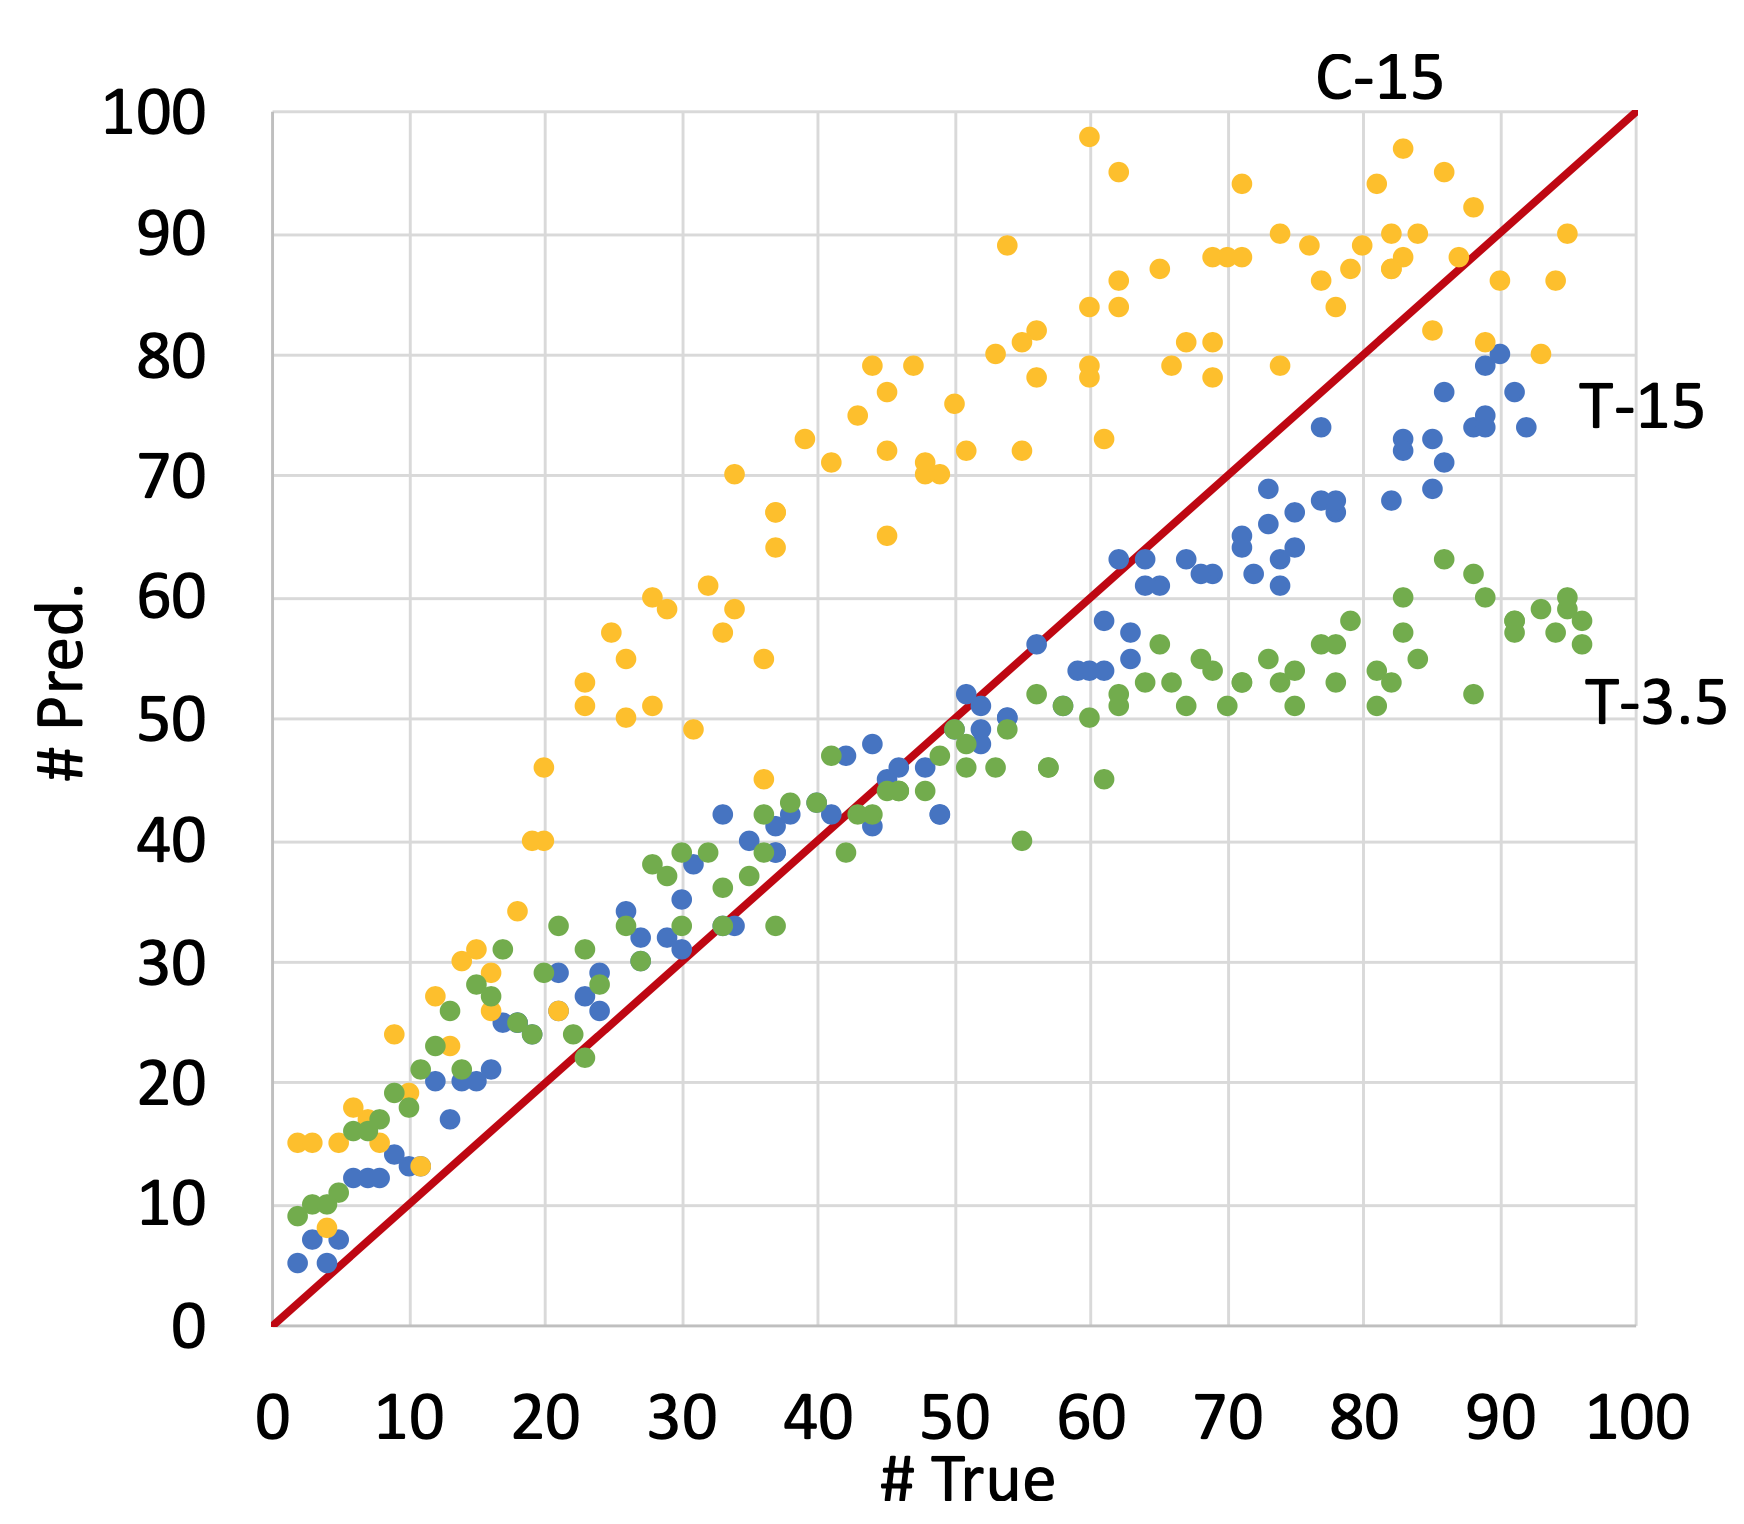
\includegraphics[width = 3in]{Counting/LaTeX/figures/nopropersubitization.png} & 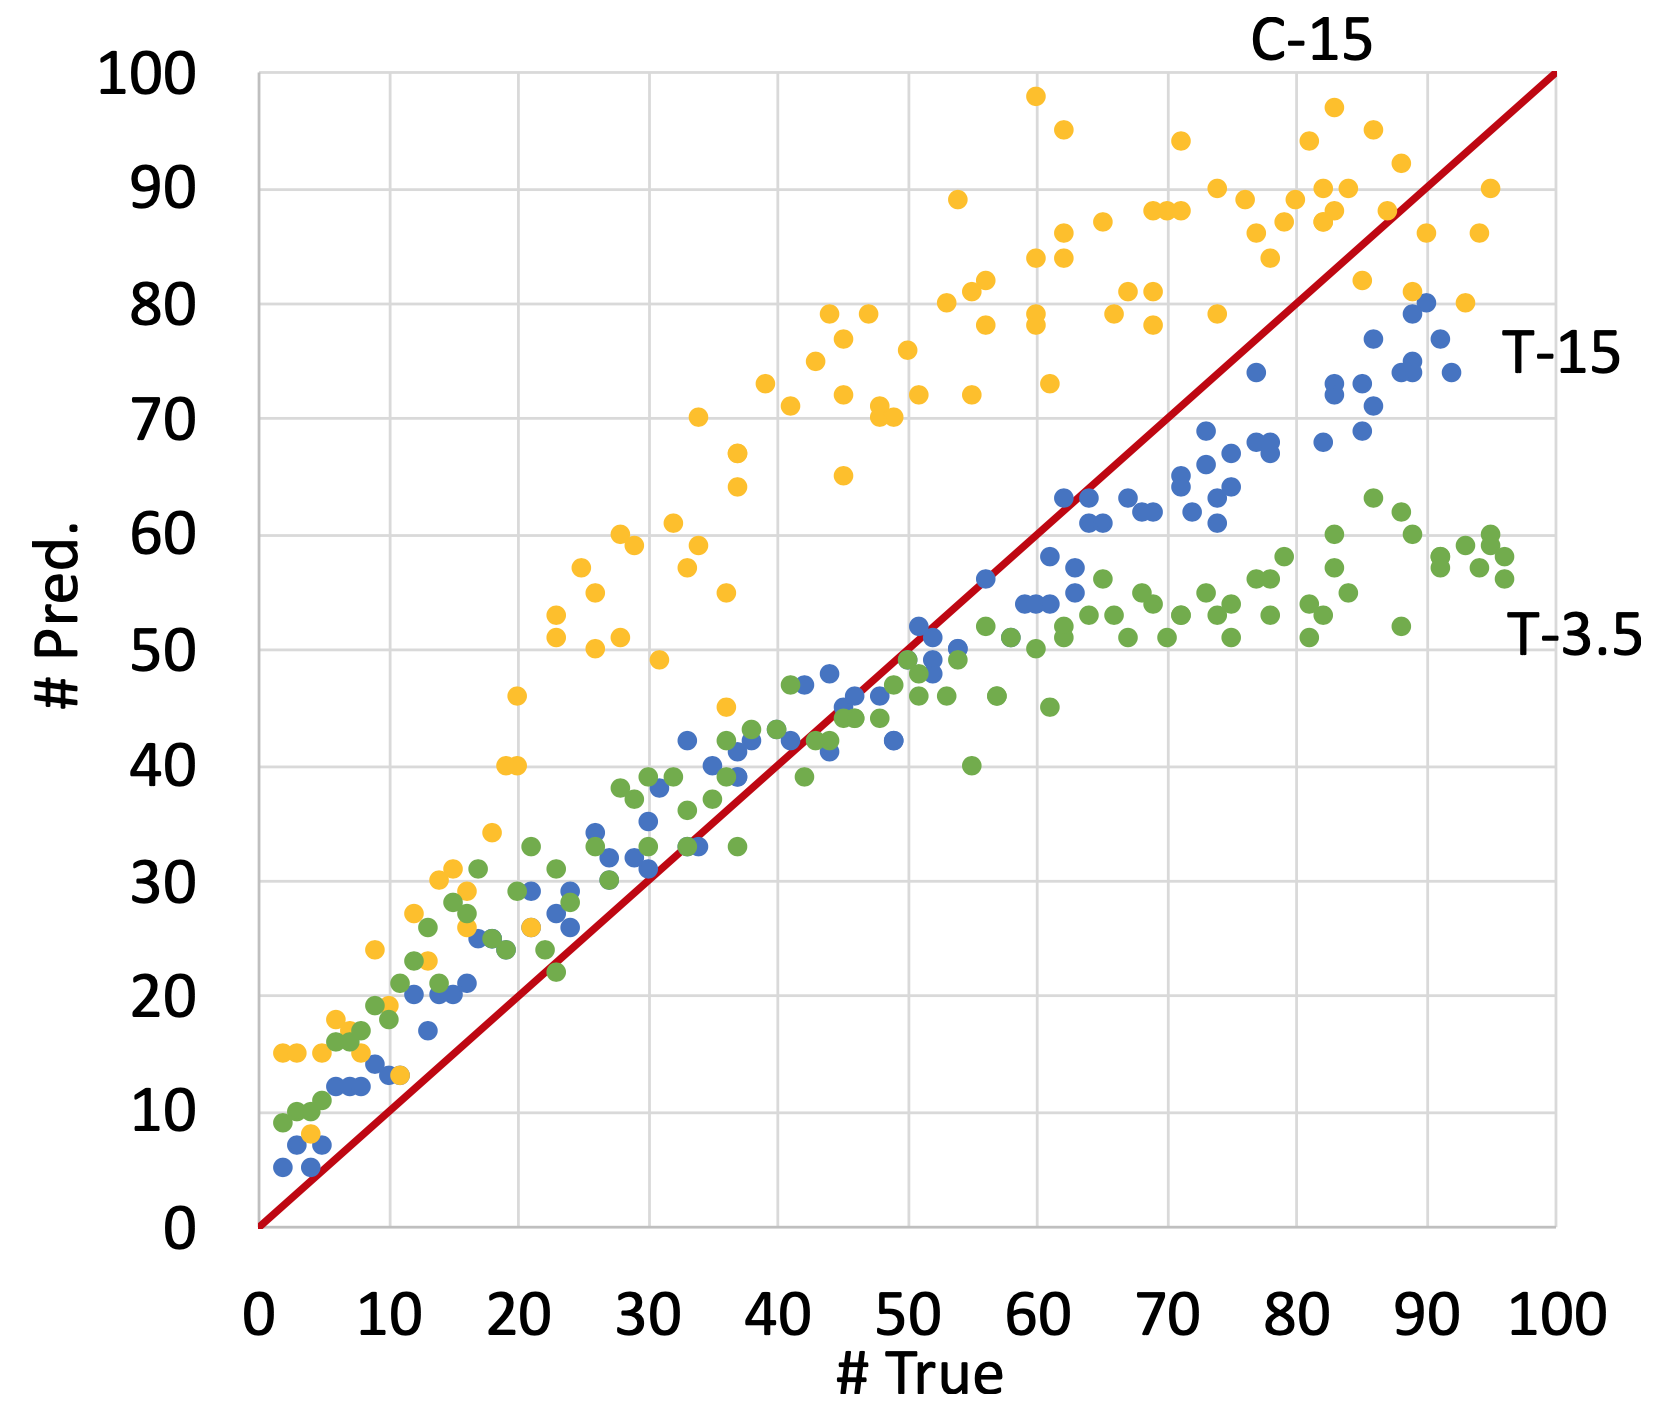
\includegraphics[width = 3in]{Counting/LaTeX/figures/successpartial.png} \\
            \textbf{a}                                                                     & \textbf{b}
        \end{tabular}
        \caption{\cite{guan2021understanding}[figures 4 and 7]'s performance graphs of the model
                 \cite{guan2021understanding} chose. Letters on graph grids refer to the first
                 letter of shapes triangle and circle, and the number after it is some measure of\
                 size.}
    \end{center}
    \label{nogeneralizationofshapes}
\end{figure}

We also refer to and discuss parts of this paper in section \ref{detectionasproofofrepresentation}.

\subsection{\textit{Deep Inside Convolutional Networks: Visualizing Image Classification Models and Saliency Maps} (Simonyan, Vedaldi, and Zisserman)}
One requirement of our methods specified in \ref{detectionasproofofrepresentation} is to be able
to understand the underlying representation the network ended up developing. Therefore, we present
\cite{simonyan2014deep}, which does not specifically explore counting, but will give us the tools
we need for our work.

\cite{simonyan2014deep} makes important contributions in two ways. The first is that they construct
a method by which a network can, in a sense, paint a picture that shows what the network thinks
a certain class looks like. They make the point that this method only describes the network, not
how the network comes to its conclusion on a per-sample basis. To do the latter task, they describe a method
of generating a saliency map, which we find very useful for our contributions.

In the general sense, a saliency map is an image where each pixel is given an intensity value
representing its contribution to the classification. In this paper, they work with the idea that
gradients w.r.t.\ an image is a direct saliency representation; backpropagation starts from the
desired class. The reasoning is intuitive: if the goal of a saliency map is to point out the most
salient parts of an image, then one can think of large gradients as essentially exactly what we need.
This is their method, but with a small modification: because each subpixel is assigned a gradient,
they merge the three as but there is only one value assigned to each pixel in the saliency map.
Merging consists of finding the channel with the greatest magnitude, and assign that magnitude to
the pixel for which we need to generate a value. They perform some sort of normalization as
the final values could be larger than 255 (or whatever limit the bit depth of the image implies).
Figure \ref{figure2simonyan} reproduces saliency maps that can be found in the paper.

\begin{figure}
    \begin{center}
        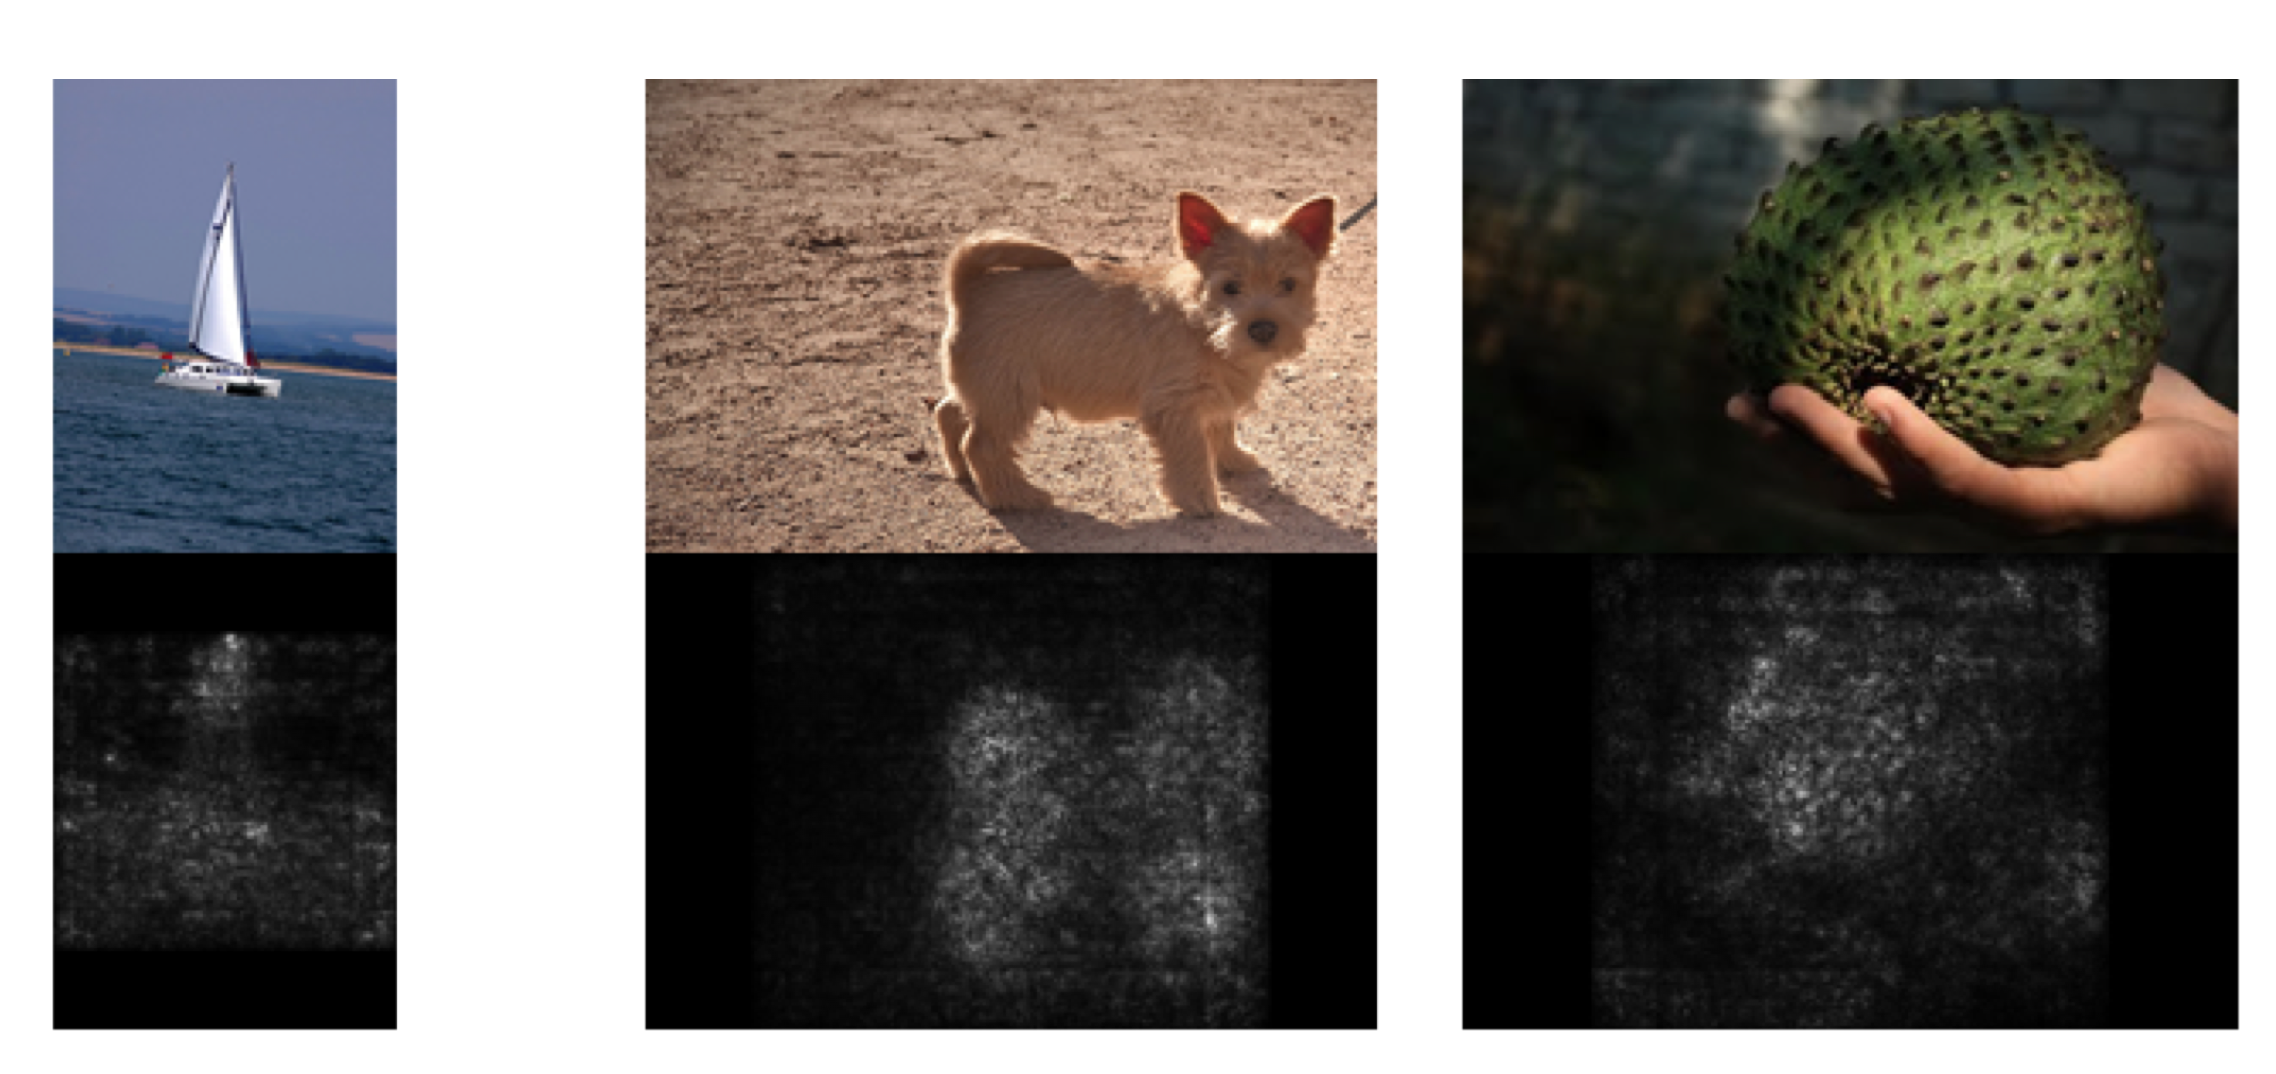
\includegraphics[width = \textwidth]{Counting/LaTeX/figures/simonyanfigure.png}
    \end{center}
    \caption{Some images and their respective saliencies they generated; from \cite{simonyan2014deep}[figure 2]}
    \label{figure2simonyan}
\end{figure}

Interestingly, they find that this saliency map can be used to determine which parts of the image
are foreground and background. This is due to the fact that the salient pixels are indications of
the foreground, and so they can be fed to an algorithm that performs the segmentation (they use
something in ~\cite{937505} to do the segmentation, but this author does not know the details of
that algorithm to elaborate how it works with the saliency map).

\section{The Network Whisperer}
\label{detectionasproofofrepresentation}
We tackle the same problem as is found in \cite{Zhang_2015_CVPR, guan2021understanding} of
subitization. However, there are a few differences between this implementation and each of those
implementations. In contrast to \cite{Zhang_2015_CVPR}, they work with a much wider definition of
subitization, in which the counter can count every kind of object; the domain is not restricted to
objects of the same type or roughly of the same type. We use a dataset that is extremely trivial
(uniform shapes in an image with a black backgroud) relative to their dataset. Though ambiguous
according to \cite{subitizingdefinition}, we believe that theirs is the correct interpretation,
especially from personal experience. Therefore, their problem is more difficult in this respect.
However, they stick with the common mindset of four objects being the maximum subitization
capability, and so compare their results to that limit (again, with a single category that pertains
to images with four or more objects). We do not believe this is a thorough test of the capabilities
of neural networks, and (though this fact was not a motivation for us) we take a stab at the neural
network learning to count an arbitrary number of objects. However, ``arbitrary'' does not mean
boundless as there can only be so many shapes within an image (a strong upper bound would be the
number of pixels in the image, but that is not a supremum). Both \cite{Zhang_2015_CVPR} and our work
attempt to detect objects using a classifier trained to count. However, our method performs the
localization as a byproduct of the second derivative of counting, which, although not exactly clear
due to time limits we had and ambiguity in the paper, differs from their methods; one of them uses
the output of the model as a guide for a separate counting method, for example.

% ^^^edit^^^: change "that" to "than"
With respect to \cite{guan2021understanding}, they make much stronger claims than this author feels
comfortable with. We aim to show that these networks can indeed subitize (up to a
object-dissimilarity limit), regardless of whether or not it is terribly accurate. Further, they
pose this problem as determining connected components, which allows them to make a claim that one
connecting pixel should be considered as merging two components into one. We think this is a dubious
argument, mostly because that for the example that they show~\cite{guan2021understanding}[figure
12], the vast majority of people would not likely be able to see the pixel-wide connection, and
therefore four separate components would have been the guess by most. Coincidentally, we also happen
to look at shapes, although we try to mix in different kinds and sizes of shapes into the same
image; they do try different sizes, but the sampling process is different (which we will use in our
implementation as a potential solution to poor saliency output).






The definition of our problem is as follows: given an image and a network, can we train the network
to successfully count shapes in a subitization fashion? The shapes were automatically generated with
random positioning; shape overlap detection was performed with the recommended\cite{viaforshapely}
Shapely\cite{shapely} package, and any overlap rejected that shape's location. Two possible shapes,
triangles and squares\footnote{This may be Professor David Crandall's idea} can be generated. Images
were drawn and saved with Pillow~\cite{imagesinpython}. Larger shapes resulted in proper learning;
we had no luck with smaller shapes. The network is a convolutional network, with no other layers
besides activation functions and a linear layer at the end to output a single
ReLU\cite{pmlr-v15-glorot11a}\footnote{This reference is commonly pointed to as the source of
ReLU}-filtered number. This is done because the network~\cite{szegedy2014going} they use in
\cite{10.1007/978-3-319-46487-9_48} does as well (except for the output layer). The loss function is
mean squared error, with the ground truth being the raw number of each kind of shape (this is in
contrast to \cite{Zhang_2015_CVPR}, which had separate classes that represented different counts).
Because the images are automatically generated, we are able to use extremely large datasets, which
may not be a reasonable expectation when training on non-artificial data. For now, we stick with
shapes as it is a simplified problem for which a proof-of-concept could lead to further research
into whether the concept can be applied in the real world (not just from a subitization standpoint,
but also from a detection one as well). We used Chainer~\cite{tokui2019chainer} to implement our
research in this section, as well as CuPy~\cite{cupy_learningsys2017}, NumPy~\cite{2020NumPy-Array},
and Python 3~\cite{language}. There was previous code that addressed this topic based on
PyTorch~\cite{NEURIPS2019_9015}; we did use it to some extent, but it was rewritten to use Chainer
later on. This code may have used Nesterov momentum instead.

\subsection{Detecting Shapes}
\label{detectingshapes}

To perform the detection step, a trained network\footnote{trained with small batch sizes as we found
this useful for some reason; it could be that small batch sizes increase variance, which results in
kind of a simulated annealing-like behavior} and an image are used to generate a saliency map via
the method described in \cite{simonyan2014deep}. However, instead of backpropagating from the
correct class's output (there is no concept of ``class'' in our network), we backpropagate from the
addition of all the outputs (which ideally would give us the total number of shapes), one output
squares and one for triangles. This addition occurs (most likely; thank the author's short memory)
because the aim is to detect \textit{all} shapes within the image, not just one type; however, it
would be good to see if saliency for a single shape type could be used (depending on the success of
the original method, of course).

The detection step comes in by exploiting the (yet unproven) property that the gradient of one pixel
depends on the value of another. Ideally, if the derivative of the saliency of the pixel w.r.t.
another pixel changes, then that implies that the changing value of the latter pixel (for this
example, it decreases to become more like the background) causes the former to take on more of a
representational burden in order to keep the object count up. However, it is possible that every
pixel in the image can change the second derivative of the target pixel. To see why, let's look at
the first derivative w.r.t. the image ($f$ is the sum over the estimated shape count, $x_i$ is
subpixel $i$ of image $x$, and $a_k$ is the output of layer $k$ for image $x$):
\[
    \frac{\partial f}{\partial x_i} = \frac{\partial f}{\partial a_k} \frac{\partial a_k}{\partial x_i}
\]
If we take the partial derivative of $\frac{\partial f}{\partial x_i}$ w.r.t. subpixel $j$, we see
that the product rule gives us non-zero values for some or all parts of the domain following what is
shown in section \ref{gradientmagnitudereduction}; the difference here is that we don't use a
non-linear loss function, so at least one activation function for this network \textit{must} be
non-linear (even if the function is piecewise, as described in \ref{gradientmagnitudereduction}) for
this to be true. We do not go over why not all layers have to have a non-zero second derivative in
that section (although work on the topic of \ref{gradientmagnitudereduction} likely preceded, and
therefore was the foundation of, this the idea of the type of activation causing second-order
issues), so we will do that here. Here is the analytical derivation of the second derivative:
\begin{multline*}
    \frac{\partial}{\partial x_j}     \frac{\partial a_4}{\partial a_3} \frac{\partial a_3}{\partial a_2} \frac{\partial a_2}{\partial a_1} \frac{\partial a_1}{\partial x_i} = \\[10pt]
    \frac{\partial f_3}{\partial x_i}  \left( \frac{\partial}{\partial x_j} \frac{\partial a_4}{\partial a_3} \right)       +       \frac{\partial a_4}{\partial a_3} \left( \frac{\partial}{\partial x_j} \frac{\partial f_3}{\partial x_i} \right)\\[10pt] 
    = \frac{\partial f_3}{\partial x_i}  \left( \frac{\partial}{\partial x_j} \frac{\partial a_4}{\partial a_3} \right)       +       \frac{\partial a_4}{\partial a_3}         \left[     
                \frac{\partial f_2}{\partial x_i}  \left( \frac{\partial}{\partial x_j} \frac{\partial a_3}{\partial a_2} \right)       +       \frac{\partial a_3}{\partial a_2} \left( \frac{\partial}{\partial x_j} \frac{\partial f_2}{\partial x_i} \right)
      \right]\\[10pt]
    = \frac{\partial f_3}{\partial x_i}  \left( \frac{\partial}{\partial x_j} \frac{\partial a_4}{\partial a_3} \right)       +       \frac{\partial a_4}{\partial a_3}         \left[     
                \frac{\partial f_2}{\partial x_i}  \left( \frac{\partial}{\partial x_j} \frac{\partial a_3}{\partial a_2} \right)       +       \frac{\partial a_3}{\partial a_2}          \left[
                        \frac{\partial f_1}{\partial x_i}  \left( \frac{\partial}{\partial x_j} \frac{\partial a_2}{\partial a_1} \right)       +       \frac{\partial a_2}{\partial a_1} \left( \frac{\partial}{\partial x_j} \frac{\partial f_1}{\partial x_i} \right)
                \right]
      \right]\\[10pt]
    = \frac{\partial f_3}{\partial x_i}  \left( \frac{\partial}{\partial x_j} \frac{\partial a_4}{\partial a_3} \right)       +       \frac{\partial a_4}{\partial a_3}         \left[     
                \frac{\partial f_2}{\partial x_i}  \left( \frac{\partial}{\partial x_j} \frac{\partial a_3}{\partial a_2} \right)       +       \frac{\partial a_3}{\partial a_2}          \left[
                        \frac{\partial f_1}{\partial x_i}  \left( \frac{\partial}{\partial x_j} \frac{\partial a_2}{\partial a_1} \right)       +       \frac{\partial a_2}{\partial a_1} \left( \frac{\partial}{\partial x_j} \frac{\partial a_1}{\partial x_i} \right)
                \right] 
      \right]
\end{multline*}
We can simplify this rather complex series of additions, and this looks like
\begin{multline*}
     \frac{\partial f_3}{\partial x_i}  \left( \frac{\partial}{\partial x_j} \frac{\partial a_4}{\partial a_3} \right)       +       \frac{\partial a_4}{\partial a_3}         \left[     
                \frac{\partial f_2}{\partial x_i}  \left( \frac{\partial}{\partial x_j} \frac{\partial a_3}{\partial a_2} \right)       +       \frac{\partial a_3}{\partial a_2}          \left[
                        \frac{\partial f_1}{\partial x_i}  \left( \frac{\partial}{\partial x_j} \frac{\partial a_2}{\partial a_1} \right)       +       \frac{\partial a_2}{\partial a_1} \left( \frac{\partial}{\partial x_j} \frac{\partial a_1}{\partial x_i} \right)
                \right] 
      \right]\\[10pt]
     = \frac{\partial f_3}{\partial x_i}  \left( \frac{\partial}{\partial x_j} \frac{\partial a_4}{\partial a_3} \right)       +       \frac{\partial a_4}{\partial a_3}         \left[     
                \frac{\partial f_2}{\partial x_i}  \left( \frac{\partial}{\partial x_j} \frac{\partial a_3}{\partial a_2} \right)       +
                         \frac{\partial a_3}{\partial a_2} \frac{\partial f_1}{\partial x_i}  \left( \frac{\partial}{\partial x_j} \frac{\partial a_2}{\partial a_1} \right)       +        \frac{\partial a_3}{\partial a_2} \frac{\partial a_2}{\partial a_1} \left( \frac{\partial}{\partial x_j} \frac{\partial a_1}{\partial x_i} \right)
       \right]\\[10pt]
     = \frac{\partial f_3}{\partial x_i}  \left( \frac{\partial}{\partial x_j} \frac{\partial a_4}{\partial a_3} \right)       +    
                \frac{\partial a_4}{\partial a_3} \frac{\partial f_2}{\partial x_i}  \left( \frac{\partial}{\partial x_j} \frac{\partial a_3}{\partial a_2} \right)       +
                         \frac{\partial a_4}{\partial a_3} \frac{\partial a_3}{\partial a_2} \frac{\partial f_1}{\partial x_i}  \left( \frac{\partial}{\partial x_j} \frac{\partial a_2}{\partial a_1} \right)       +
                                \frac{\partial a_4}{\partial a_3} \frac{\partial a_3}{\partial a_2} \frac{\partial a_2}{\partial a_1} \left( \frac{\partial}{\partial x_j} \frac{\partial a_1}{\partial x_i} \right)
\end{multline*}
We can expand this process to any number of layers. However, if each activation function has a
second derivative of $0$, the whole equation collapses to $0$; we discuss why this is relevant and a
problem shortly. If the last activation function's gradient has a gradient that is non-zero, then we
cannot guarantee the network's complete second derivative will end up being zero at some subpixel
$x_j$. This is essentially the same point that \ref{gradientmagnitudereduction} makes (and it may
have been based on it too). This conclusion requires that the derivatives of the derivatives of an
activation with respect to another evaluate (for example, $\left( \frac{\partial}{\partial x_j}
\frac{\partial a_4}{\partial a_3} \right)$) to zero. This happens to be the case because the second
derivative between two layers is zero, and the left-over derivative of the incoming set of
activations w.r.t. $x_j$ due to the chain rule application are nullified because it is multiplied by
the aforementioned second derivative. So, avoiding zero-valued second derivatives is necessary (one
non-zero second derivative will possibly result in a non-zero, end-to-end second derivative because
every addition in the above equation could give us something non-zero)\footnote{Stefan Lee confirmed
my math (at least for ReLU) as he also believed that $\frac{\partial^2 f}{\partial x_i}$ is required
to be non-zero}.

\subsection{Algorithm}
\label{algorithm}

Now that we have established the basic concepts and requirements for our localization procedure, we
can outline ways in which detection may happen. A way that we attempted (but were never able to
fully iron-out) and inspired by the thresholding used in \cite{reeves}[3:58] is that we take the
highest saliency~\cite{simonyan2014deep} value (which corresponds to a certain pixel $i$), and then
calculate the second derivative of that value w.r.t.\ each pixel within the image (forming a
saliency map in the same way that \cite{simonyan2014deep} does, but using the second derivative ---
this was done to ensure that second derivative values do not become negative when formulated as
saliency due to the absolute value used in \cite{simonyan2014deep}, and also to merge the three
channels of derivatives that would result under normal partial derivative calculation of the first
saliency map; this is why \cite{simonyan2014deep} takes these steps). We choose to backpropagate
from the most salient pixel as, intuitively, that is the pixel most likely to be on a shape. We then
threshold the second-derivative using some kind of intelligently chosen value, giving us a set of
pixels that hopefully are related enough to the original pixel. Using this set, it is possible to
draw a bounding-box around them, giving us detection. After this, we remove these pixels (including
the one from which we backpropagated) from the set of unassigned pixels. We do this for each $i$
(where $i$ is from the remaining pixels) until we no longer have no more shapes to find (based on
the count output by the network).

% Other papers^^^^^^ that do qualitative analysis look into results without it being in a dedicated
% results section, so I decided that it is OK for me to do that here (don't remember if I used those
% previous works for this reason before I started writing this, or as justification for keeping it
% the way I have it while I was writing this).
Unfortunately, we did not find this method reliable. For starters, the second derivatives only
covered, at most, about half of the shape, which would leave us with an incomplete bounding box.
This could be due to a poorly-chosen threshold value, but we did not have enough time to try other
values. However, we also noticed that a lot of the selected second-derivative pixels were between
two shapes, which obviously would cause poor localization. This is actually not that surprising;
remember, the first derivative was the derivative for the predicted count. If a pixel in-between is
chosen as $i$, then it likely influence the part of the total count that corresponds to the two
shapes; as a result, it would not be surprising that pixels local to $i$ would determine $i$'s first
derivative (say, if a new shape started to form using those children pixels). It is important to
note that the case before this could be because these shapes were further away than others. However,
as one can see in figure \ref{shapecorrelation}, the spatial breadth of the selected pixels is not
nearly the same, so we may be able to make the claim that we did anyway. Another issue is that, as
the loop continued, fewer shape-like structures formed by the second derivative were selected; many
of the points were extremely local. A more intelligent pixel selection method would likely improve
this method substantially. Regardless, we definitely see promising results (see figure
\ref{shapecorrelation}) that make it clear (barring any missed strange scenarios that allow these
images) that the network is probably learning some form of representation, especially because figure
\ref{inputs} show that the most saliency is being placed on the edges and the corners, what are
likely the only features that these shapes have. The original image and its saliency can be seen in
figure \ref{inputs}. Note that all experimental saliency pictures, including those for the
saliencies of the saliency, have slight tweaks to them: we have taken the 10th root of each saliency
output pixel so that the extrema are closer together, thus improving image readability, and they
were normalized for image output (this applies only to saliency maps, not the thresholded images).
Further, Pillow was used to transform this output to image files. This also applies to the saliency
maps generated for each saliency pixel. This is inspired by plots that use the log scale on the
y-axis.

\begin{figure}[th]
    \begin{center}
        \begin{tabular}{c c}
            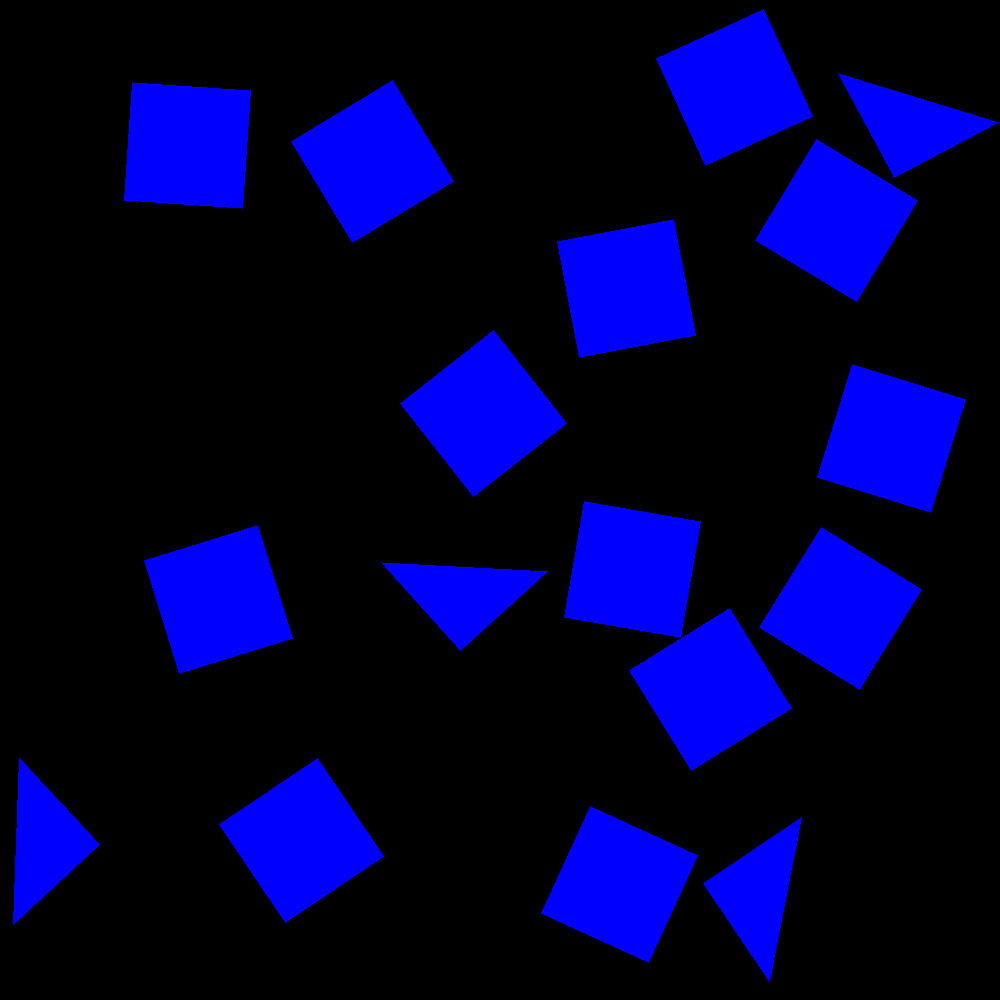
\includegraphics[width=2in, height=2in]{Counting/LaTeX/figures/putasideall/limitscaleresamplingoptionnetworkputaside/image1/touse/001.png} & 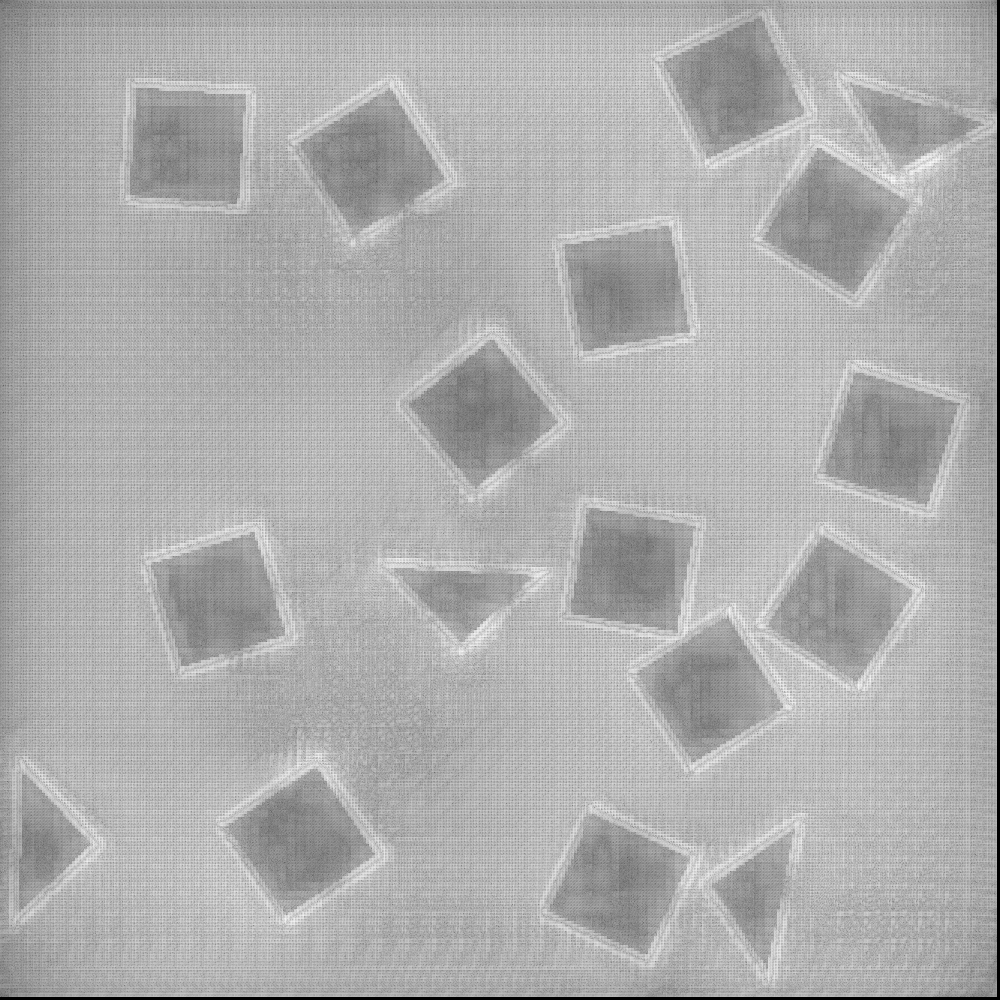
\includegraphics[width=2in, height=2in]{Counting/LaTeX/figures/putasideall/limitscaleresamplingoptionnetworkputaside/image1/touse/saliency.png} \\
            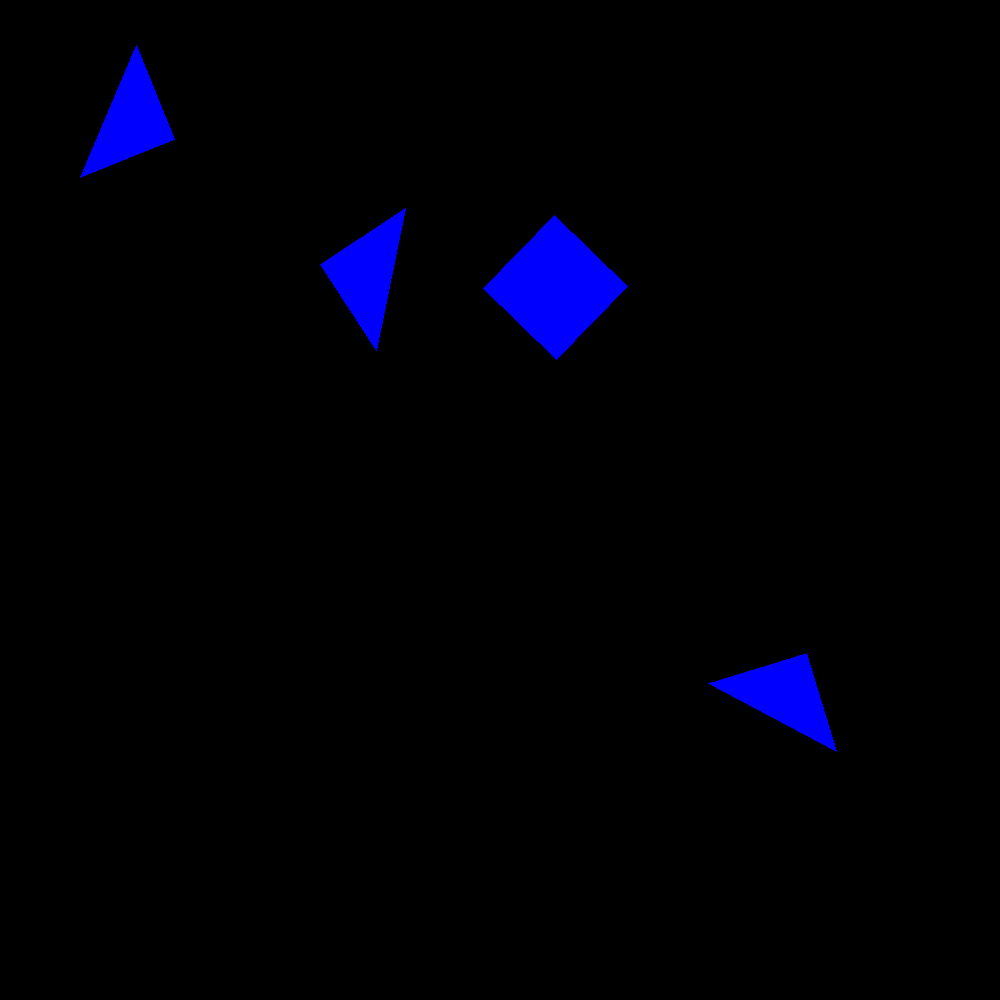
\includegraphics[width=2in, height=2in]{Counting/LaTeX/figures/putasideall/limitscaleresamplingoptionnetworkputaside/image2/touse/007.png} & 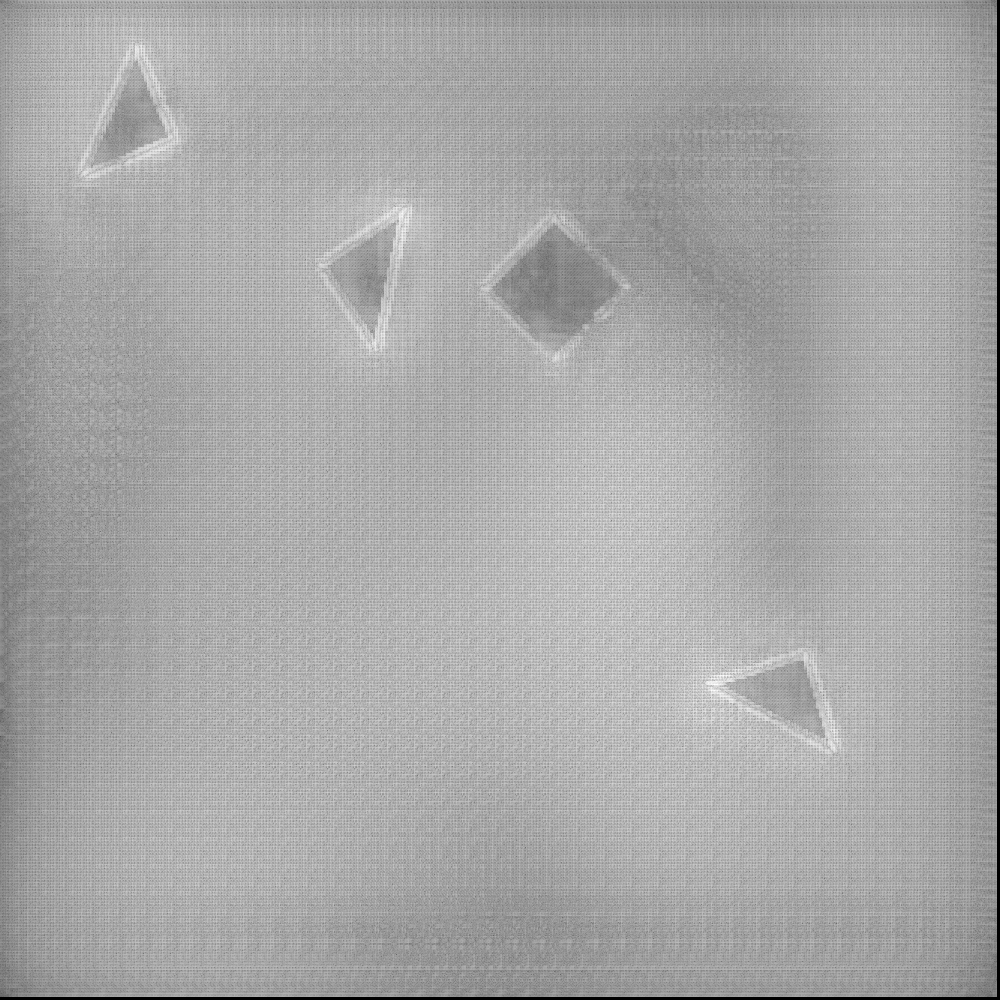
\includegraphics[width=2in, height=2in]{Counting/LaTeX/figures/putasideall/limitscaleresamplingoptionnetworkputaside/image2/touse/saliency.png}
        \end{tabular}
    \end{center}
    \caption{The first image is the image that the network sees, while the second image is the
             saliency for that image}
    \label{inputs}
\end{figure}

\begin{figure}[t]
    \begin{center}
        \begin{tabular}{c c c}
            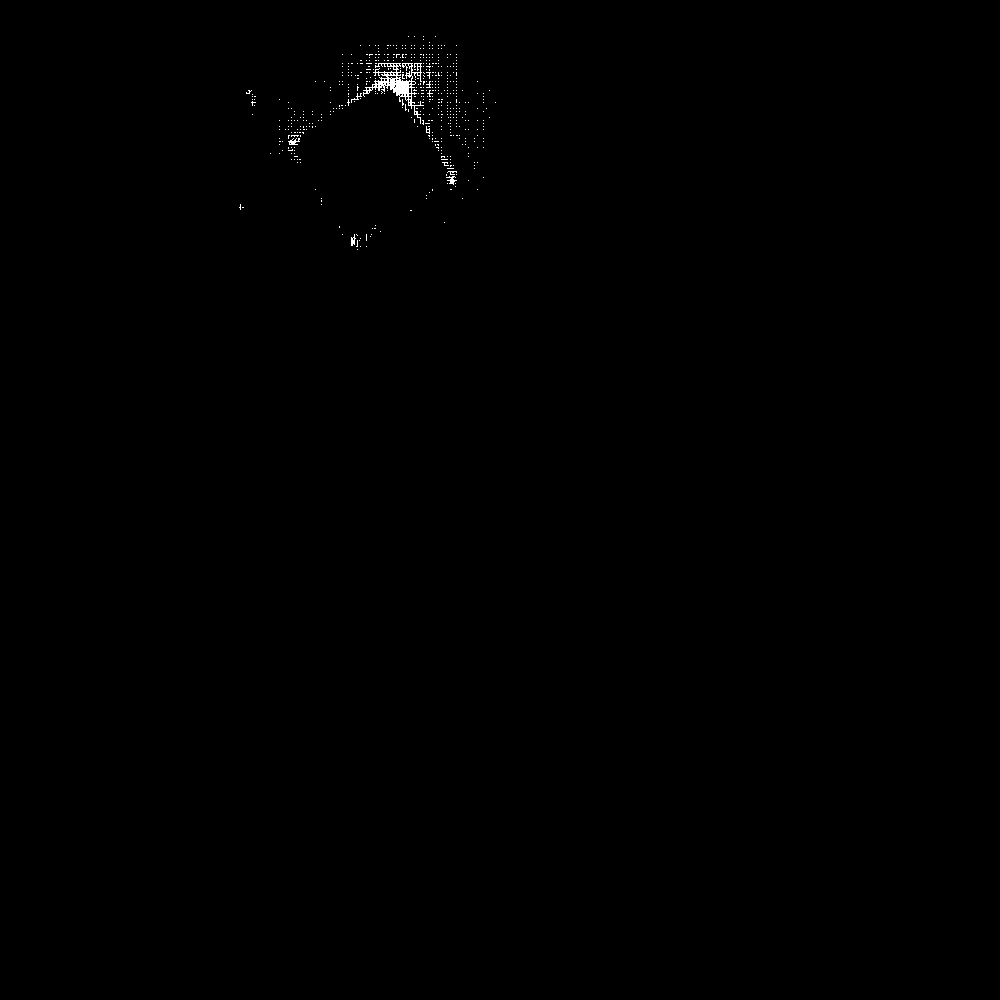
\includegraphics[width=1.5in, height=1.5in]{Counting/LaTeX/figures/putasideall/limitscaleresamplingoptionnetworkputaside/image1/touse/8.png}          & 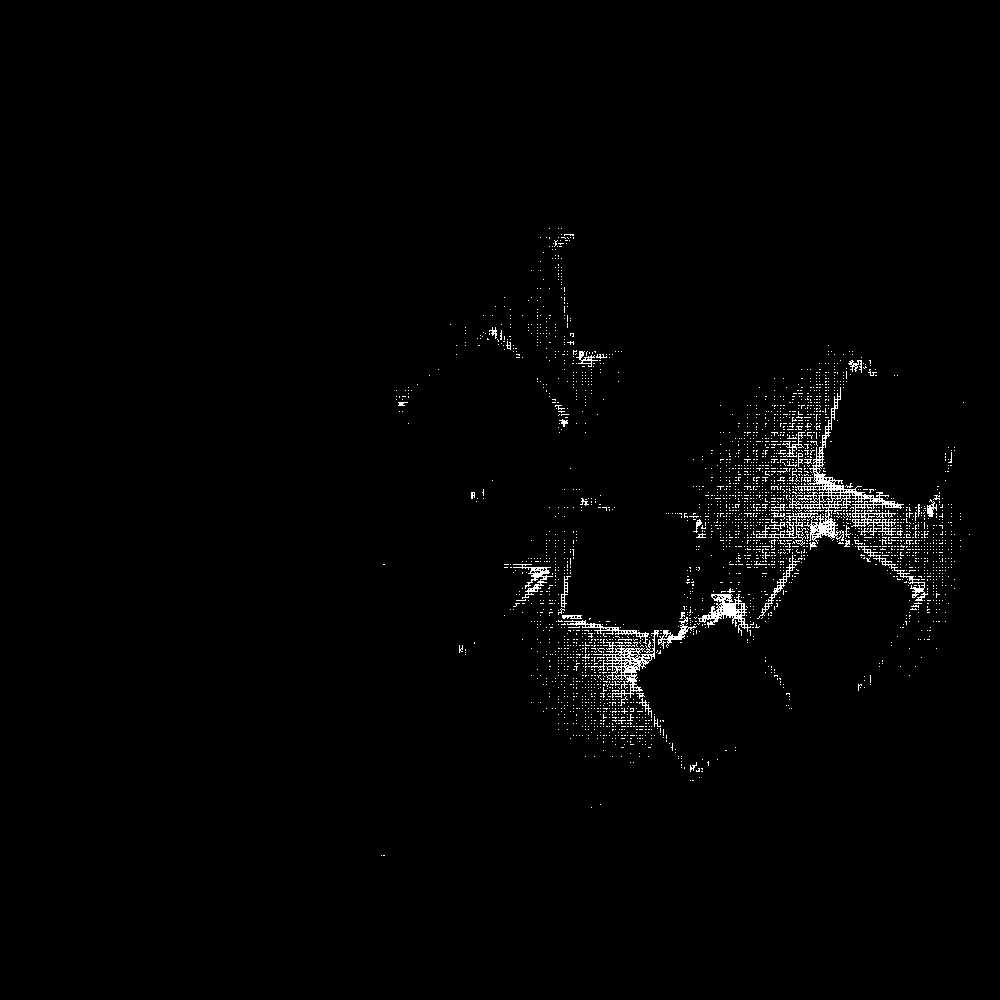
\includegraphics[width=1.5in, height=1.5in]{Counting/LaTeX/figures/putasideall/limitscaleresamplingoptionnetworkputaside/image1/touse/2.png}          & 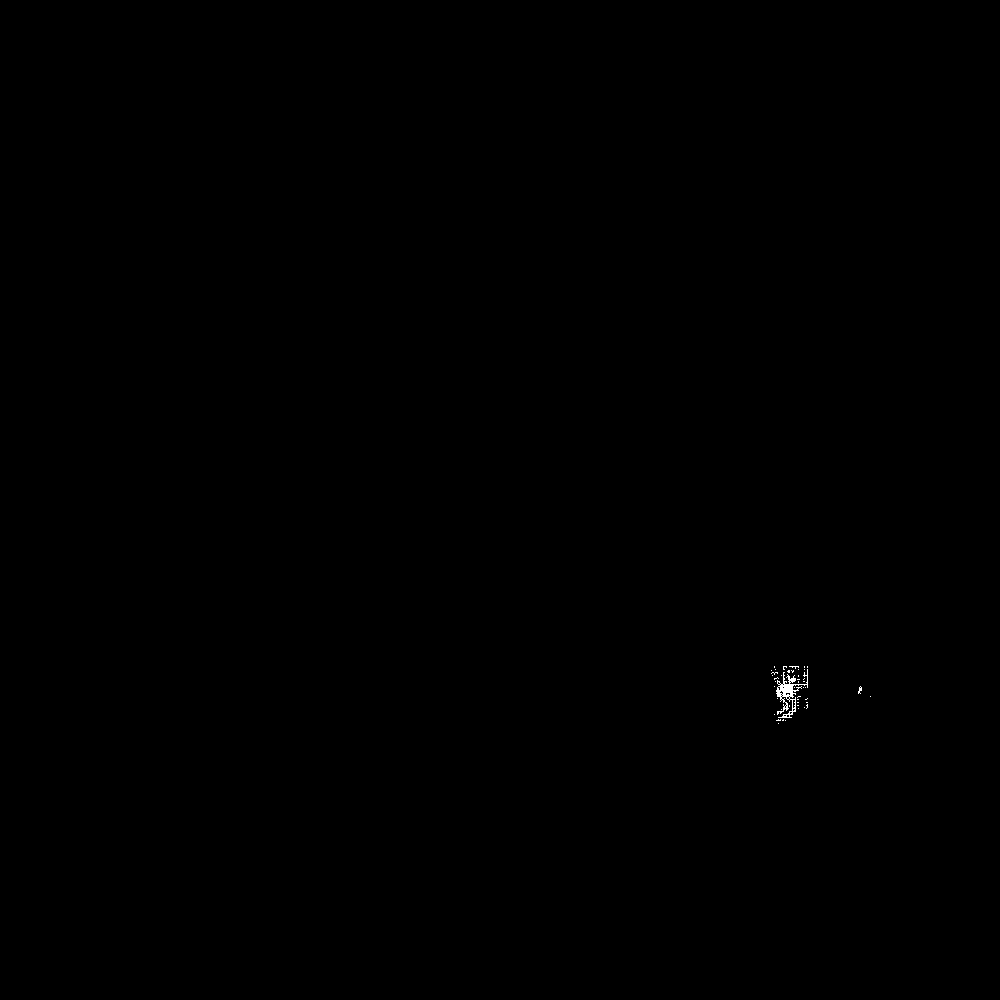
\includegraphics[width=1.5in, height=1.5in]{Counting/LaTeX/figures/putasideall/limitscaleresamplingoptionnetworkputaside/image1/touse/17.png}          \\
            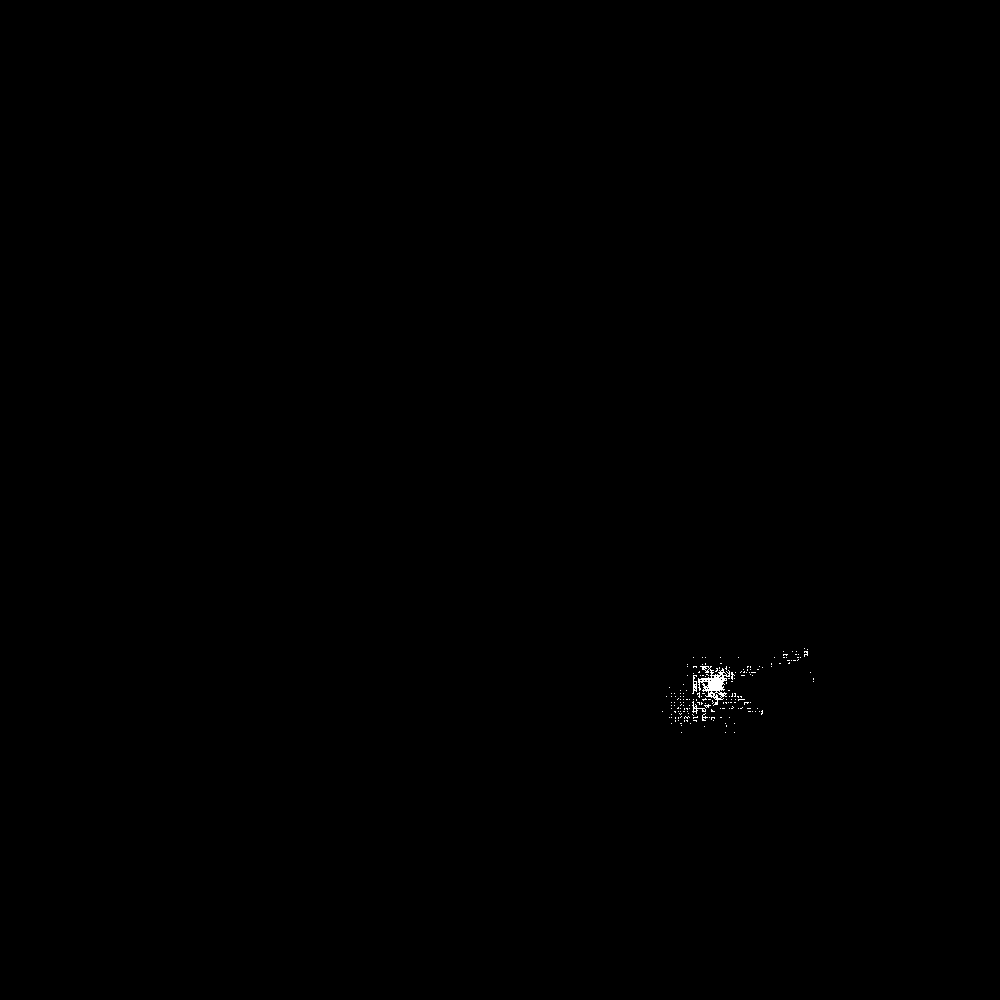
\includegraphics[width=1.5in, height=1.5in]{Counting/LaTeX/figures/putasideall/limitscaleresamplingoptionnetworkputaside/image2/touse/1.png}          & 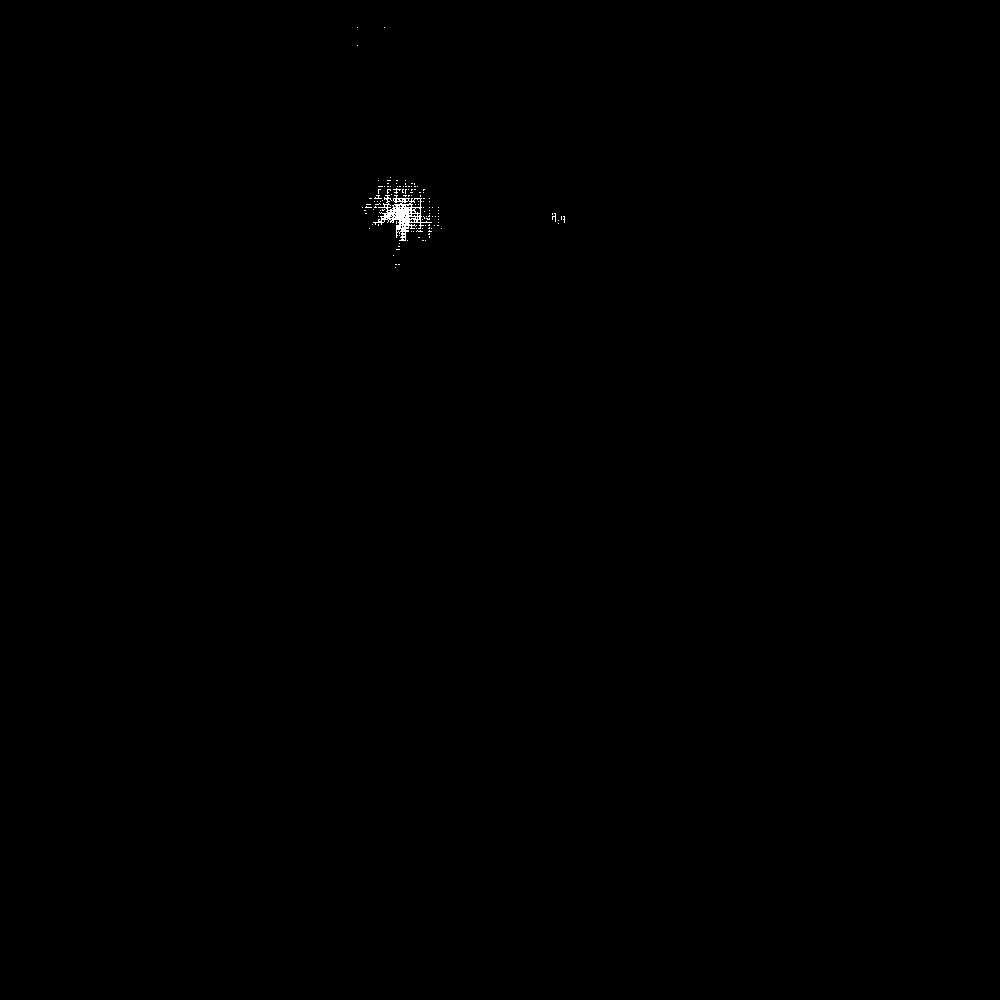
\includegraphics[width=1.5in, height=1.5in]{Counting/LaTeX/figures/putasideall/limitscaleresamplingoptionnetworkputaside/image2/touse/2.png}          & 
\includegraphics[width=1.5in, height=1.5in]{Counting/LaTeX/figures/putasideall/limitscaleresamplingoptionnetworkputaside/image2/touse/3.png}           \\
            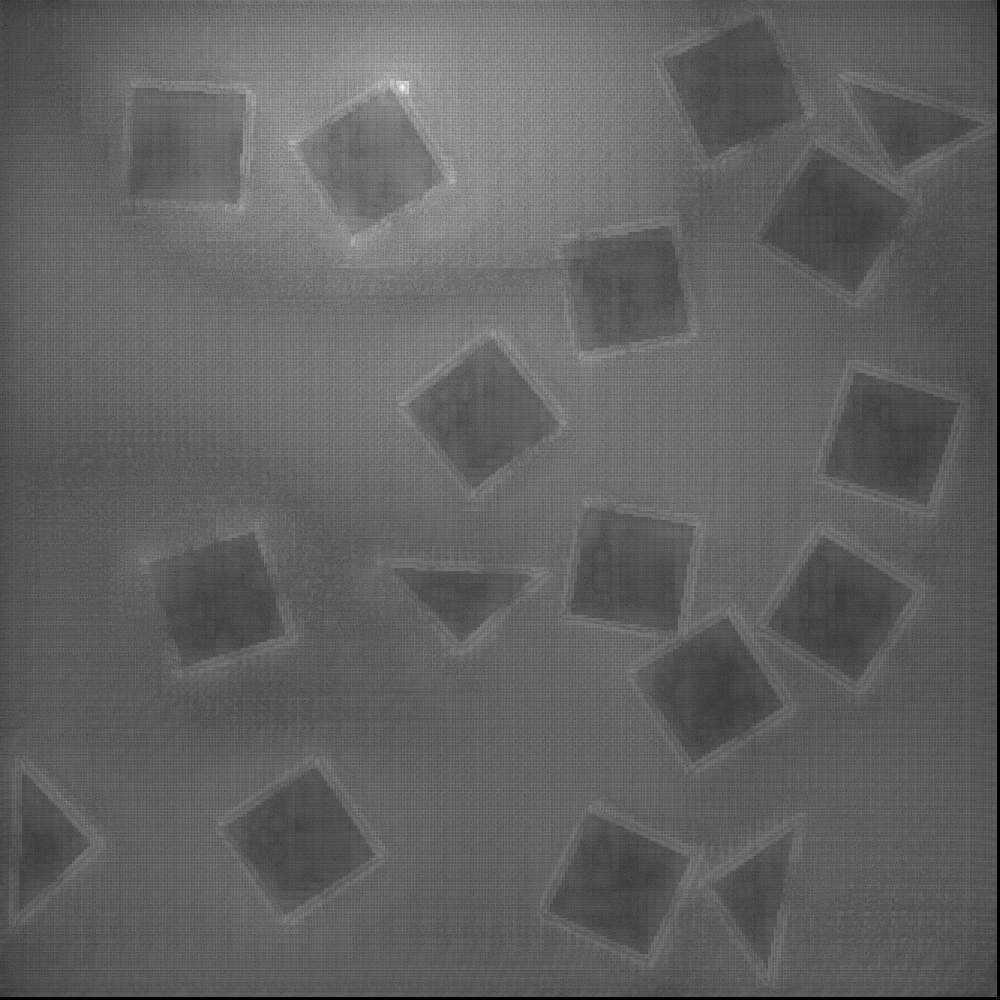
\includegraphics[width=1.5in, height=1.5in]{Counting/LaTeX/figures/putasideall/limitscaleresamplingoptionnetworkputaside/image1/touse/8-saliency.png} & 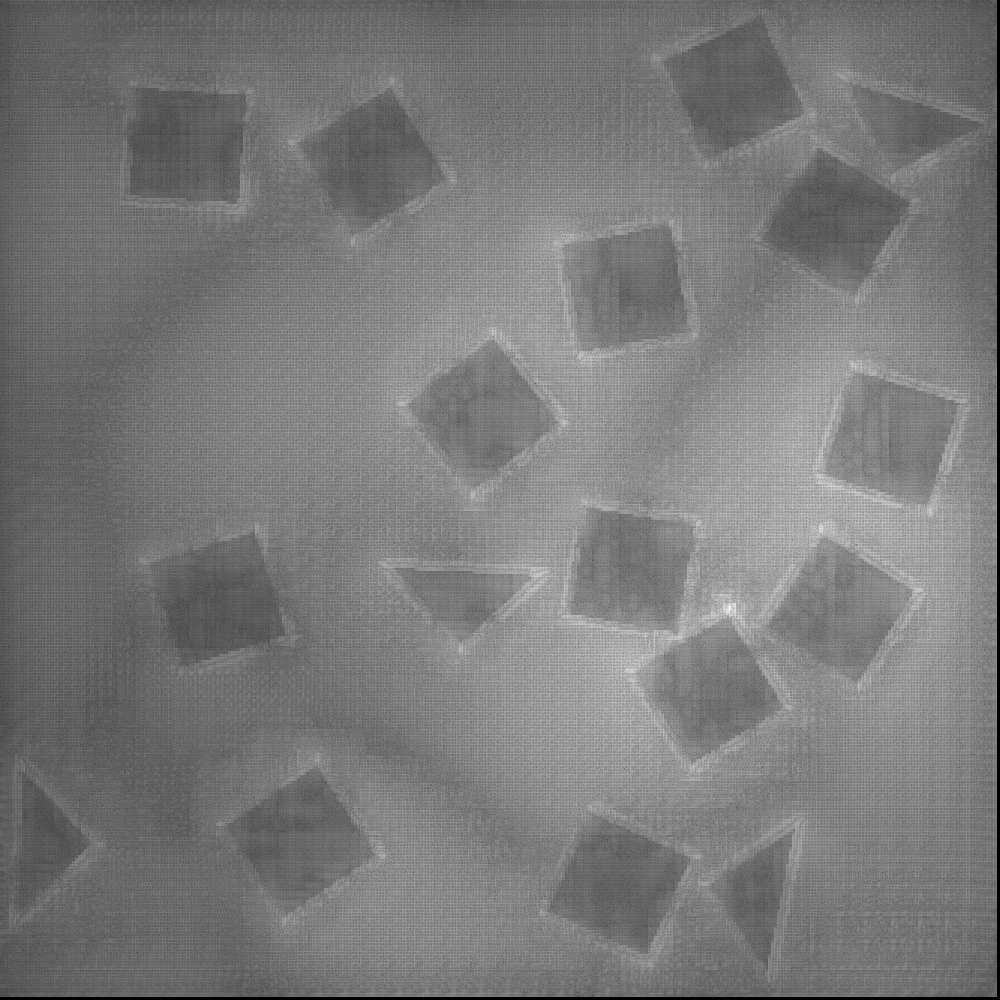
\includegraphics[width=1.5in, height=1.5in]{Counting/LaTeX/figures/putasideall/limitscaleresamplingoptionnetworkputaside/image1/touse/2-saliency.png} & 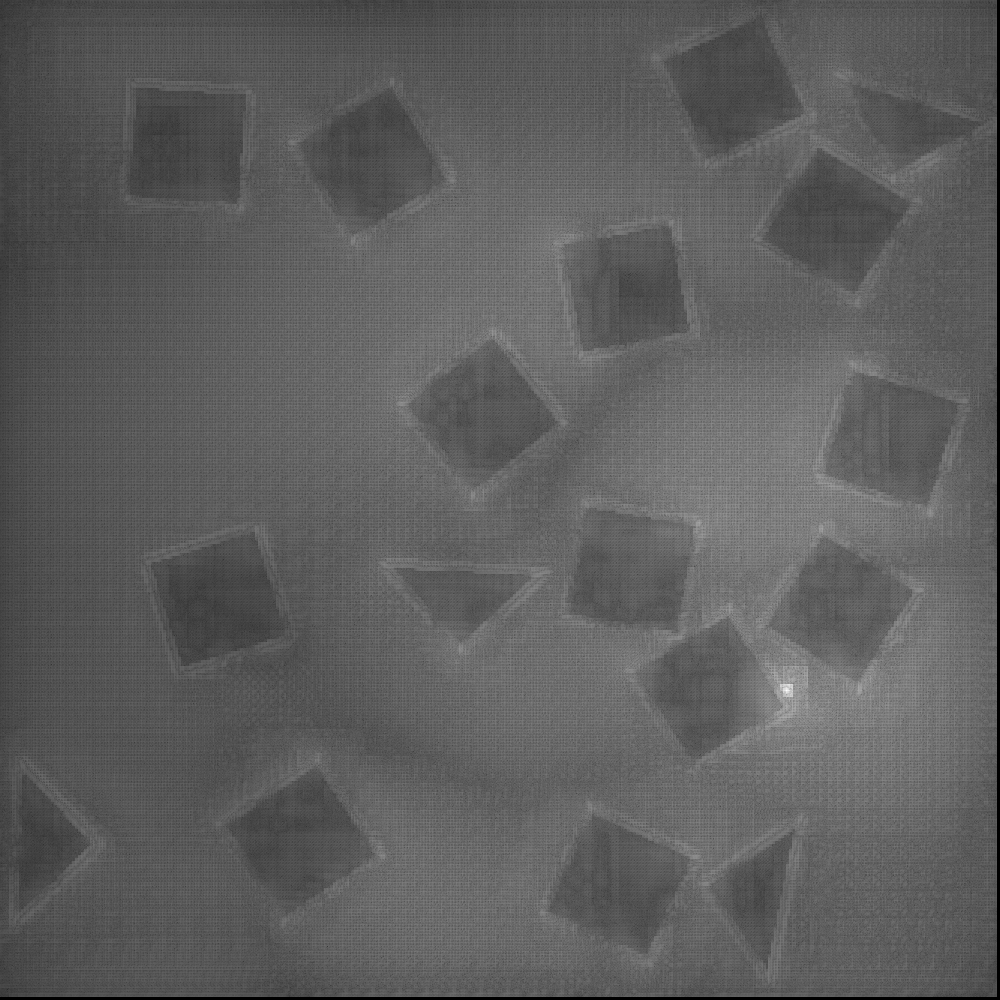
\includegraphics[width=1.5in, height=1.5in]{Counting/LaTeX/figures/putasideall/limitscaleresamplingoptionnetworkputaside/image1/touse/17-saliency.png} \\
            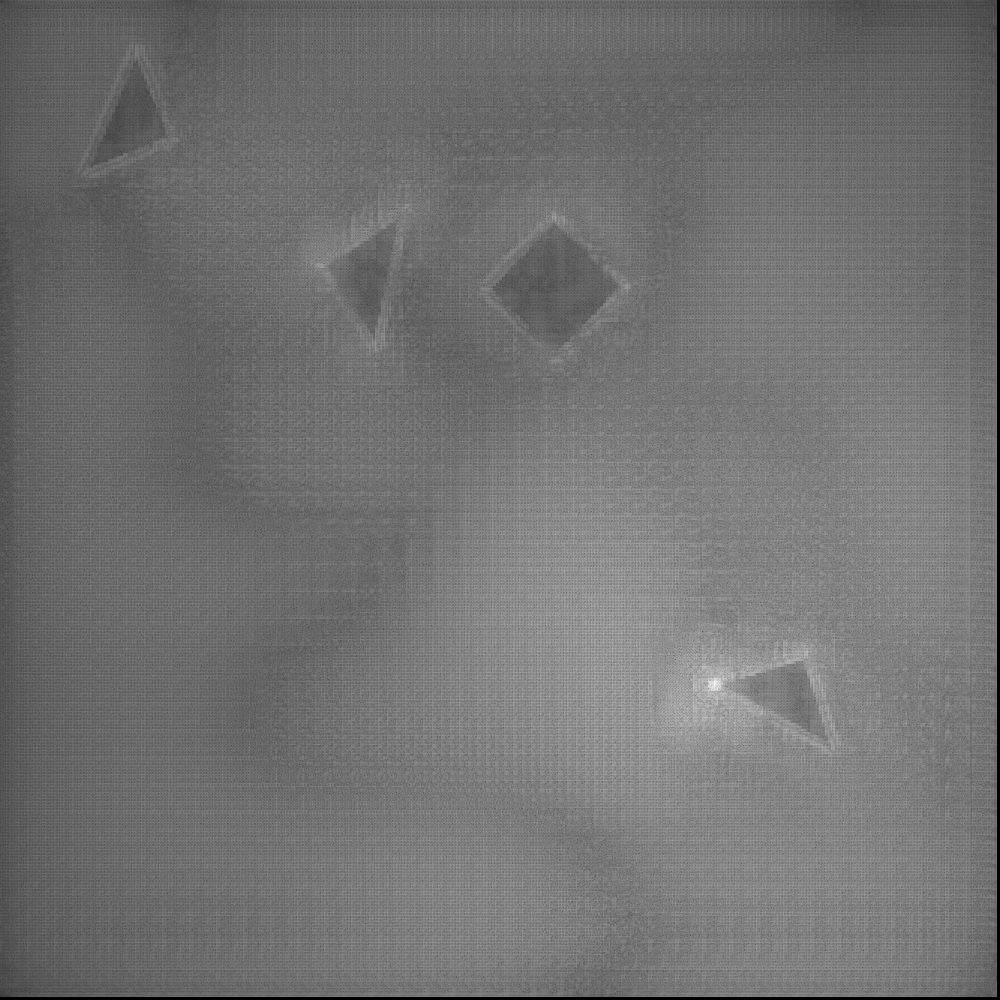
\includegraphics[width=1.5in, height=1.5in]{Counting/LaTeX/figures/putasideall/limitscaleresamplingoptionnetworkputaside/image2/touse/1-saliency.png} & 
\includegraphics[width=1.5in, height=1.5in]{Counting/LaTeX/figures/putasideall/limitscaleresamplingoptionnetworkputaside/image2/touse/2-saliency.png} & 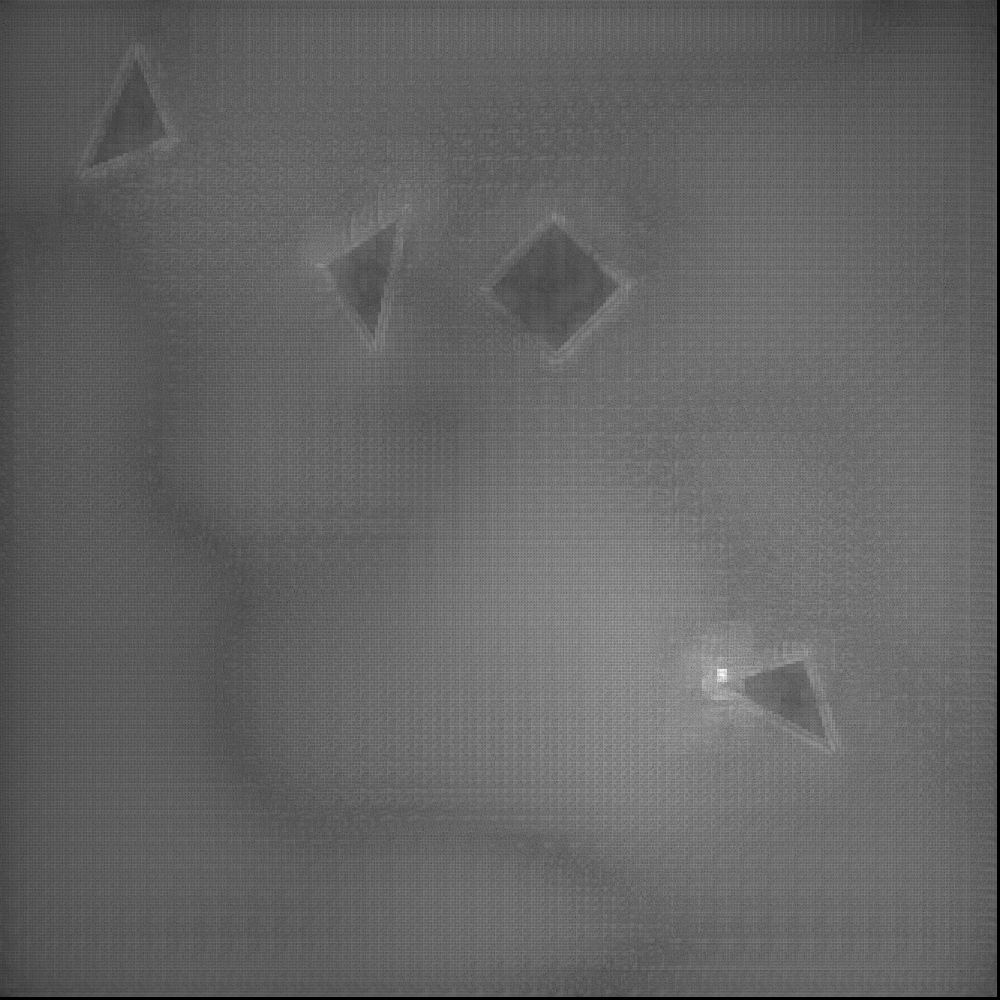
\includegraphics[width=1.5in, height=1.5in]{Counting/LaTeX/figures/putasideall/limitscaleresamplingoptionnetworkputaside/image2/touse/3-saliency.png}
        \end{tabular}
    \end{center}
    \caption{Each of the first two row represents a different image. The first images for these
             clearly shows the partial outline of a shape, while the second depicts the situation of
             a pixel being associated with multiple shapes. The third is the case where saliency
             selection derails and the area selected is not, or partially not, meaningful. Their
             full maps before thresholding are in the third and fourth rows.}
    \label{shapecorrelation}
\end{figure}



\subsection{Tweaks}



Initially, our ReLU-activated network was trained on images of shapes that did not vary in size.
Prediction was extremely accurate, so much so that it was suggested\footnote{by the author's
advisor, David Crandall} that the network may be effectively adding up the number of black pixels
(non-shape pixels) and dividing it by the number of pixels within a shape, or that corners were
being counted instead (a graph of the network output against the ground truth created with
\cite{Hunter:2007} when classifying both shapes and squares confirmed this). To ameliorate this
issue, the network was trained on shapes of different sizes and was restructured to be
bigger\footnote{David Crandall implied that capacity might be a potential issue}. The ability of the
network to predict correctly was significantly reduced but was not bad, initially indicating that
the network had learned some kind of representation of the shapes. Further, it gave us saliency maps
that appeared to be what we were looking for, which was that the network learned the representation
of the shapes itself (see figure \ref{initialsaliency}). However, due to the problem of the second
derivative mentioned above, the second derivative did not give us anything meaningful. As a result,
SoftPlus~\cite{NIPS2000_44968aec} was tried, but this resulted in numerical issues that sill might
have squeaked some interesting detection pixels (see figure \ref{norenormalizationsoftplus}).

\begin{figure}
    \begin{center}
        \begin{tabular}{c c}
            
\includegraphics[width = 3in, height = 3in]{Counting/LaTeX/figures/putasideall/nolimitscaleresamplingoptiondifferentactivation2networkputaside/image1/saliency.png} & 
\includegraphics[width = 3in, height = 3in]{Counting/LaTeX/figures/putasideall/nolimitscaleresamplingoptiondifferentactivation2networkputaside/image2/saliency.png}
        \end{tabular}
    \end{center}
    \caption{ReLU-based saliency.}
    \label{initialsaliency}
\end{figure}

\begin{figure}
    \begin{center}
        \begin{tabular}{c c}
            
\includegraphics[width = 3in, height = 3in]{Counting/LaTeX/figures/putasideall/nolimitscaleresamplingoptiondifferentactivation3networkputaside/image1/saliency.png} & 
\includegraphics[width = 3in, height = 3in]{Counting/LaTeX/figures/putasideall/nolimitscaleresamplingoptiondifferentactivation3networkputaside/image1/1.png}
        \end{tabular}
    \end{center}
    \caption{Our first attempt at using SoftPlus~\cite{NIPS2000_44968aec}}
    \label{norenormalizationsoftplus}
\end{figure}

We moved to a sigmoid activation function (although we are not entirely sure why), with the network
trained with Batch Renormalization~\cite{ioffe2017batch} (to get the sigmoid network to actually
converge), but that only put the saliency in the blank space of the image. This is shown in figure
\ref{badsaliency}. This remained a frustrating issue until we found \cite{guan2021understanding},
which states ``[a]lthough sizes are random in a range, the average size...stabl[izes] [as] the
number of objects increases''~\cite{guan2021understanding}[page 3]. As a result, for two images that
have the same counts, the number of relevant pixels will remain the same, which makes the network's
job as easy as counting pixels. Therefore, we implemented the solution that they proposed, which was
to use randomly-sized shapes, with all the shapes in the image taking on that random size. Size
resampling happens after each image is generated. In \cite{guan2021understanding}, they allocated a
static number of pixels to the image, and thus the size of the shape depended on how many shapes
were to be put in that image. However, we made a slight tweak: we decoupled the number of shapes
from limit on the number of pixels, and just made sure to pick a range of scales that allowed all
the shapes to fit in a worst-case scenario (this was likely the problem they were trying to avoid by
imposing the aforementioned limit). We decided to go this way because it seemed less likely that the
neural network would find another non-optimal way to regress. The result from this method is
discussed in the previous section.

\begin{figure}
    \begin{center}
        \begin{tabular}{c c}
            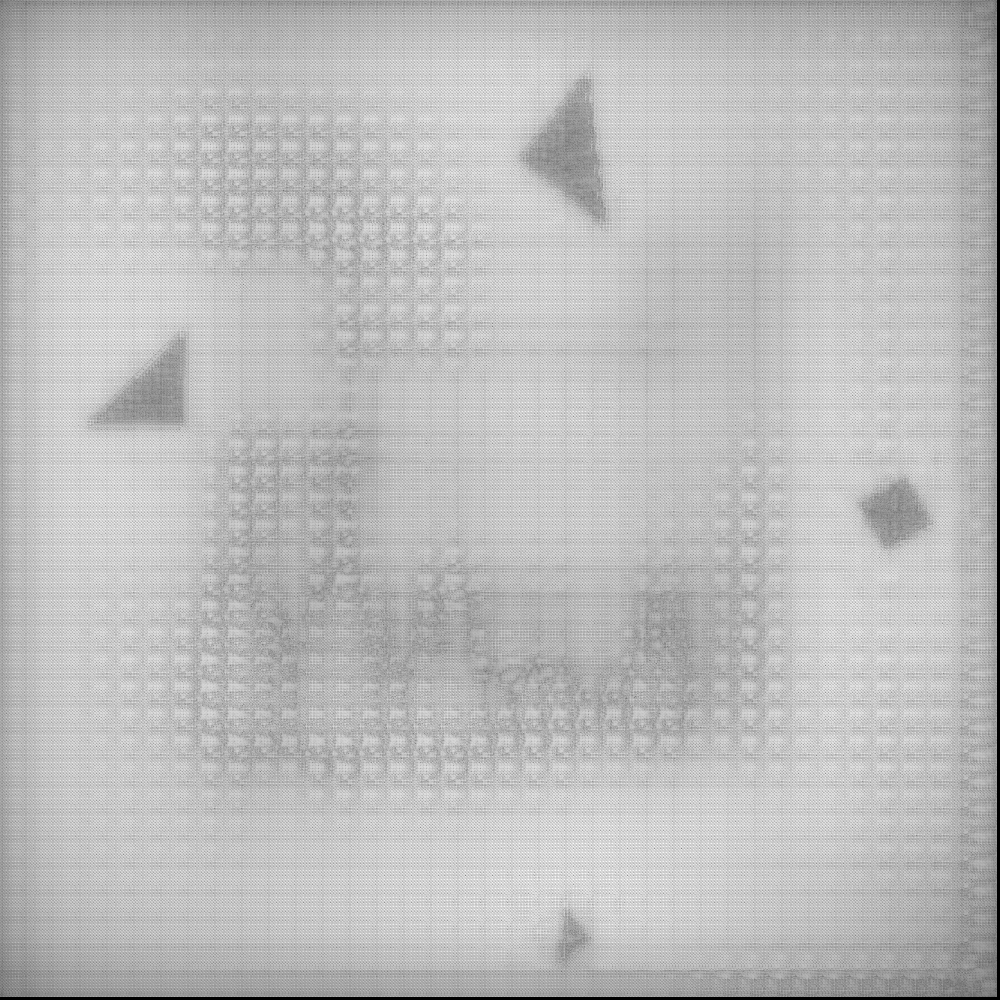
\includegraphics[width = 2.3in, height = 2.3in]{Counting/LaTeX/figures/putasideall/nolimitscaleresamplingoptiondifferentactivationnetworkputaside/image1/saliency.png}   & 
\includegraphics[width = 2.3in, height = 2.3in]{Counting/LaTeX/figures/putasideall/nolimitscaleresamplingoptiondifferentactivationnetworkputaside/image2/saliency.png} \\
            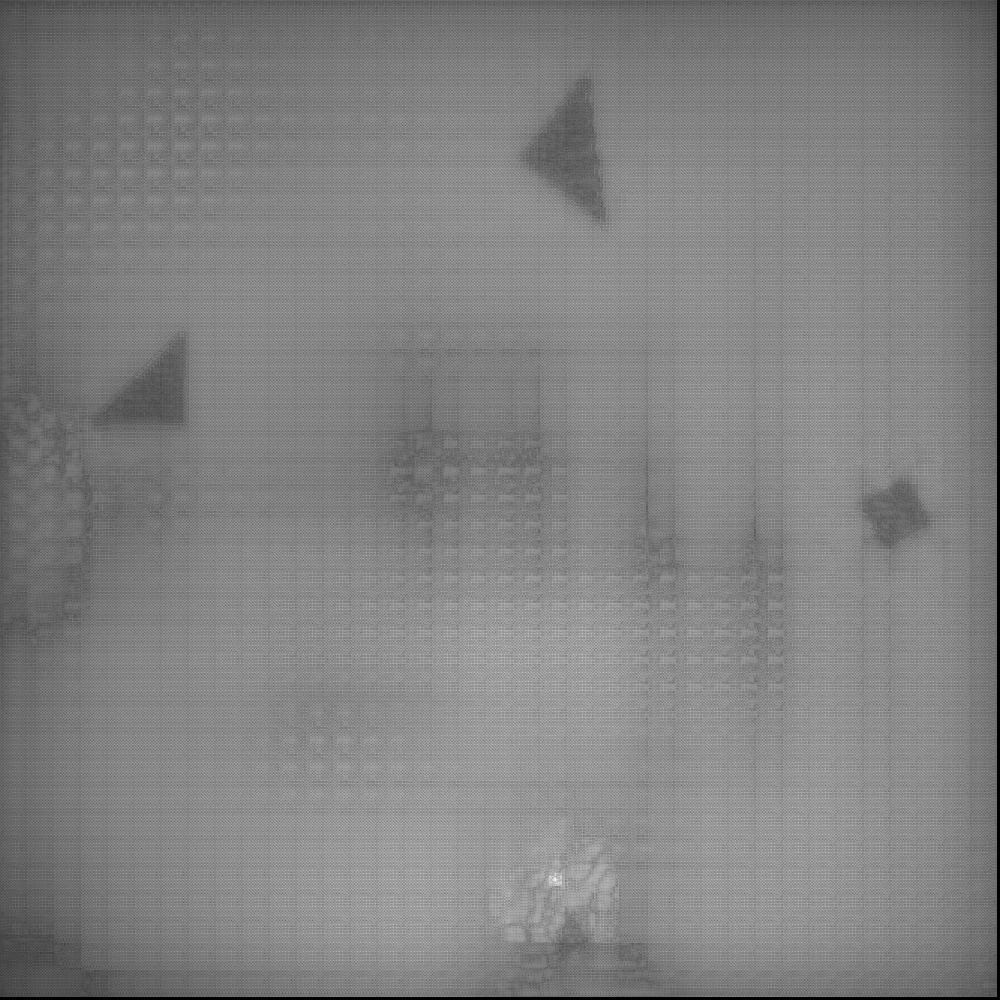
\includegraphics[width = 2.3in, height = 2.3in]{Counting/LaTeX/figures/putasideall/nolimitscaleresamplingoptiondifferentactivationnetworkputaside/image1/1-saliency.png}   & 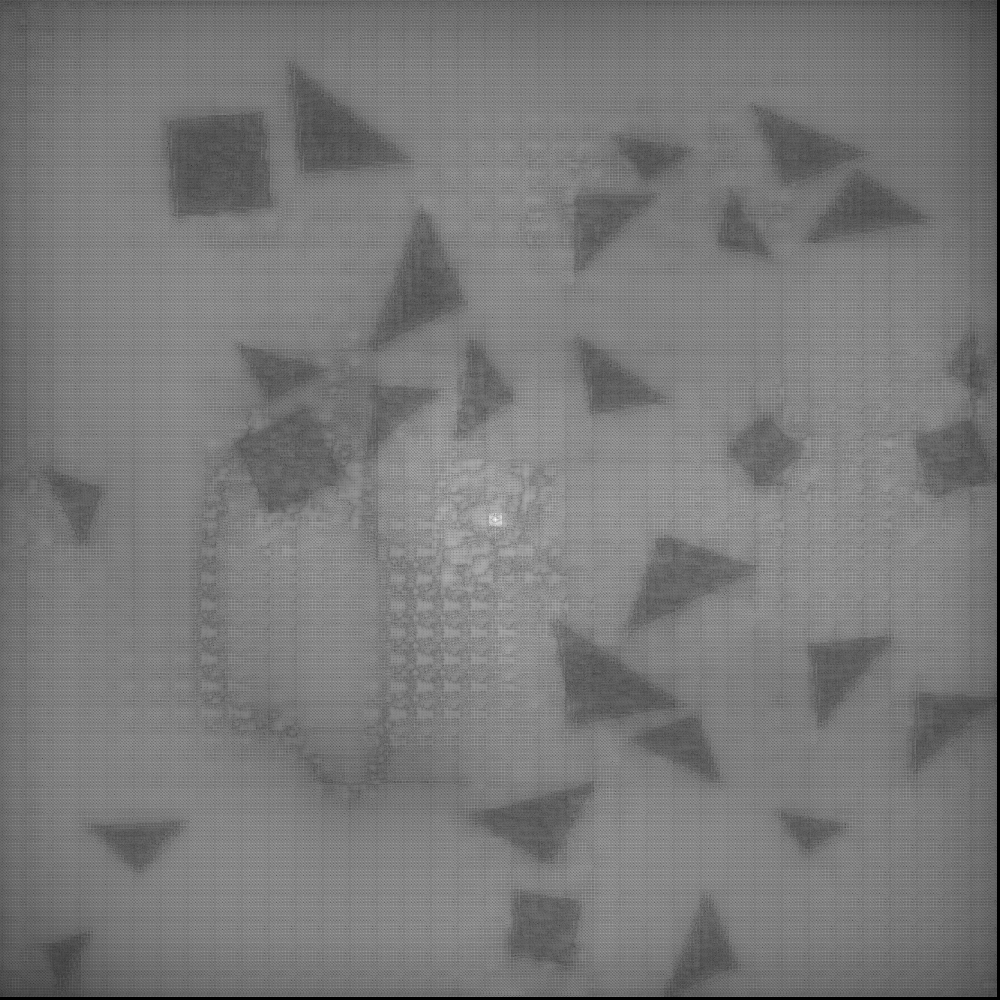
\includegraphics[width = 2.3in, height = 2.3in]{Counting/LaTeX/figures/putasideall/nolimitscaleresamplingoptiondifferentactivationnetworkputaside/image2/1-saliency.png} \\
            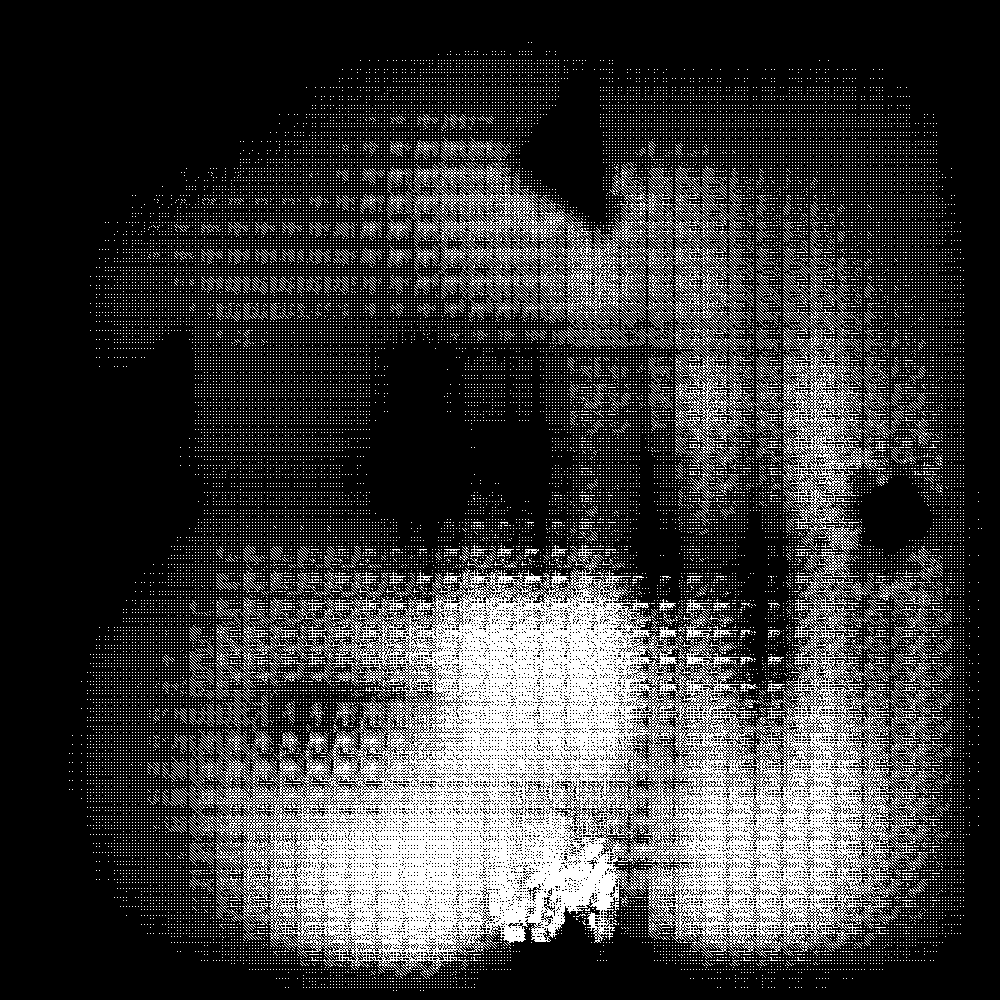
\includegraphics[width = 2.3in, height = 2.3in]{Counting/LaTeX/figures/putasideall/nolimitscaleresamplingoptiondifferentactivationnetworkputaside/image1/1.png} & 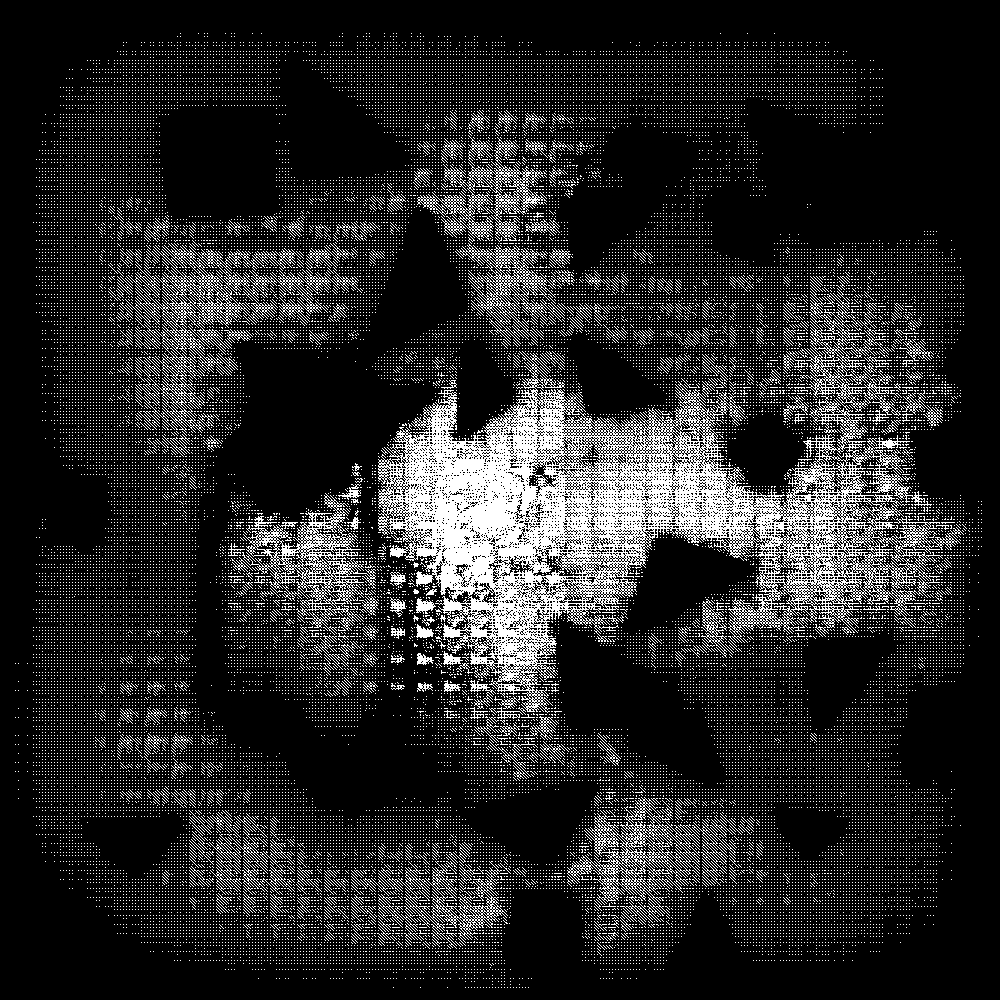
\includegraphics[width = 2.3in, height = 2.3in]{Counting/LaTeX/figures/putasideall/nolimitscaleresamplingoptiondifferentactivationnetworkputaside/image2/1.png}
        \end{tabular}
    \end{center}
    \caption{The first row shows saliency maps for two images, the second row shows the connection
             strength between the most salient pixel and others, and the third row are the pixels
             that ``qualify'' as being part of a shape}
    \label{badsaliency}
\end{figure}





Further tweaks need to address the problem discussed in section \ref{algorithm}. Regarding the most
salient pixels being between shapes, it may be necessary to modify the loss function from which to
backpropagate. Candidates would need to encode encouraging strong gradients that \textit{only}
relate to decreasing the count by one. Another option is to threshold the first derivative saliency
from above. As a result, errant pixels in the gap between shapes with large saliency would not be
considered. Further, as stated previously, automatic determination of both thresholds would be
substantially better than manual settings. This would become even more crucial when tackling
real-world issues. An alternative solution may be to use K-means to group low, medium and high
saliency pixels. The idea is that we would only stick with the medium-saliency pixels as the high
saliency group would have many pixels that may change the count too much; rejecting those with low
saliency values was justified previously. One may need to consider the distance metric to be used;
for example, high saliency pixels may be distributed in an exponential fashion, so normal Euclidean
distance would leave many undesired saliencies in the acceptable group.

Further, it is important to point out that real-world circumstances may actually provide
\textit{better, more reliable} saliency values. Counting shapes may have a significant flaw, which
is that ordinary, monocolor shapes really don't have many features outside of their edges and
corners\footnote{David Crandall reminded me about corners possibly being important.}. If there are
features that are internal to the object, it may result in cleaner saliency values that are focused
on the object itself. However, it is also possible that the network learns to identify one component
that many objects in the image share, and, as a result, its children pixels do not span the object
entirely, making bounding box prediction problematic.

% ^^^edit2^^^ said that the first quotation mark wasn't the correct kind, which made me realize that
% I didn't use the proper `` and '', so this was changed.
Our code and models can be found in the ``Counting'' folder at \cite{mycode}.




\chapter{Representation in the Face of Adversaries}

\section{Predecessors}

\subsection{\textit{Intriguing Properties of Neural Networks} (Szegedy et. al)}
The paper that truly brought to light the issue of adversarial attacks was
\cite{szegedy2014intriguing}. In this paper, they provide an optimization-based approach to
generating what are known as ``adversarial examples''. To do this, they trained multiple models with
fully-connected neurons on the MNIST training dataset\cite{lecun}. One of the networks was  an
autoencoder. After performing this task, they generated adversarial examples for the sake of
comparing the performance of the non-attacked network to the attacked network. In order to do this,
they used L-BFGS\cite{lbfgs} (modified to keep any changes within the $L_{\infty}$ norm) to try to
minimize the loss function, but with the target class being an incorrect class. They also made sure
that the predicted class of the modified image is indeed the class they were hoping to achieve, and
the modifications did not cause resulting input values to be less than zero or greater than one (the
bounds on the possible values in the image). This resulted in images (derived from the training set)
that visually still should not be misclassified, yet the neural network (and a few linear
regression-based models) misclassified them. In fact, they were able to get accuracy down to 0\%
using noise that one would not think could change the classifer's output. These kinds of corrupted
images were shown in their work, and are reproduced in Figure \ref{adversarialexamplespictures}.

\begin{figure}
    \begin{center}
        \begin{tabular}{c c}
            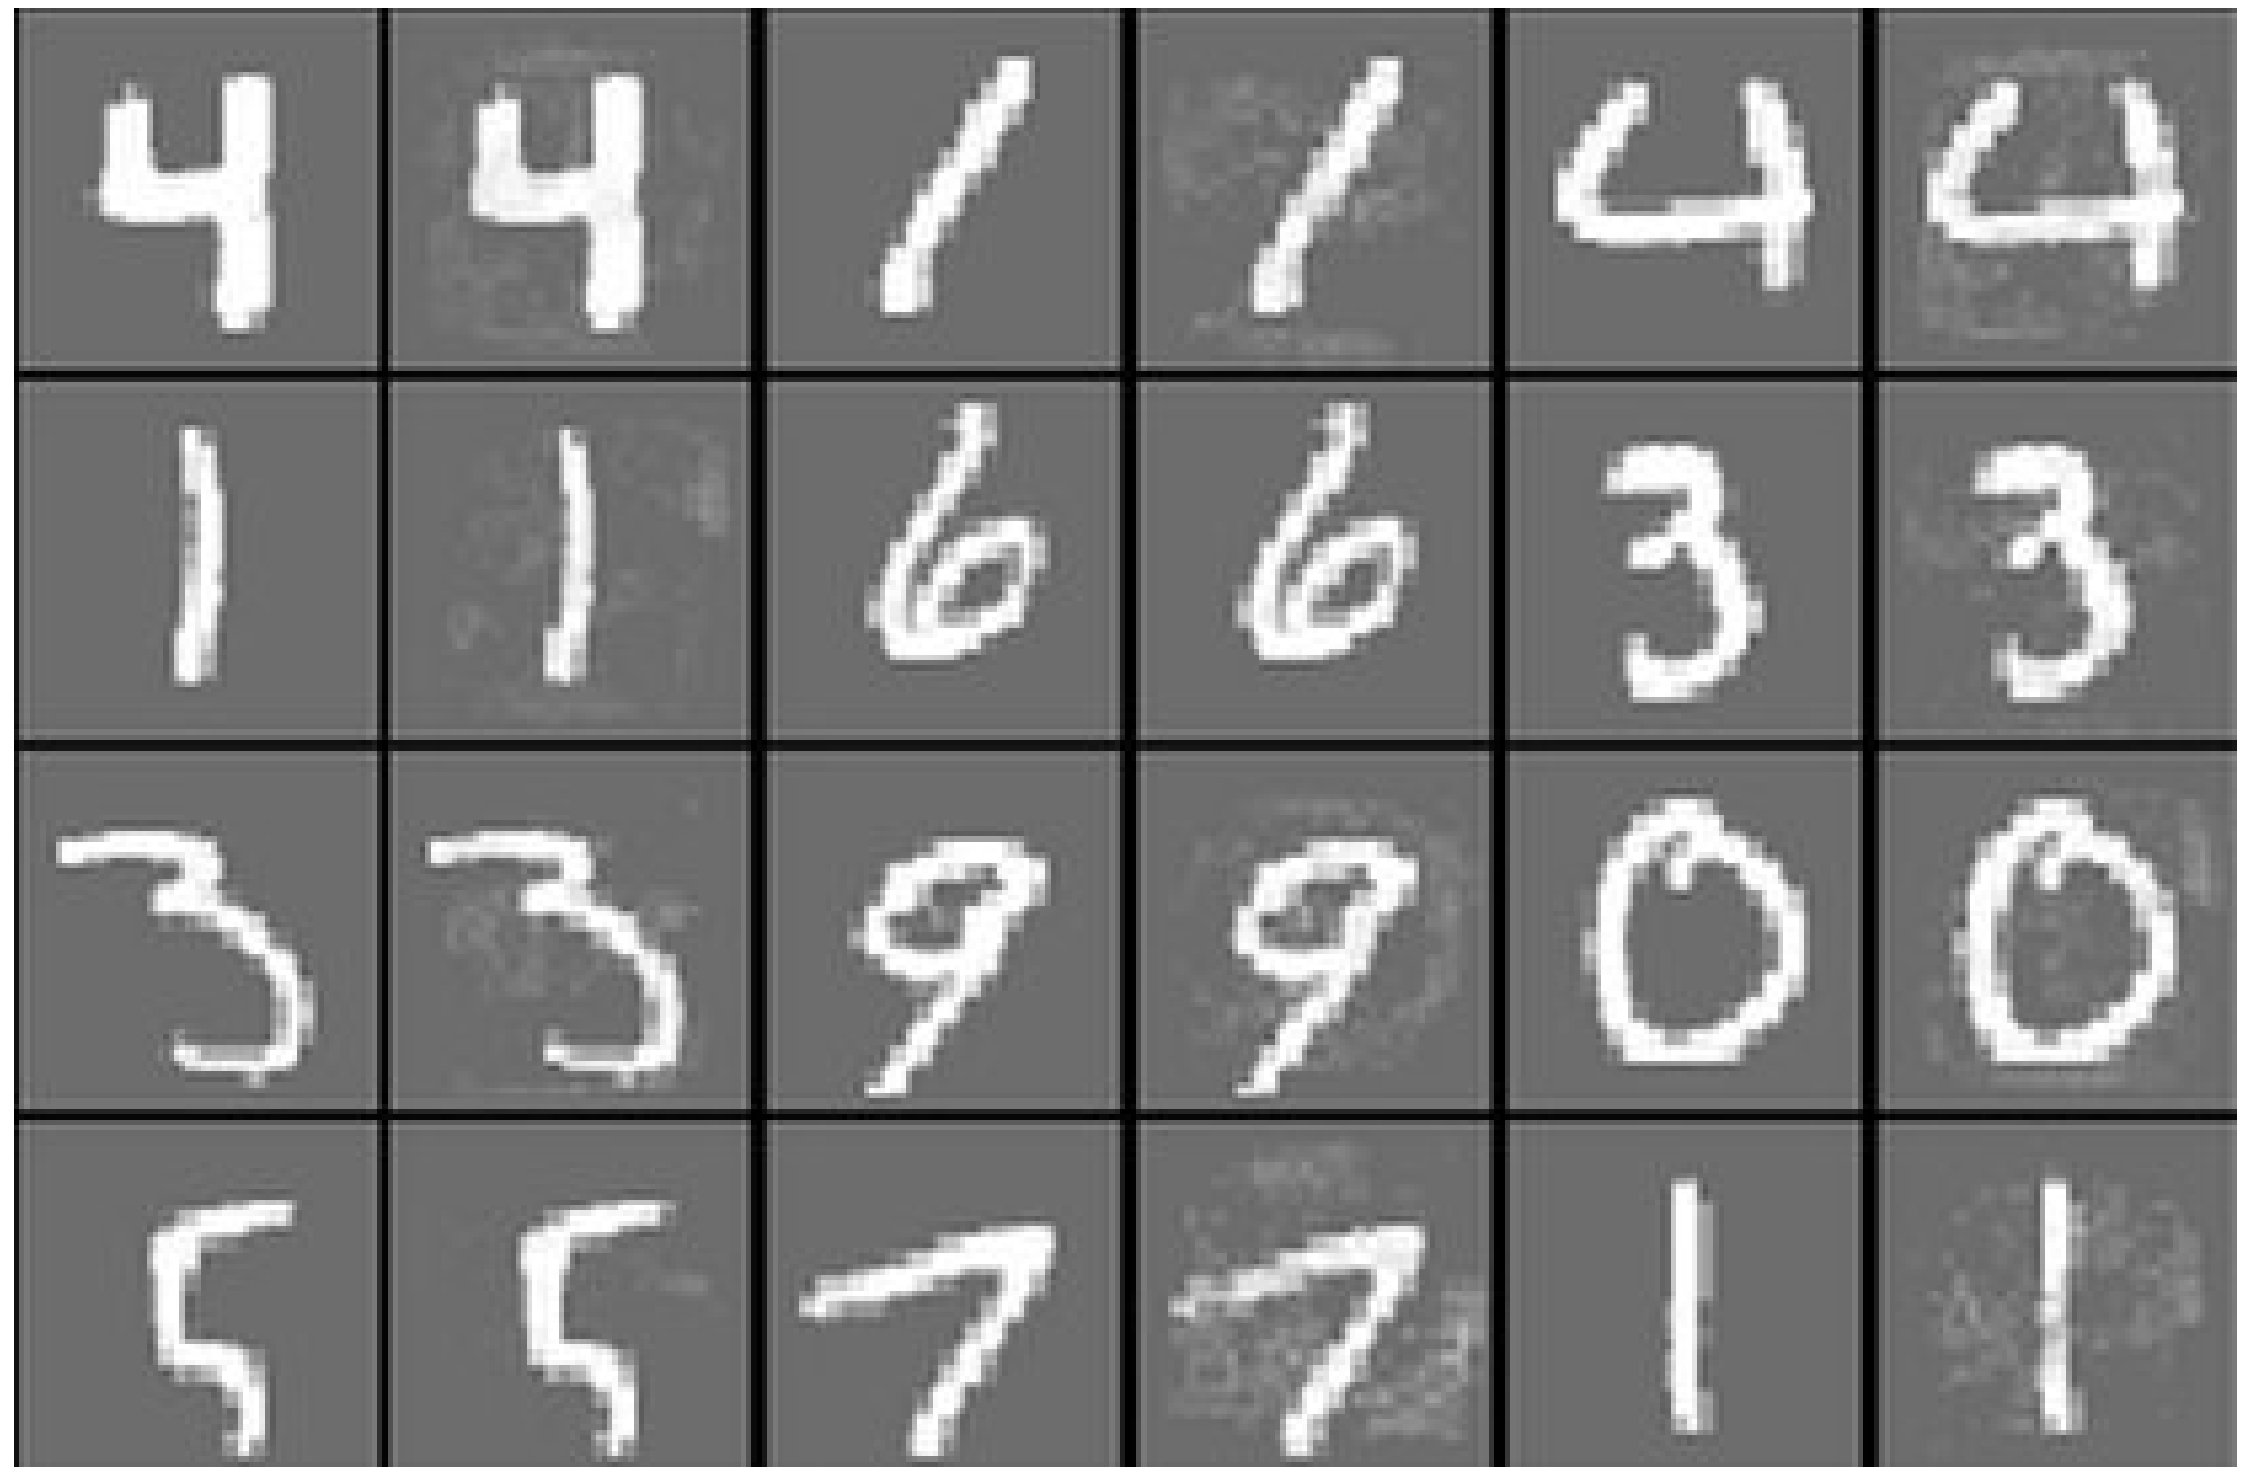
\includegraphics[width = 3in]{Friendly/LaTeX/figures/grid1.png} & 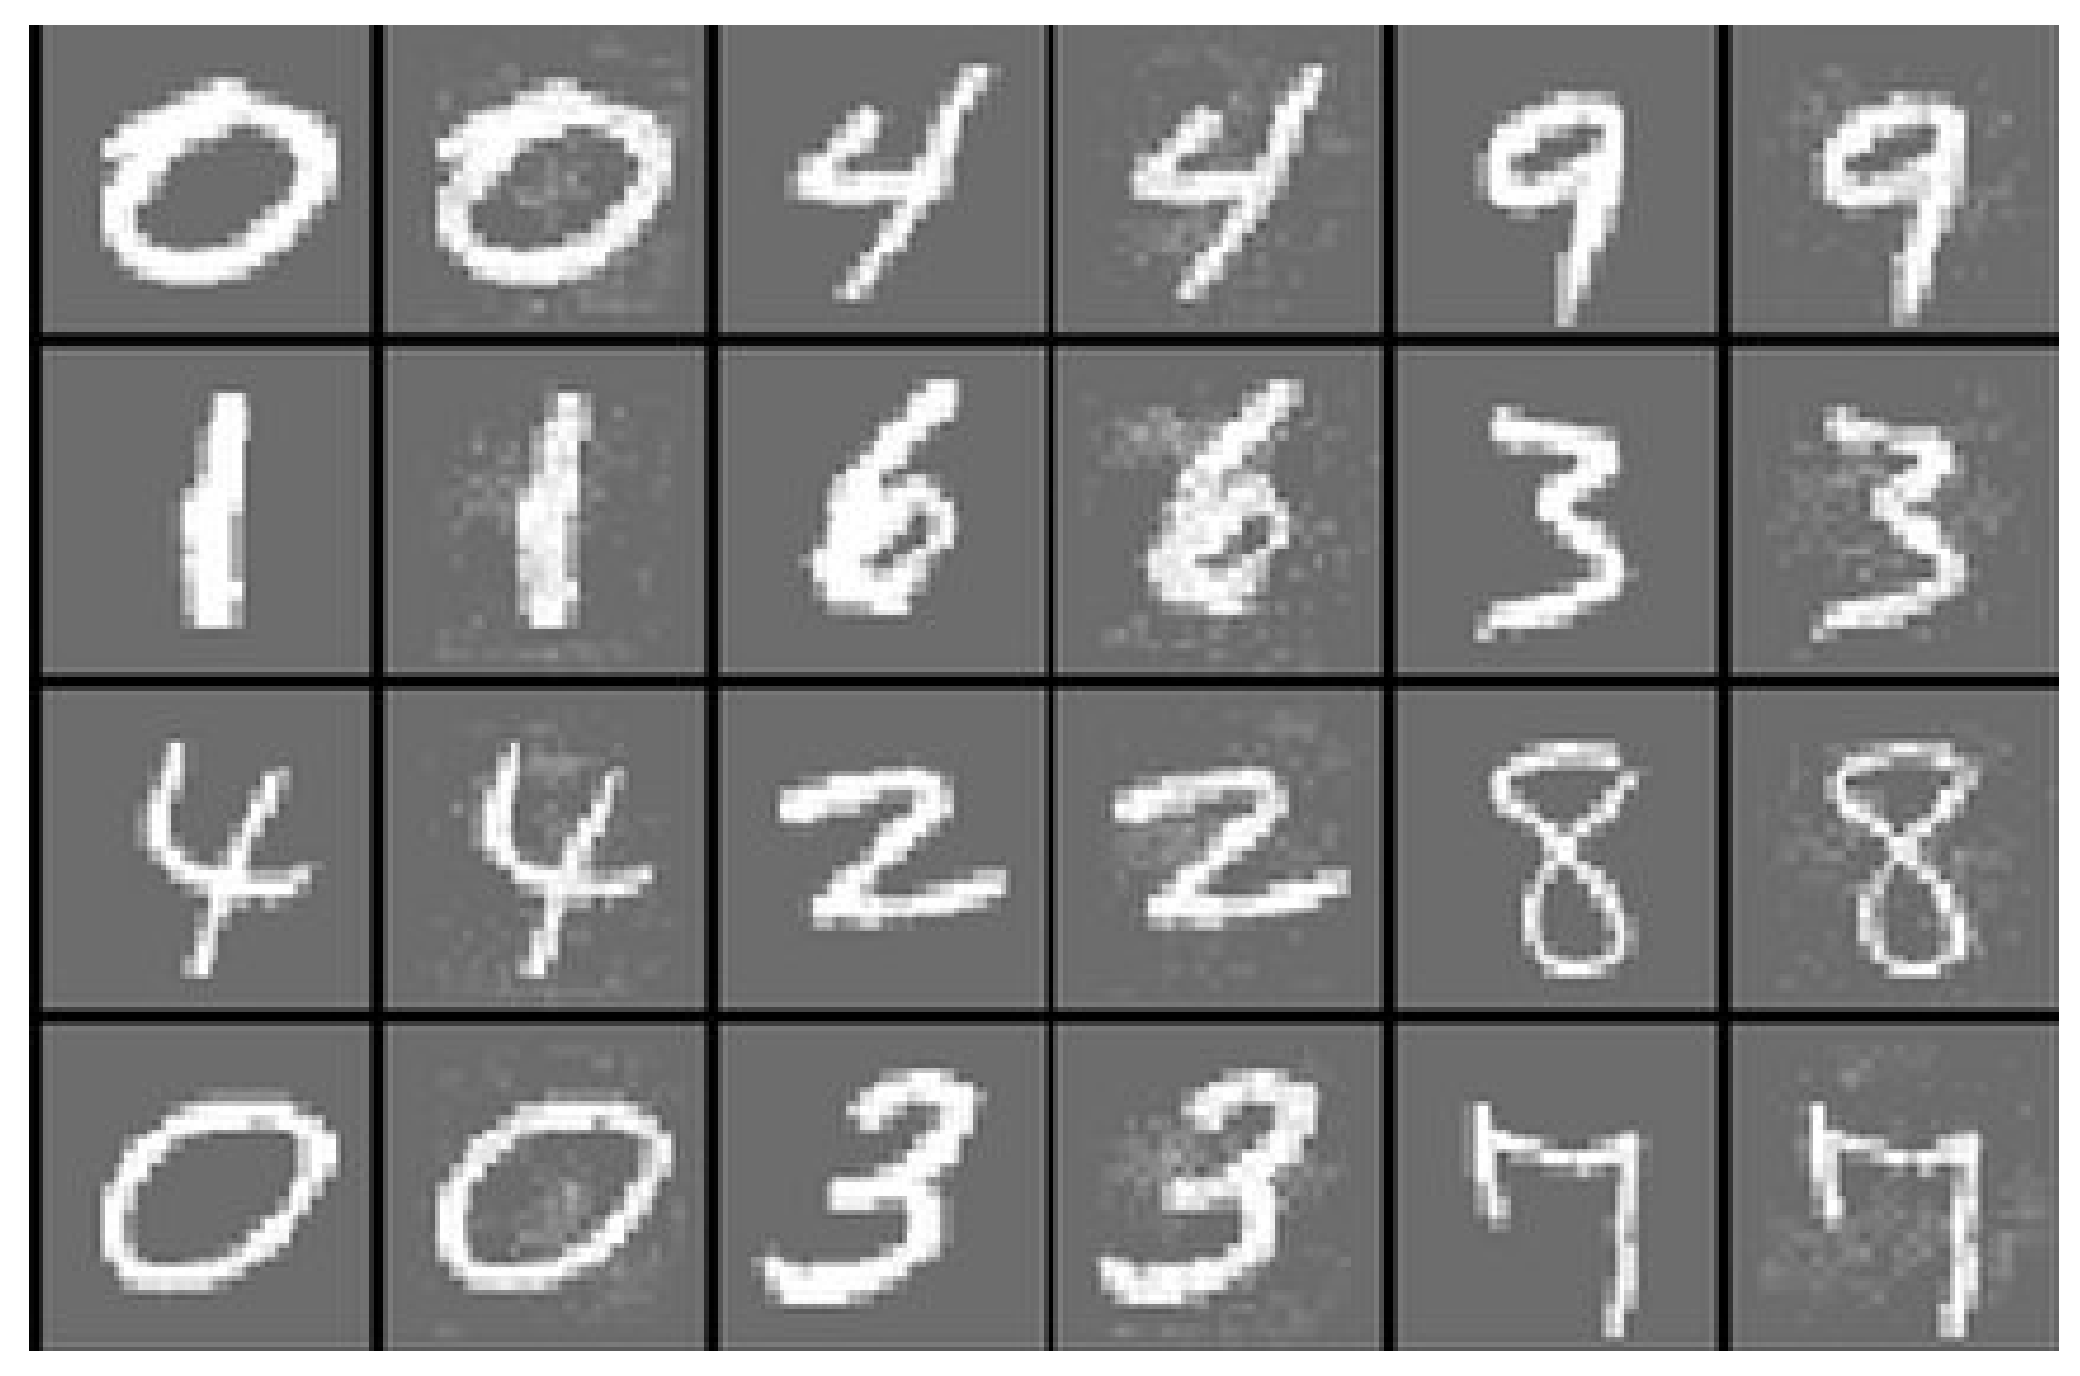
\includegraphics[width = 3in]{Friendly/LaTeX/figures/grid2.png}
        \end{tabular}
    \end{center}
    \caption{Adversarial images taken from ~\cite{szegedy2014intriguing}[figure 7] where the noisy
             images are the adversarial examples. See the figure of that paper for details about
             these images}
    \label{adversarialexamplespictures}
\end{figure}

They also tried to use these adversarial images from one model on the other models. They did this
for each model so that every model in the test was used to generate adversarial examples to be used
on the others. The error rate for the other models was substantially lower; however, the minimum
error rate (of all tests) was still a few times higher than data that had not been disturbed, with a
few error rates well over 70 percent. Further, to eliminate the possibility that this isn't a issue
of using the same dataset, one network was trained on a different subset of the MNIST dataset. For
the two that were trained on the opposing subset, one of them had a different number of neurons than
the other. They say these two differences were tested at once (with the different network) "to study
the cumulative effect of changing the hyperparameters and the training sets at the same
time"\cite{szegedy2014intriguing}[p.\ 8]. The results show that there is roughly an equivalent
contribution, between dataset and model setup, to error rate with sabotaged images at low
magnitudes. However, when they increased the magnitudes of the noise, the shared-training-scenario
dataset caused much more misclassification when compared to having the training sets be the same
when transferring in both directions between the different models.

The final part of the paper tried to analytically quantify the capability an adversarial sample has
to affect the network's ability to classify things correctly. They used an interesting technique of
a establishing series of derivative upper bounds that cascade through the network, resulting in a
cumulative upper bound.
\subsection{\textit{Explaining and Harnessing Adversarial Examples} (Goodfellow, Schlens, and Szegedy)}
\cite{szegedy2014intriguing} was shortly followed up by \cite{goodfellow2015explaining}, which
brought to light strong evidence that the cause of these adversarial examples is the linearity of
the models being used (this linearity turns out to be limited, as discussed in \ref{tdlmrtaa}).
Mathematically, they point to the dot product that occurs in typical neurons and how drastically it
can change when only small changes to the input vector in the dot product occur. Analytically, they
come to this conclusion by pointing out that an adversarial example with noise $\eta$ for original
image $x$ will end up in the dot product with weight vector $w$ (note: all symbols used here are
from the paper); further, we added this equation for clarity, but keeping $w$ transposed instead of
the input vector):

$$w^T(x + \eta)$$

After distribution, they point out that the second term in the resulting addition is $w^T\eta$, a
non-negligible value (due to the number of elements participating in the dot product). They
end up drawing this conclusion: the dot product determines the final activation value, so, under a
max-norm constraint, noise added to a many-element vector may not appear to be much from the
max-norm perspective, but actually \textit{is} from the dot product perspective.

They bring up other theories about these phenomena, including the idea that nonlinearities are
causing them and that ``adversarial examples finely tile space like the rational numbers among the
reals''\cite{goodfellow2015explaining}[p. 7]. To debunk the first notion, they developed their own
attack called the \textit{Fast Gradient Sign Method} (FGSM). This attack consists of optimizing an
image by stepping away from the minimum, as opposed to towards it (the latter is the case in
training, and the parameters being optimized are that of the network instead of the image). This
uses the gradient (w.r.t. the image) of the actual loss of the image and its ground truth. However,
a modification here is that the sign of the gradient, after being multiplied by an
intensity-controlling value called $\epsilon$, is used in place of the gradient itself.

The goal of FGSM is two-fold. First, this method quickly generates adversarial examples instead of
normal iterative optimization found in \cite{szegedy2014intriguing}, as they point out. They state
that this makes training with adversarial examples (in addition to the regular images) much faster.
The second reason for its existence is to prove that the attack space is a continuously linear
subspace.

One reason that they note is simply because increasingly larger magnitudes of $\epsilon$ result in
even higher confidence in the same wrong class. However, the series of pictures in figure
\ref{imagegrid} that shows a visualization of the examples at those $\epsilon$ values shows the vast
majority of misclassified images being what they call ``rubbish examples'', and it appears that they
use that term to describe significantly fewer samples in that image than we would. There are only a
handful of misclassified subimages in that figure that, in our opinion, are actually recognizable
enough to not be considered rubbish.

\begin{figure}[th]
    \begin{center}
        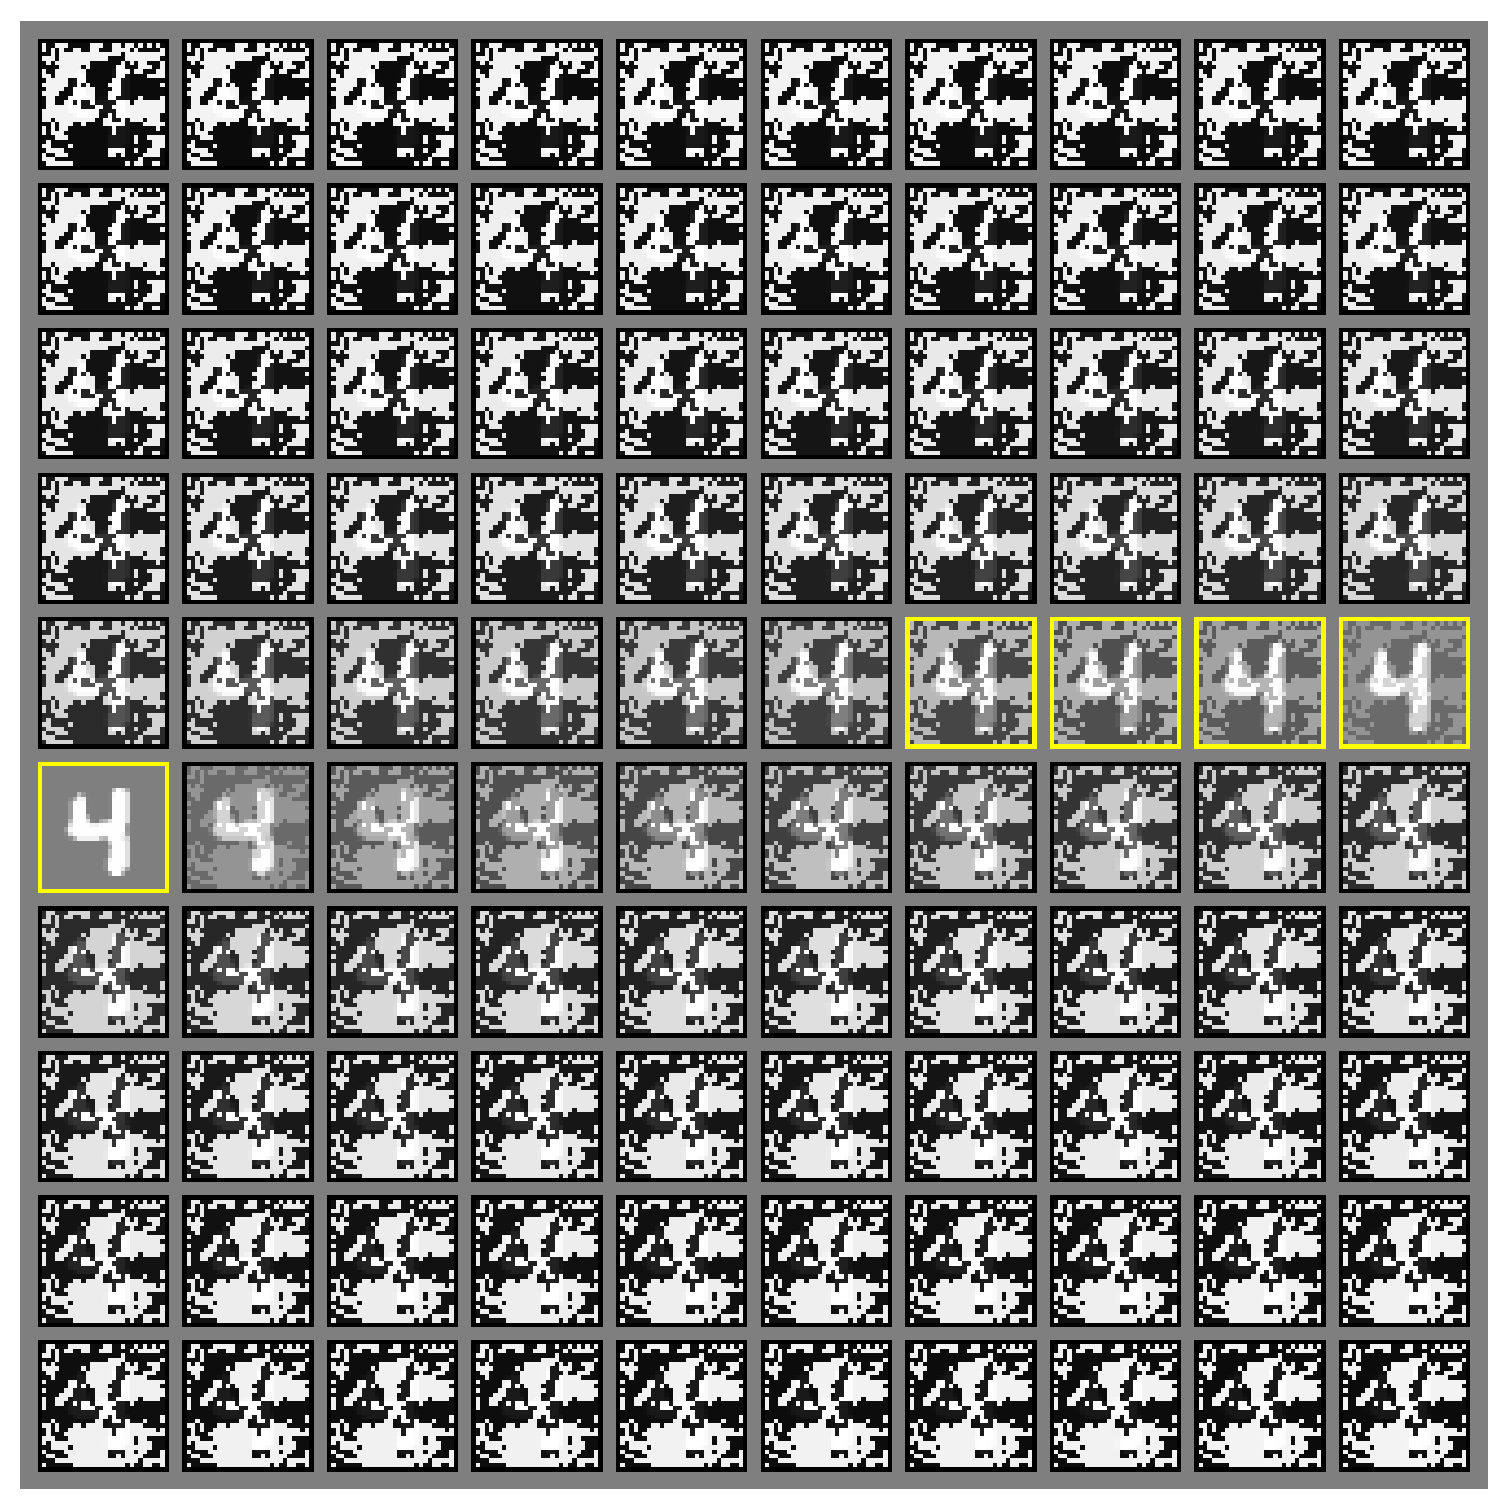
\includegraphics[width = 4in]{Friendly/LaTeX/figures/goodfellowdisagreement.png}
    \end{center}
    \caption{Part of figure 4 from \cite{goodfellow2015explaining}. The number of rubbish examples
             appears to be more than they indicate.}
    \label{imagegrid}
\end{figure}

A second thing that they point to is that adversarial examples created using a Radial Basis
Function-based network and a shallow neural network that uses Softmax (likely just on the logits of
the network) do not transfer as well to each other as the Softmax-based one does to a
Maxout~\cite{goodfellow2013maxout} network, which is more linear. A possibly important point to note
is that they state that the first network is ``shallow''\cite{goodfellow2015explaining}[p. 7], but
this author is not sure exactly what that means in the context of Maxout networks.
\subsection{\textit{Towards Deep Neural Network Architectures Robust to Adversarial Examples} (Gu and Rigazio)}
Prior to \cite{goodfellow2015explaining}, Shixiang Gu and Luca Rigazio, in \cite{gu2015deep}, made
an attempt at solving the adversarial example problem. They made two important contributions to this
field.

The first was addressing the natural intuition that one would try to use an autoencoder to return an
adversarial example to its clean state. Training of this autoencoder consisted of not just the
inputs being the modified images and the original (off of which the loss is calculated) but also the
non-modified image and the original. This was done to ensure that the autoencoder wouldn't
unnecessarily de-noise its input. This was a largely successful method, but it revealed a flaw of
using such techniques: this autoencoder is also a neural network, and it can also be attacked with
essentially the same success rate of just attacking the classifier. Even worse, they found that the
magnitude of this new noise was substantially \textit{smaller} than the original noise. Further,
they point out that ``[f]or any pre-processing, it is always possible to backpropagate the error
signal through the additional functions and find new adversarial examples...''\cite{gu2015deep}[p.
5], essentially eliminating any usefulness of any other solutions like their autoencoder, and
implying that differentiable methods of countering this noise, regardless if it is an autoencoder or
some other method, are included too. It is important to point out, however, that these autoencoders
are also linear neural networks, so it's possible that this mindset isn't valid for denoising
approaches that avoid the linearity issue discussed in \cite{goodfellow2015explaining}.

For their other contribution, they desired to introduce an additional penalty, during training, on
the magnitude of the gradient w.r.t the image. The idea behind this is that small changes to an
image should not escape the local, correctly-classified region created by training on the
non-adversarial example. However, they stated that they did not have the computational resources to
do this. Instead, for each layer, they penalized the 2-norm of the gradient from a layer's output
w.r.t.\ its successor, using the image as a predecessor to the first layer. These penalties were
added up per image (as in, the gradients penalized were obtained by backpropagating from the loss of
each image, not from the loss of each batch). Their results did show improvement, but not in a
significant way. One reason could be that the addition they tried does not obey the chain rule;
multiplying the norms may have made more sense to get the chain rule effect. However, a more
plausible explanation for this issue will be discussed later when we implement their ideal
full-gradient ourselves.
\subsection{\textit{Obfuscated Gradients Give a False Sense of Security: Circumventing Defenses to Adversarial Examples} (Athalye, Carlini, and Wagner)}
Unfortunately for the works that followed, \cite{athalye2018obfuscated}, for lack of a formal
descriptive phrase, ``rained on their parade''. They confront the idea of \textit{obfuscated
gradients} (credited to \cite{10.1145/3052973.3053009} by \cite{athalye2018obfuscated}), which they
explain is the scenario in which there are no gradients that can be used for a white-box attack. To
counter these defenses, to this author's best recollection, they employ two main methods,
\textit{Backward Pass Differentiable Approximation} and \textit{Expectation Over Transform} (the
latter is from \cite{athalye2018synthesizing}); for brevity, they use the acronyms \textit{BPDA} and
\textit{EOT}, so we will do the same for the same reason.

BDPA solves the issue where the gradients are not easy to retrieve. In this technique, the part of
the machine learning algorithm for which the gradients cannot be calculated is replaced by a
near-equivalent that has this property. However, this replacement only occurs when calculating
gradients. They imply that it is likely necessary to use some kind of running average of the
gradients used to generate the adversarial example when iterative methods are used; this is due to
the fact that one single gradient calculation would be an approximation given the different
function.

The next method, Expectation over Transform, finds the expectation of the gradient when any one of
many different operations may be used on the input at any forward pass before it goes into the
network. In the EOT paper~\cite{athalye2018synthesizing}, they highlight transformations such as
scaling, brightness modification, and rotations. In \cite{athalye2018obfuscated}, these
transformations take the form of anything non-deterministic that is done to the image for the
intentional or unintentional sake of defending the network. The idea is that the average gradient
will be a decent approximation to an adversarial gradient. It is not clear if the averaging only
occurs in an offline setting or if it occurs online as well (such as during gradient descent
optimization when creating the adversarial example). Further, in at least one case, the literal
average is not used; instead, it is a simple summation of gradients.

They find the vast majority of their attacks successful implying, if not outright saying, that
white-box attacks should not be the only metric by which a defense's effectiveness should be
evaluated. Further, they outline a series of steps that a researcher should take to properly state
the performance of their proposed defense; this appears to have mainly been done because most of the
defenses evaluated were overstating their technique's effectiveness. These steps are 1. ``[e]valuate
against adaptive attacks''\cite{athalye2018obfuscated}[§ 6], 2. "[m]ake specific, testable
claims"\cite{athalye2018obfuscated}[§ 6] and 3. "[d]efine a (realistic) threat
model"\cite{athalye2018obfuscated}[§ 6]. The last two are self-explanatory, and for the first,
``adaptive attacks'' appears to be described as ``[attacks] that [are] constructed after a defense
has been completely specified, where the adversary takes advantage of knowledge of the defense and
is only restricted by the threat model''~\cite{athalye2018obfuscated}[§ 6.3]. In this case, the
``threat model'' defines what the adversary knows. In \cite{athalye2018obfuscated}[§ 6.3], they
state that running the whole gamut of modern attacks would fit this definition.
\label{oggafsoscdtae}
\subsection{\textit{Towards Deep Learning Models Resistant to Adversarial Attacks} (Madry et. al)}
\label{tdlmrtaa}
\cite{madry2019deep}'s goal was to find both a defense and an attack mechanism that acted as some
kind of an upper bound for their respective roles, at least from the standpoint of noise being
within an $L_{\infty}$ norm set of boundaries. They proposed adversarial training (which is when the
network is trained on data that has been compromised) but a more advanced form of it. Adversarial
training has been tried previously (most prominently, and probably originally, in
\cite{goodfellow2015explaining}). However, as demonstrated in \cite{madry2019deep},
\cite{goodfellow2015explaining}'s procedure is not a sufficient procedure to ensure that one's model
can handle adversarial examples.

They start out their search by analytically encoding the adversarial training issue in the form of a
loss function that, when this function's value is reduced, is equivalent to min-max optimization.  In
this scenario, the ``max'' is the adversary maximizing the loss function, while the ``min'' is the
defender minimizing that maximum. The question they then pose is: what kind of adversary can
actually find something at least close to the maximum loss when generating an advesarial example? It
turns out that
\begin{enumerate}
    \item doing repeated FGSM~\cite{goodfellow2015explaining} steps a certain number of times on the
       respective output of the last step, clipping to be within the allowed ball of noise, and then
    \item trying that loop several times but starting at uniformly random locations within the $L_{inf}$
       ball of allowed noise around the image
\end{enumerate}
reveals that the set of images generated by this method has little variance in loss value. They
refer to this method as \textit{Projected Gradient Descent} (PGD). The conclusion that they draw is
that
\begin{quote}
    \textit{...our exploration with PGD does not preclude the existence of some
    isolated maxima with much larger function value. However, our experiments suggest that such
    better local maxima are hard to find with first order methods...}
    --~\cite{madry2019deep}[section 3.2]
\end{quote}
and that, as a result, PGD (with the aforementioned randomization and, to the best of this author's
understanding, choosing the best example out of all of them) likely gives us something close to the
best attack possible.

Assuming that their assumptions are correct, this conclusion (alongside other point(s) made in the
paper) completes the requirements needed to make adversarial training an effective way to thwart
attacks. In order to empirically prove that adversarial training with PGD actually works, they
tested three different things: a white-box attack and two black-box attacks, each of which were
% Including the chapter listed in ^^^cifarsite^^ may have been what [7ffa04, bottom] desires, so
% it is included to be safe
attempted using multiple attack methods, both on MNIST\cite{lecun} and CIFAR-10\cite{cifar}[ch. 3].
Both as a defense and as an attack, PGD dominated the other methods. For adversarial training, only
one random point was selected, with their reasoning appearing to be that successive epochs will not
change the model enough such that only attacking once per epoch over several epochs will result in
roughly the same adversarial examples being generated using the full PGD attack per example during
one epoch. In comparison to FGSM-based adversarial training (modified from
\cite{goodfellow2015explaining} by having the training set consist only of perturbed images), there
were many instances in which, from the white-box perspective, any sort of robustness completely or
almost completely disappeared when using the CIFAR-10 dataset. Black-box attacks caused a less
dramatic decrease in model performance, but it was still significant. White-box attacks on models
with PGD-based adversarial training were only mildly successful on MNIST using basically any attack;
however, for CIFAR, ``[t]he adversarial robustness of our network is significant, given the power of
iterative adversaries, but still far from satisfactory''~\cite{madry2019deep}[page 12], nowhere near
matching the MNIST network when attacked. Typically, attacking with PGD resulted in the lowest
scores, and PGD with multiple candidate adversarial examples per image proved to be the most
detrimental. There was only one scenario in which FGSM was more effective as an attacker, and that
was in a black-box setting with a model from a different paper, \cite{tramèr2017space}. To wrap up,
they conclude that attacks like FGSM are not adequate by pointing out~\cite{madry2019deep}[§ 6] that
the fact that adversarially-trained networks that use FGSM cannot resist PGD, and, in the same
section, point to \cite{tramèr2017space}\footnote{The author has not read this paper} as proof that
non-linear attacks may be more viable the further out the adversarial example is from the sample.

\subsection{\textit{Adversarial Logit Pairing} (Kannan, Kurakin, and Goodfellow)}
\cite{kannan2018adversarial} came up with the idea of \textit{Adversarial Logit Pairing} (ALP). This
method puts both images with and without the perturbation through the network, but, instead of just
making sure that the adversarial image predicts the same class as the normal one (a la
\cite{goodfellow2015explaining}), the $L_2$ distance between the logit outputs of both images is
also penalized. In the case of a batch of images, the average $L_2$ norm is used.

They also attempted \textit{Clean Logit Pairing} (CLP) which involves no adversarial examples.
Instead, they did the same logit penalty between pairs of undisturbed images in the batch, but did
not do adversarial training. Again, this penalty is averaged over every image in the batch. They
point out that the effect of this is that the logits for each image will be more even due to the
fact that the other image probably has substantially different logits, so the penalty will bring the
two logits together. Because of this, they also tried a technique called \textit{Logit Squeezing}.
If the aforementioned cause of the effectiveness of Clean Logit Pairing is what is happening, then
it may make sense to just penalize the norm of the logits of each image (instead of the distance
between two different images). It is not stated, but each of these penalties (one per image) are
probably also averaged as in the previous methods.

When compared to a modified version of the PGD defense that originated in \cite{madry2019deep}, ALP
ended up modestly beating PGD against both white and black box (transfer) attacks using PGD on
MNIST\cite{lecun} and Street View House Numbers (SVHN)\cite{yuval}, and only lost by a small amount
when testing clean examples from SVHN. It also performed best against other defenses on tests on
ImageNet\cite{ILSVRC15}, both black-box and white-box, while non-adversarial performance remained on
par with the PGD-based defense. Both CLP and Logit Squeezing were as good from a white-box
perspective (although not quite good as ALP), and was comparable in other contexts.


\subsection{\textit{Ensemble Adversarial Training: Attacks and Defenses} (Tramèr et. al)}
\cite{tramèr2020ensemble} addressed the issue of black-box attacks. They found that the testing
regime used previously did not adequately assess whether adversarially trained models can handle
black-box adversarial examples in general. Specifically, they found that the linear black-box
attacks used (for example, FGSM\cite{goodfellow2015explaining}) were not good at reaching the
maximum in the min-max problem discussed in \cite{madry2019deep}, and that white box attacks turn
out to be not as good as black-box attacks on models that have been trained with first-order, single
step attacks. Further, it is possible that white-box attacks on these adversarially trained models
transfer poorly when used as part of a black-box attack on \textit{non-adversarial} models.

They came to these conclusions first by probing the loss function space with respect to a
two-dimensional subspace whose axes are essentially the sign of the gradient and a vector
perpendicular to it (likely inspired by \cite{goodfellow2015explaining}) scaled by increasing
adversarial perturbation magnitudes. At each point, two noise vectors generated from the first and
second magnitudes multiplied by the sign of the gradient and its orthogonal counterpart,
respectively, were added to the non-adversarial example (we will call these scaled vectors $a$ and
$b$, again, respectively). This generated a three-dimensional map, with the $z$ axis representing
the loss at the adversarial example represented by the point generated from the addition of $a$,
$b$, and the original image (axes represented the $L_{\infty}$ magnitude of $a$ and $b$). See figure
\ref{badgradients} for an example of a plot. They point out that the gradient at small perturbation values
points in a drastically different direction compared to the direction that would lead to the largest
increase in loss. They state that this explains both why white-box attacks on the aforementioned
adversarially-trained models do not work well on both the adversarially-trained and
non-adversarially trained models: this gradient does not represent the most effective direction for
ascent. Therefore, testing in the signed direction gives a false sense of security w.r.t. the
defended model, and these new images also, as a result, do not perform well as a black-box attack
against undefended ones. They call this phenomenon \textit{gradient masking}.
\begin{figure}[th]
    \begin{center}
        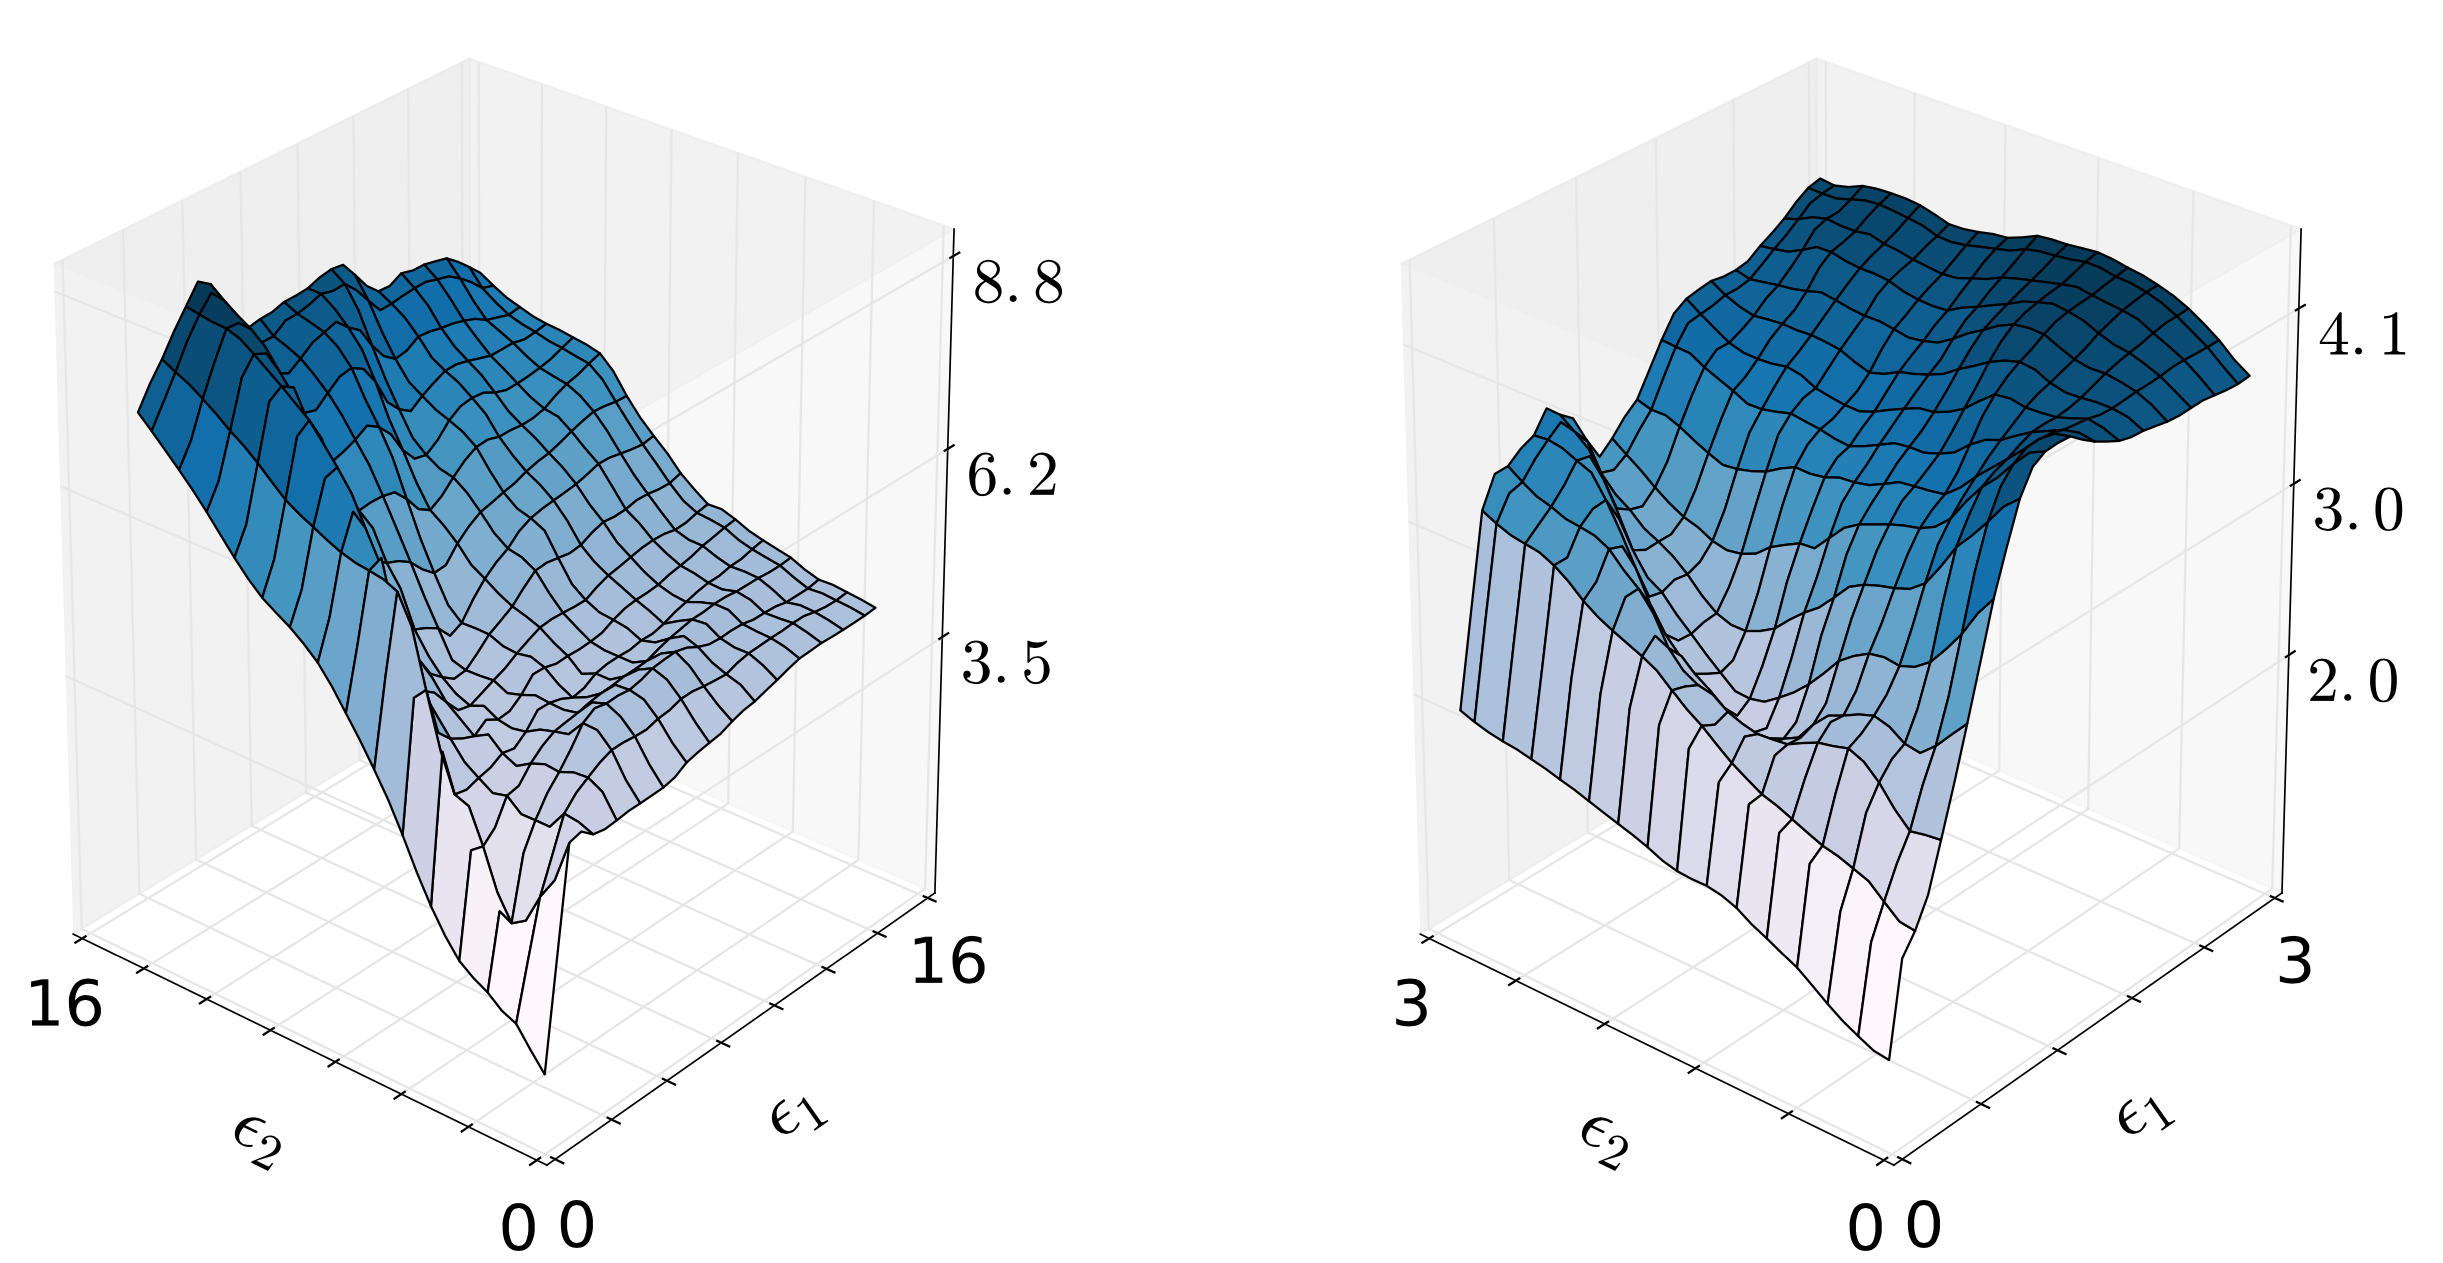
\includegraphics[width = \linewidth]{Friendly/LaTeX/figures/maskinggraphs.png}
        \caption{An example of gradient masking. The gradients in the data point's immediate
                 vicinity point one direction, while the actual maximizer is in the other direction.
                 Image is a snapshot from \cite{tramèr2020ensemble}[figure 4].}
        \label{badgradients}
    \end{center}
\end{figure}

To tackle this issue, they introduced \textit{Ensemble Adversarial Training}. In this technique,
not only do they train on white-box adversarial examples, but they also incorporate black-box
examples generated from non-adversarially-trained models. Each model contributed the same number
of adversarial examples, but only one model's adversarial examples were used each iteration. It
appears that only adversarial examples were in the training set. They found that this defense had
much better black-box resistance, and it eliminated cases in which the black-box attack was better
than white-box.

\section{Defense Proposals}

\subsection{Gradient Magnitude Reduction}
\label{gradientmagnitudereduction}
One solution to the adversarial examples problem is a simple and intuitive one: to penalize the
gradient with respect to the image. As stated in the literature review, this was proposed by
\cite{gu2015deep} (however, we independently developed it). To see why this makes sense, consider
the fundamental situation when it comes to adversarial examples: as \cite{goodfellow2015explaining}
states, dot products in deep learning can have \textit{many} terms. If this is unavoidable (more
on that later in other proposed defenses), then all we can do is to reduce the importance of each
pixel/subpixel, which can be seen as penalizing the gradient w.r.t. the (sub)pixels.

How to do this is not necessarily straightforward. For starters, we could penalize its norm. Which
norm to use may matter, but, in our implementation of this technique, we stuck with a normal 2-norm.
The calculation of the loss comes in two steps. The first step is do normal backpropagation towards
the image in order to get the gradient with respect to the image. The norm is then calculated, and
added to the normal loss term. Backpropagation occurs from there, which requires calculating the
``second derivative'' of the gradient (we use the derivative of the norm as the the gradient is a
vector and, therefore, its gradient is not well-defined). However, our choice of activation
function(s) may be problematic if they are not smooth (for example, the
ReLU\cite{pmlr-v15-glorot11a} activation function, which we found to be
problematic)\footnote{Double-checked by Stefan Lee}. To see why let us look at the ReLU activation
function. ReLU is specified as
\[
    \begin{cases}p & \text{for }p > 0 \\ 0 & \text{otherwise}\end{cases}
\]
where $p$ is the activation potential coming into the activation function. On one side of this
piecewise function, the derivative is always $0$, and on the other side, it is always $1$. It is
plain to see, then, that the second derivative will be zero everywhere, thus providing no utility when
it comes to gradient descent. This is a flaw in the nature of its linear, piecewise behavior;
mathematically, the second derivative does \textit{approximately} exist in the form of the
derivative of the SoftPlus~\cite{NIPS2000_44968aec} function. As a result (see § \ref{detectingshapes}), the image's
second derivative is zero. This is the case if we ignore the loss function, as one thing to consider
is the loss function's effect on the second derivative. Here, we can run into some trouble in our
hypothesis. Considering that using a smooth non-linear loss function $L$ is extremely common (for
example, mean squared error), there \textit{does} exist a non-zero second derivative for it. When
applying the product rule in this situation, for neural network $f$, we get
\[
    \frac{\partial}{\partial a} \left[ \frac{\partial L}{\partial f} \cdot \frac{\partial f}{\partial a} \right]
\]
as one of the terms in the product rule. This is non-zero (as our only hope of this being zero is if
the \textit{derivative} of the network output is zero). So, it \textit{is} possible to get some
second derivative out of a ReLU-based network (or any piecewise linear network, for that matter).
However, for our experiments, smooth functions were used to be more mathematically sound and to be
more sure that we have gotten closer to exhausting ways in which this method can go wrong.

Following \cite{goodfellow2015explaining}, we backpropagate from the correct class's loss. We will
call this method \textit{Gradient Magnitude Reduction} (GMR).

\subsection{Elastic Sigmoid}
A simple modification to penalizing the gradient is that, while doing so can change the weights, a
sigmoid function's derivative formulation cannot. Therefore, it make make sense to modify the
sigmoid activation function so that this is possible. There are many ways to do this: essentially,
one could enumerate all different combinations of sigmoid and some learnable parameter. One simple
use case for such a parameter is to multiply the activation potential by a scalar parameter $s$. The
reason why this can help change the layer's derivative is very simple: given the chain rule, the
derivative w.r.t. the potential $d$ (for ``dot product'') for the sigmoid activation function is
\begin{gather}
    \frac{\partial \text{sigmoid}(d)}{\partial d}
    = \frac{\partial}{\partial d} \frac{1}{1 + e^{-d}} \notag \\[10pt]
    = - \frac{1}{(1 + e^{-d})^2} \frac{\partial}{\partial d} e^{-d} \label{etothe} \\[10pt]
    = - \frac{1}{(1 + e^{-d})^2} e^{-d} \frac{\partial}{\partial d} (-d)
    = - \frac{1}{(1 + e^{-d})^2} e^{-d} (-1) \notag
\end{gather}
When we add in $s$, (\ref{etothe}) (and the rest of the derivative) becomes
\[
    - \frac{1}{(1 + e^{-sd})^2} \frac{\partial}{\partial d} e^{-sd}
    = - \frac{1}{(1 + e^{-sd})^2} e^{-sd} \frac{\partial}{\partial d} (-sd)
    = - \frac{1}{(1 + e^{-sd})^2} e^{-sd} (-s)
\]
As you can see, $s$ has a direct effect on the derivative of this new sigmoid function. If this is a
learnable parameter, decreasing $\left| s \right|$ through gradient descent will help with decreasing the norm of
the gradient. We call this new activation the \textit{Elastic Sigmoid}.

Note that there are nice properties in both directions in which the magnitude of $s$ can change. If
said magnitude gets smaller, we get the aforementioned effect. However, it is possible that it
becomes large if activation potentials never end up close to the origin. This is because, as $s$
increases in magnitude, the sigmoid tightens up to approximate the step function (or the
flipped-around-the-y-axis version of it caused by $s < 0$), exploiting the flatness of the step
function as long as the potentials end up far from the d-axis origin.

Another decision to make is whether or not there should be an $s$ for each neuron in the layer. This
obviously allows more flexibility if one neuron could benefit from a differently shaped Elastic Sigmoid
compared to another. We just use a single $s$ for the layer's activation due to time constraints.

\subsection{Pairwise Difference}
The next defensive structure we introduce is partially in response to the claim in
\cite{goodfellow2015explaining} about dot products wildly changing as a result of how many
components are multiplied within it. Further, it is ``inspired'' (in the loosest sense,
authoritatively speaking) by this author's very unscientific and personal experience when trying to
decipher hard-to-understand objects, visually speaking.

Let's say that we have a group of pixels for which we need to decipher what it represents. In this
case, the group takes on some kind of noise which makes it hard to recognize, yet the general themes
are still contained within the group (for example, it might be a very dark patch that needs careful
examinations of the relationship between connected components within it). Personally, the author
tries to find these connected components and perform the comparison. So, with that in mind, we
extend this technique to the deep learning case.

Inspired by convolutional neural networks, we take adjacent patches of pixels, and, in order to
approximate the connected-components analogy, we simply compare each pixel (or in the three-channel
case, subpixel, which we will refer to from here on) to every other within the patch. The way we
chose to compare subpixels is via a modification of the Distance Matrix\cite{wikipediadm}. Instead
of squaring the difference between subpixel values, we do not square at all. The reason for this is
simple: in the standard image processing case, distance would result in the same output when one
subpixel is less than or greater than the other used in the comparison. For this use case, that is
not necessarily ideal: if one pair is the inverted version of another within the image, they would
get the same distance value, but the inversion should really be considered a different relationship.

In mathematical terms, what follows is the definition of the difference matrix, $D$. Each subpixel
at position $j$ in the vector $\mathbf{v}$ that holds every element in the patch is subtracted from
element $i$ from that same vector. This creates the element $D_{ij}$; in other words, the index of
the subpixel from which element $j$ is being subtracted is $i$. Again, notice that this is derived
from the definition of the distance matrix, except in that case, $D_{ij}$ is actually $\left(
\mathbf{v}_i - \mathbf{v}_j \right)^2$. See figure \ref{pairwisedepiction} for a graphical view of
this neuron's layout.

\begin{figure}
    \begin{center}
        \begin{tabular}{c c c}
            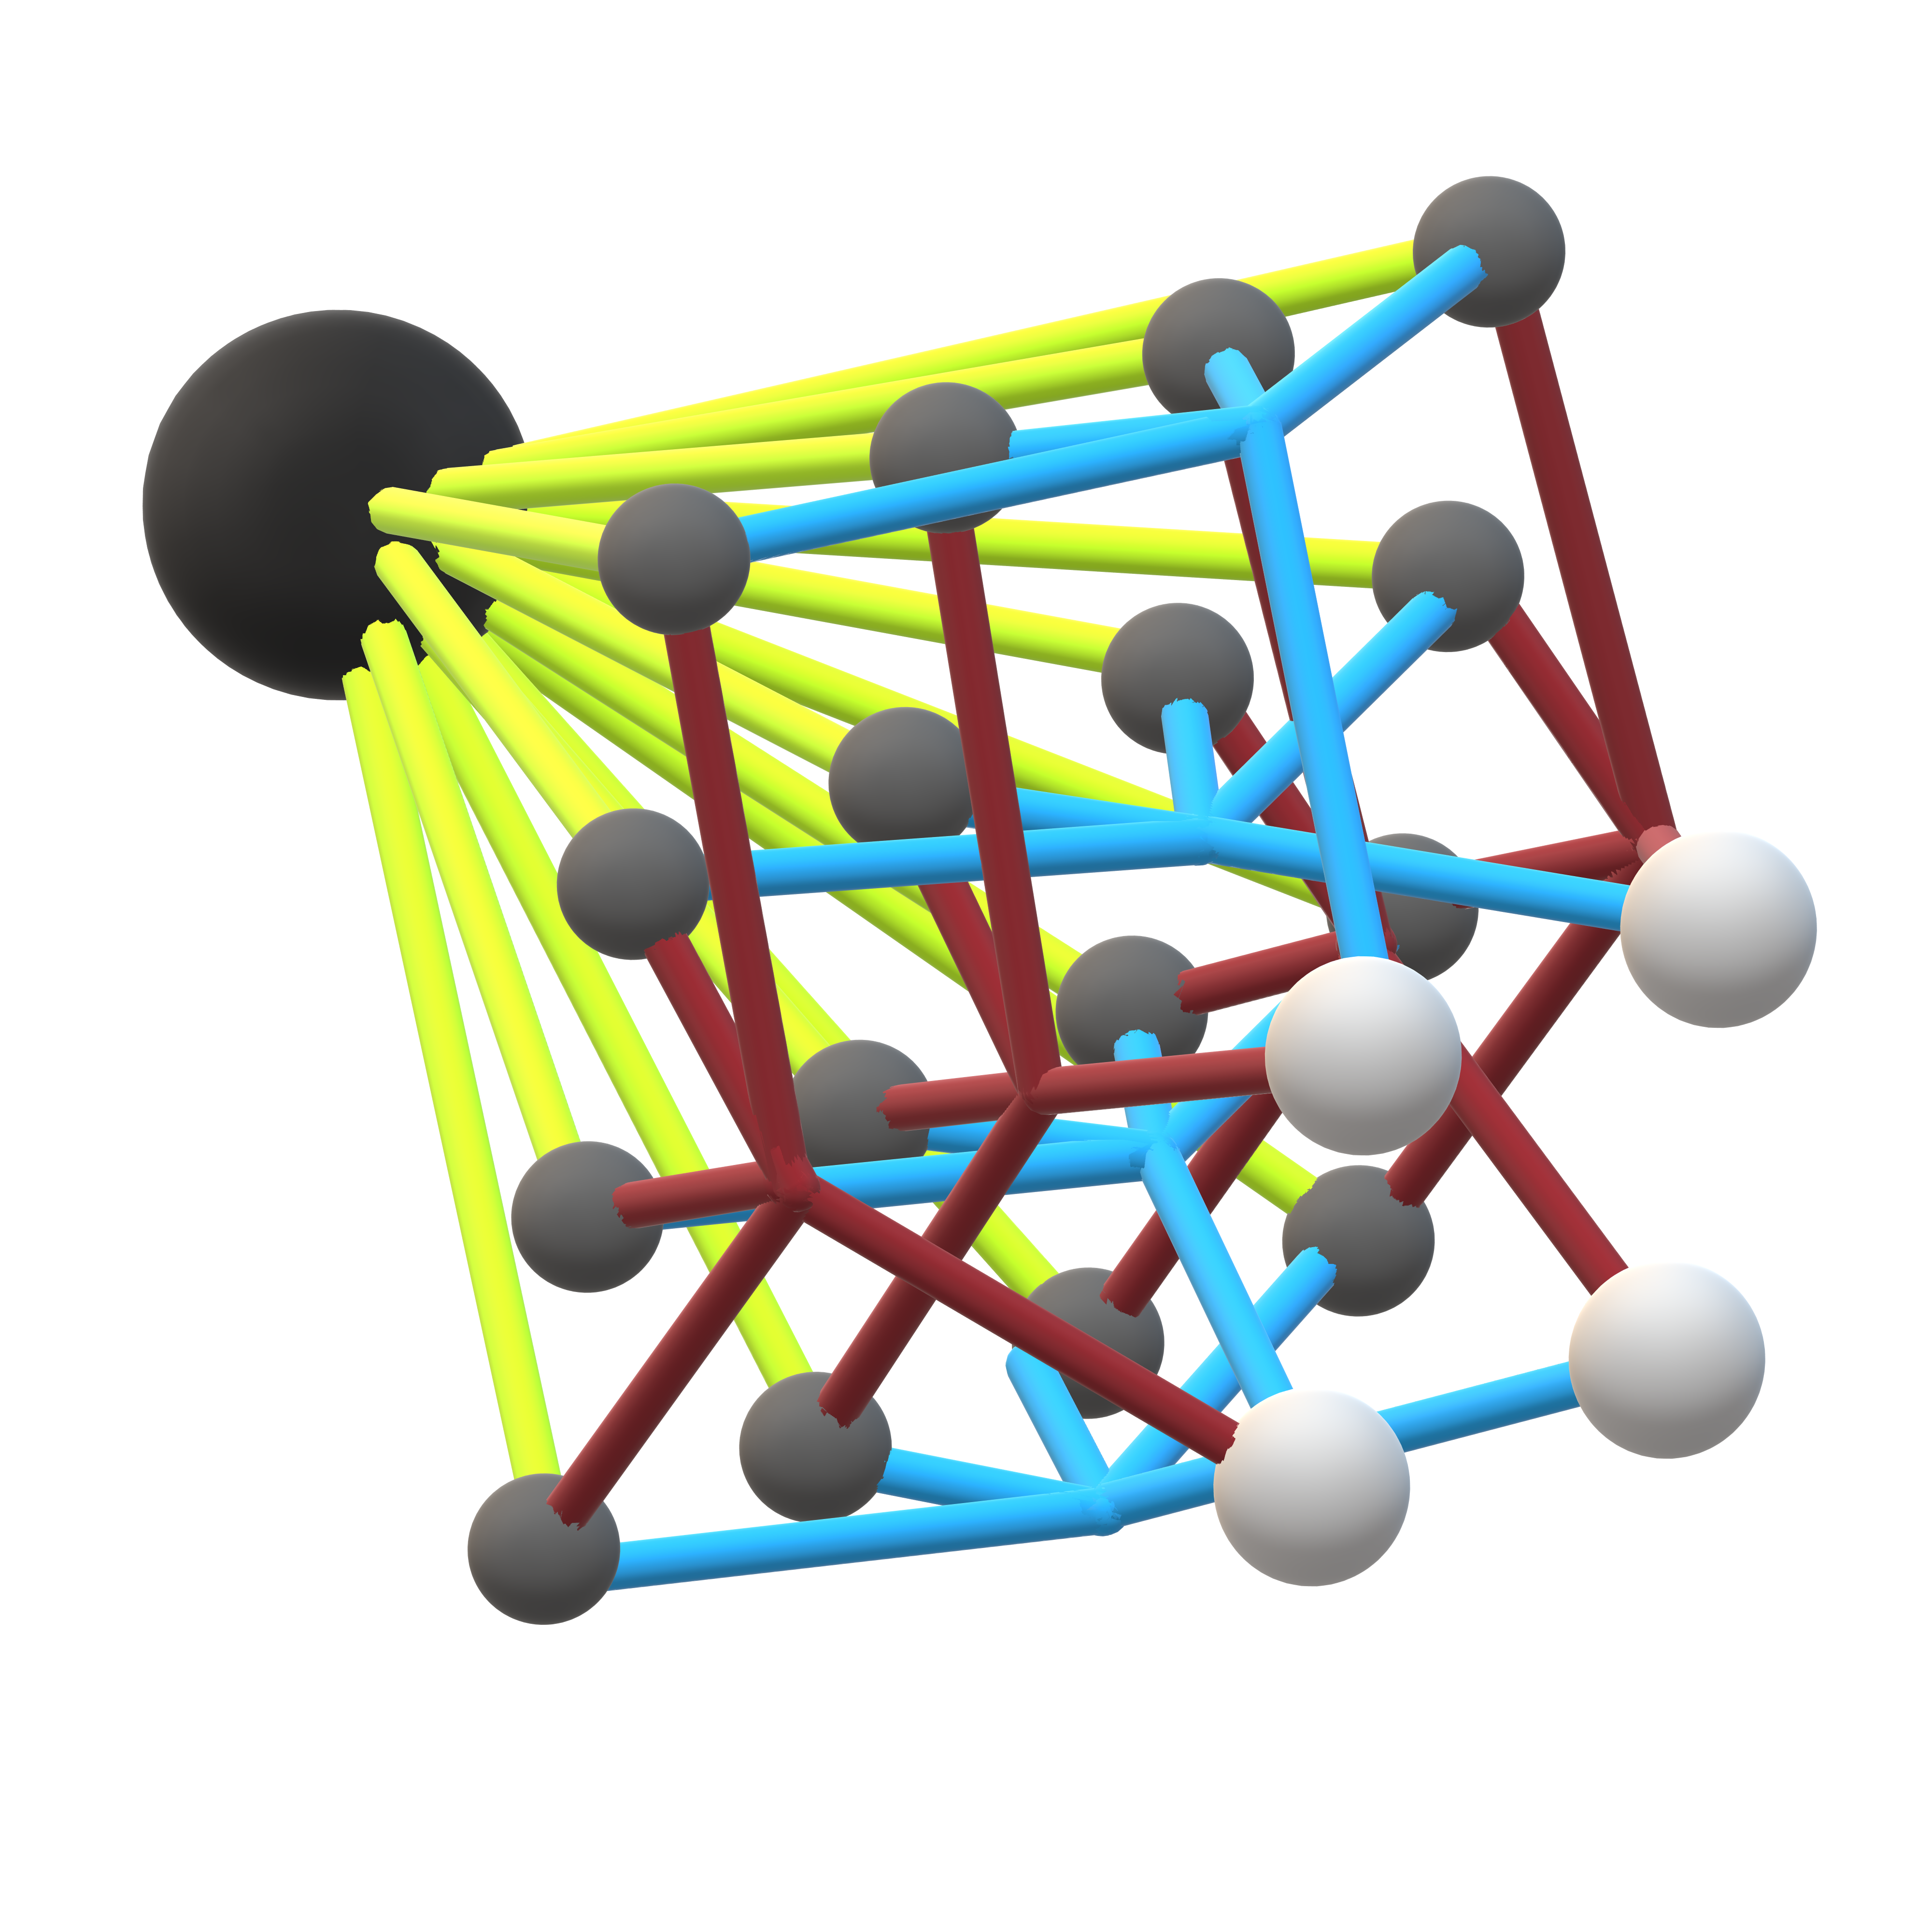
\includegraphics[width = 2in]{Friendly/LaTeX/figures/pairwiseview1.png} & 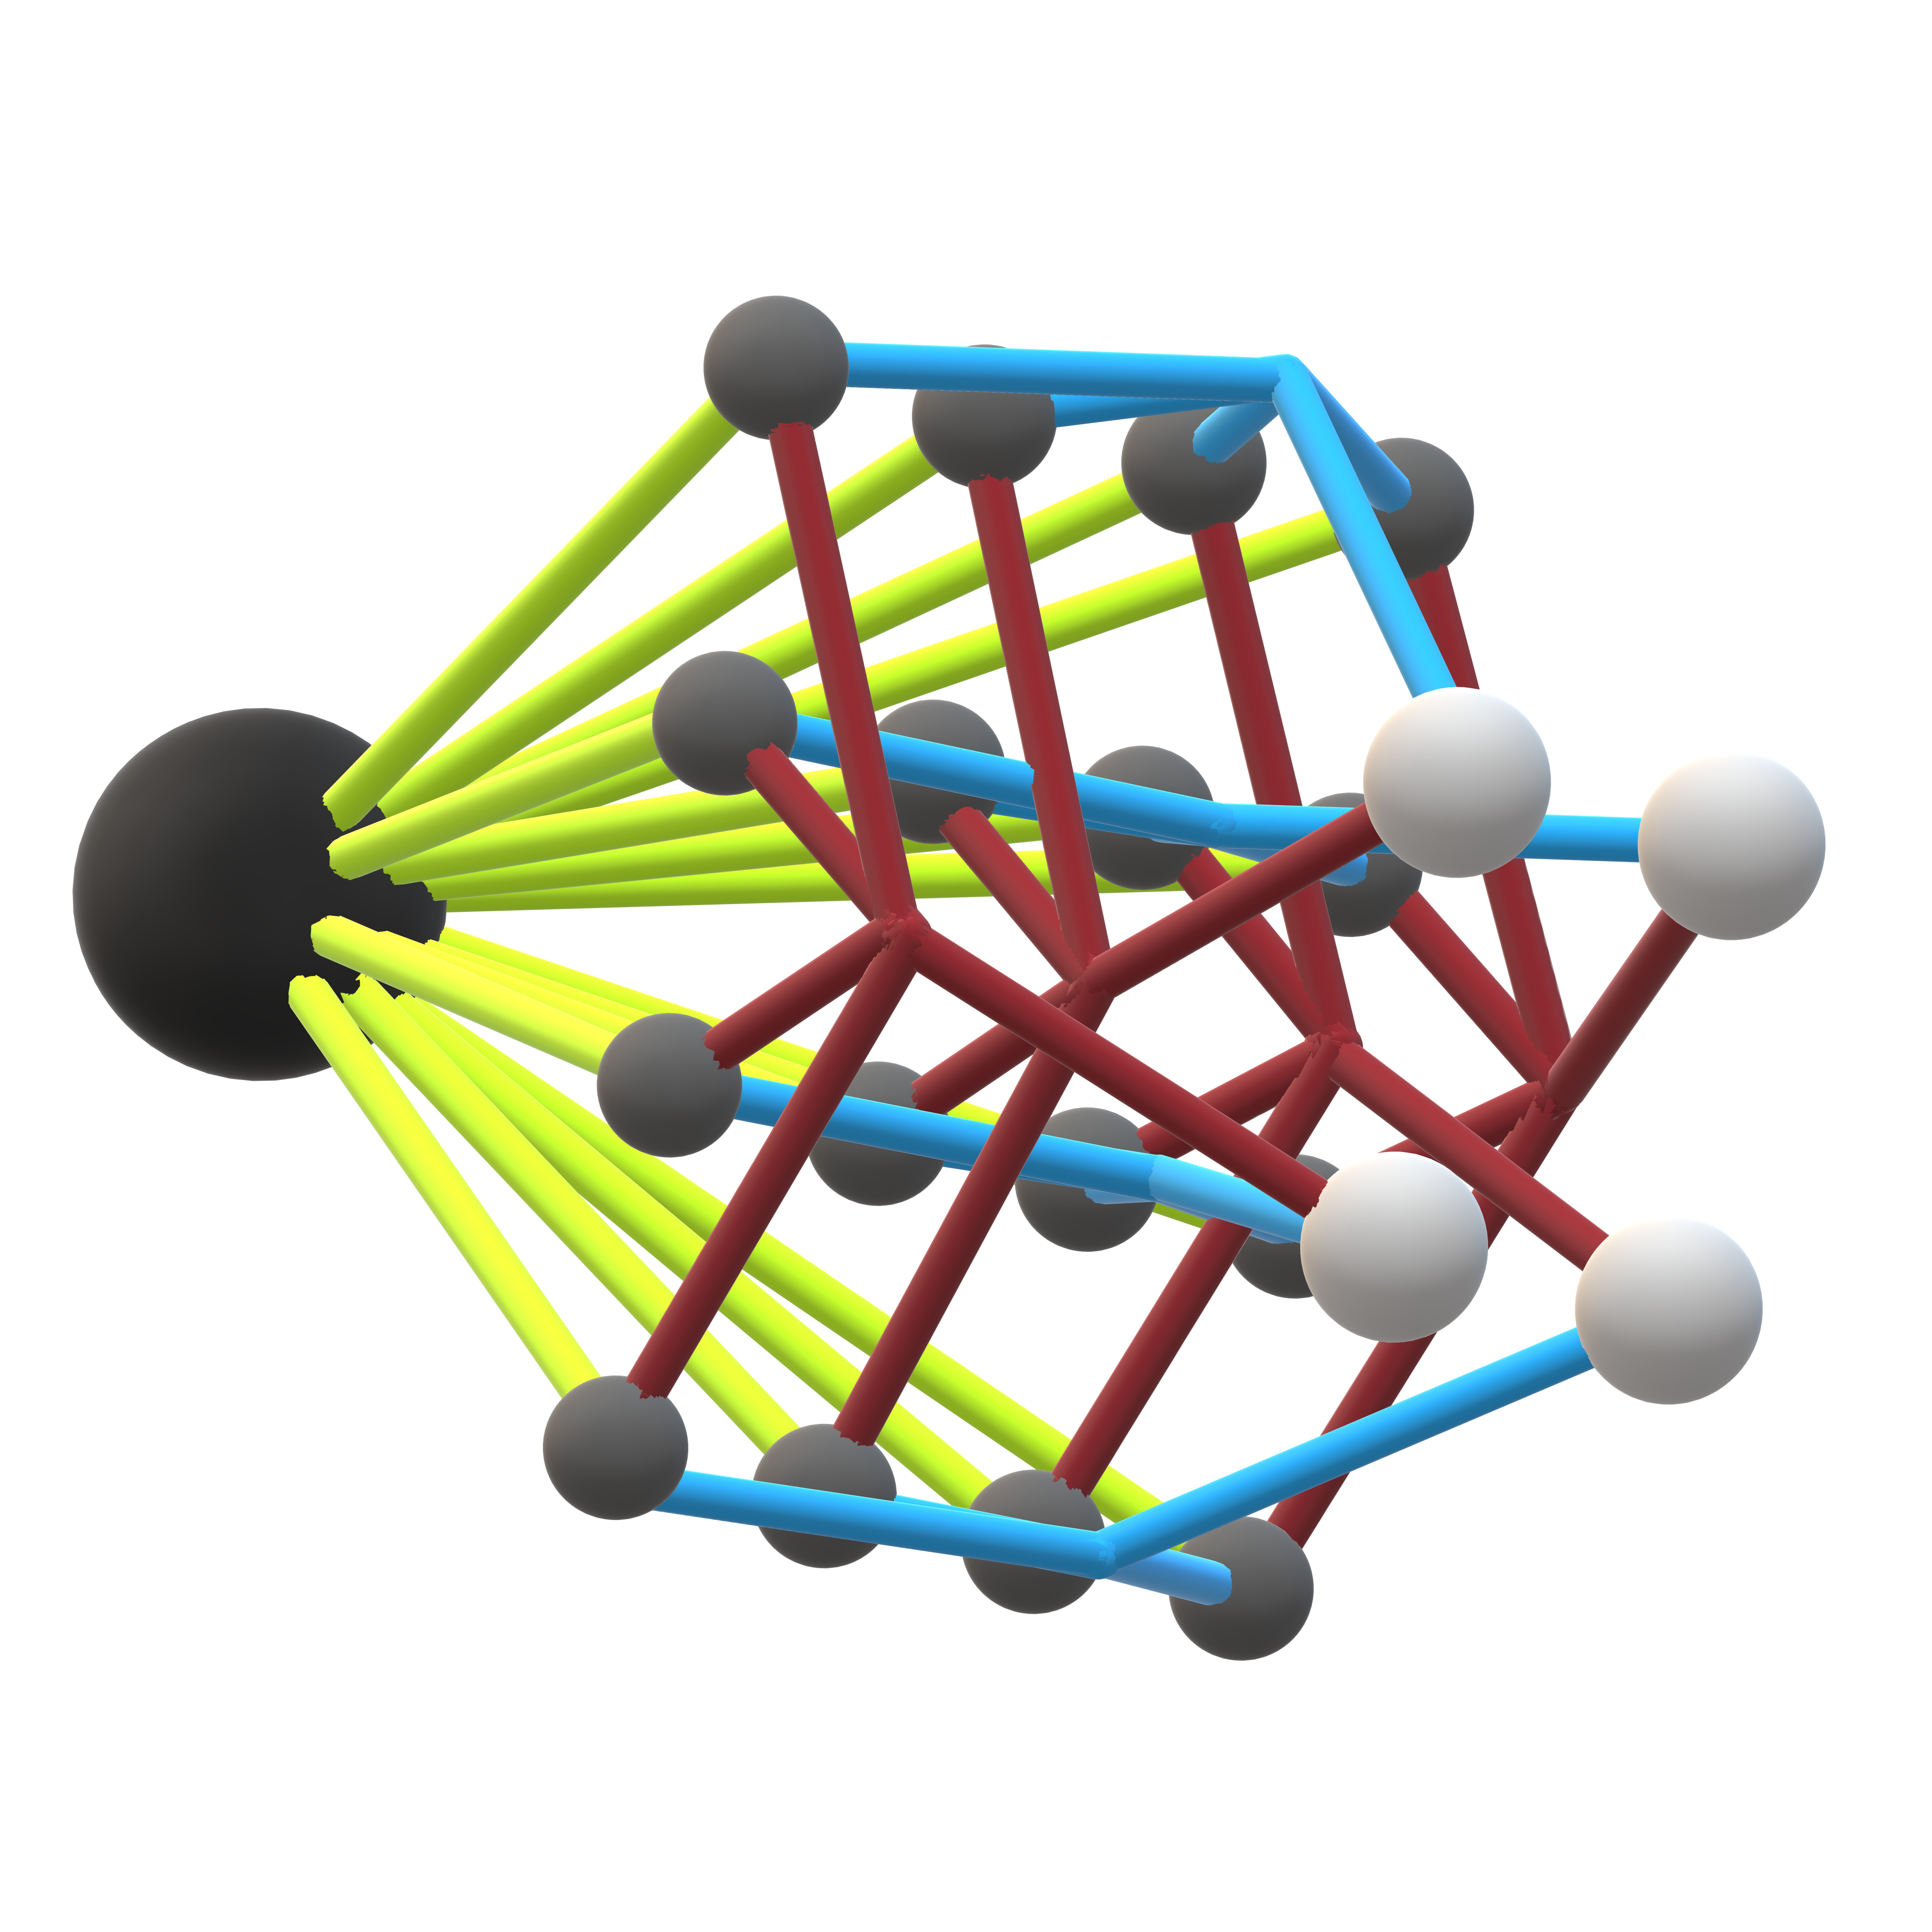
\includegraphics[width = 2in]{Friendly/LaTeX/figures/pairwiseview2.png} & 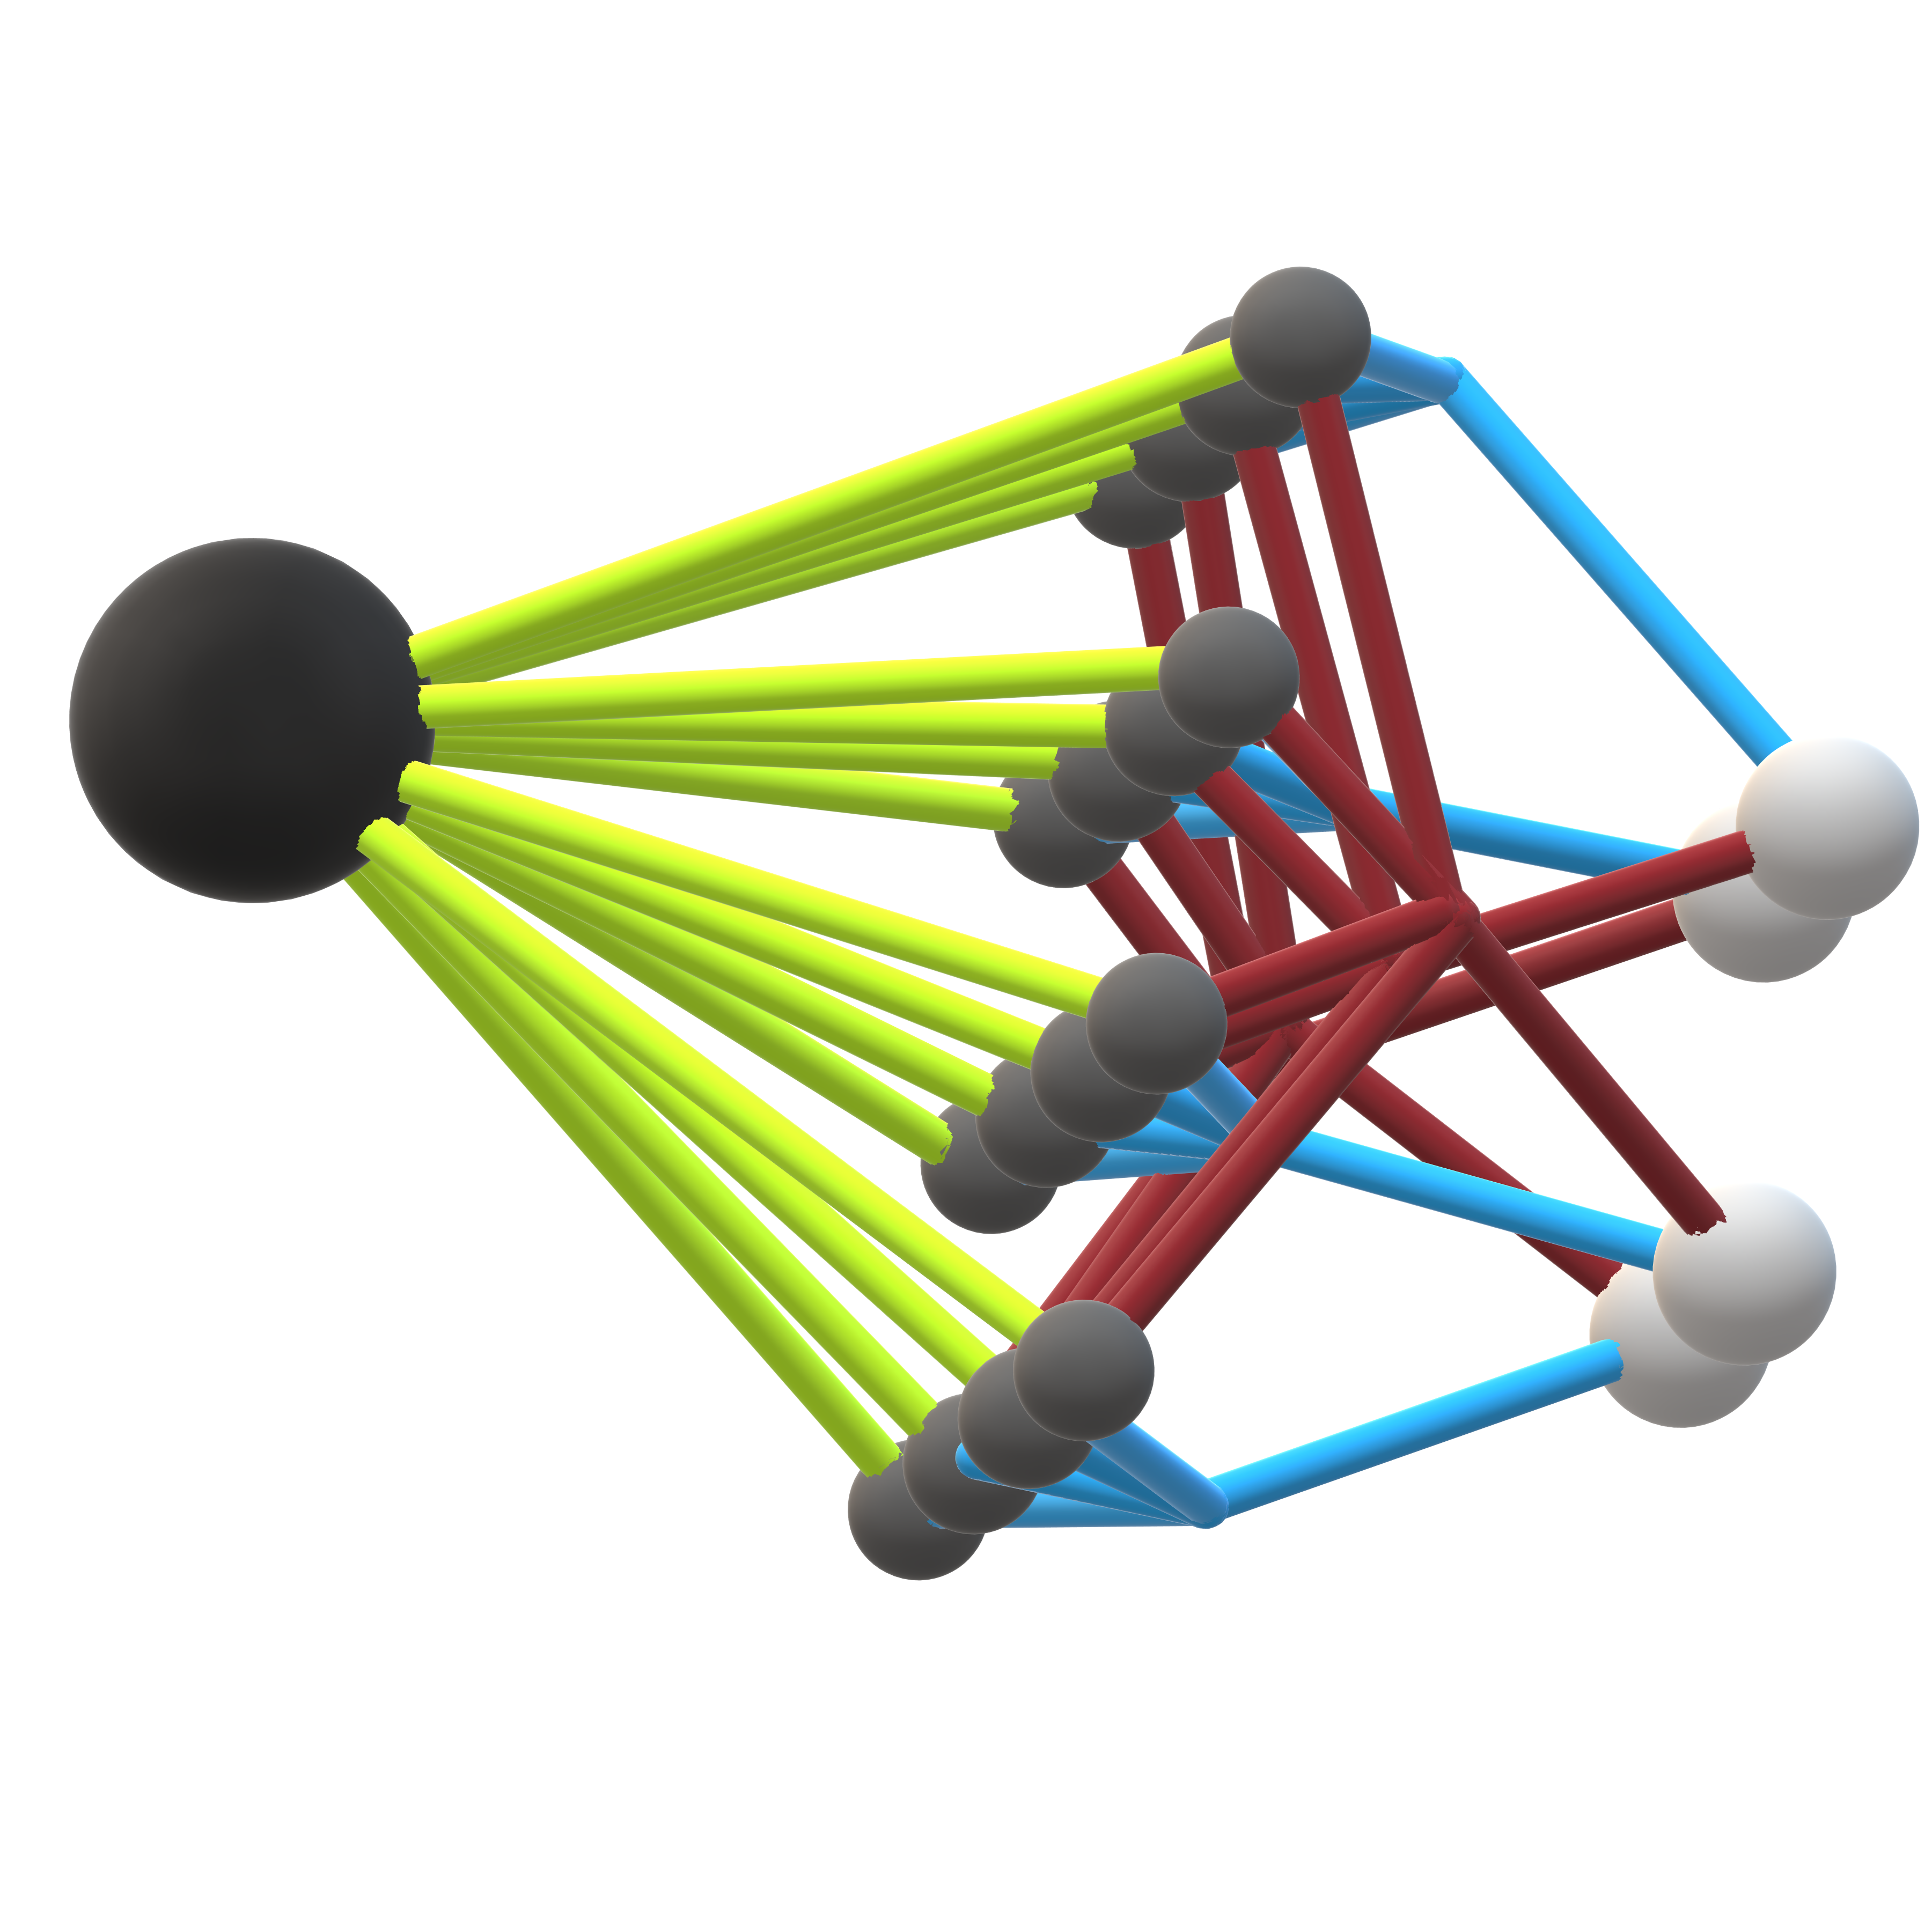
\includegraphics[width = 2in]{Friendly/LaTeX/figures/pairwiseview3.png}
        \end{tabular}
    \end{center}
    \caption{Visual of Pairwise Difference. From light to dark, the spheres represent the input, the
             subtaction + sigmoid, and the output of pairwise difference (sans the activation
             function). Burgundy lines indicate that the value it links from is being subtracted
             from the teal line's equivalent. Generated using Paint 3D~\cite{msftprogram}.}
    \label{pairwisedepiction}
\end{figure}

The difference matrix alone does not actually solve the problem described in
\cite{goodfellow2015explaining}; this is because, if all these subtractions are used in a neuron by
multiplying each subtraction by one of the neuron's weights, noise added to a patch causes noise in
the subtractions, which leaves us at the same issue (or possibly even worse given the squared number
of elements, although we have not done the math to prove this claim). Further, we just want to know
how the subpixels compare, not how they subtract. As a result, before the dot product of the neuron,
we put each subtraction through a sigmoid activation function. At the first layer, if the input
contains integer values (as is the common representation of subpixels), we won't see much change in
the sigmoid in the face of noise as the range of values is typically 0 to 255, whereas the sigmoid
activation function plateaus not far (relatively speaking) from the origin. This is the benefit of
pairwise comparisons: small changes in a subpixel values do not have the same effect on the
comparison (just between two subpixels) as it does on a dot product. To wrap up, the output neuron
does not require any specific activation function, as most of the flatness comes from the preceding
sigmoid functions. We call this neuron \textit{Pairwise Difference}.

However, there is still a rather large elephant in the room: computational complexity is essentially
squared, as we are building a pairwise matrix from a single vector. This is not a trivial problem to
address; for example, one might just use the non-zero values in the upper triangle of $D$ because
$D$ is antisymmetric, so the information gain of keeping the lower triangle is (hopefully) very minimal, at
least for $D$. However, this method suffers from not being able to treat the non-commutativity of
subtraction differently, as there is no weight for the second permutation of the operands of
subtraction. Further, effectively halving the number of inputs to the dot product only reduces the
dot product complexity by a constant factor, so, theoretically, larger and larger kernels, from a
practical standpoint, still might be out-of-reach. An alternative to the difference matrix might be
that, as in the ``mini-networks'' of Inceptionv3\cite{szegedy2015rethinking}, we do tiny dot
products, and then take dot products of those tiny dot products, etc. Each tiny dot product would
need to go through an activation (a pseudo-mimic of the difference matrix with just a few elements
participating in the dot product) as, otherwise, the result of the ``mini-network'' would be very
similar to a normal dot product from the perspective of \cite{goodfellow2015explaining}. A third
method would be to use this type of layer on just the image as most of the noise filtering will
likely occur within that layer.

In addition to these computational issues, when programming such layers, it is very easy for memory
complexity to grow as quickly as computational complexity. This is due to the fact that, in
frameworks such as Chainer\cite{tokui2019chainer} and PyTorch\cite{NEURIPS2019_9015}, at the very
least, it is easy to inadvertently suffer from holding the full difference matrix in memory. We can
get around this by performing the subtraction, sigmoid, and weight multiplication operations
one-at-a-time for each pair formed by a reference subpixel $p_i$ with static index $i$ and every
other subpixel $p_j$ in the kernel; if this happens for each static subpixel, we end up with a dot
product for every reference pixel, which requires a single value of appropriate size in memory.
Parallelization can still occur by doing this for each $i$ simultaneously. Note that this does not
differ from the memory requirements of holding each subpixel in memory, which is a tractable usage
of memory. However, at the time of writing, this implementation had not been finished.

From a gradient standpoint, Pairwise Difference is a little complicated. Following the intuition
of \cite{IMM2012-03274}[eqns. 136] where every path a gradient can take to a variable has a gradient
that must by multiplied by the gradient from the start of the path to the variable (this is used in the multivariable
chain rule, whose necessity was made clear to us by \cite{li}[``Gradients add up at forks'']), there are two
types of paths for our specific problem where this may be the case:
\begin{enumerate}
    \item the paths attributable to each image in the batch, and
    \item the paths inside those paths that are associated with each spot to which the neuron was
          applied
\end{enumerate}
Note that these are really just the same paths (all these paths fit case 2), but they are separated
here to show that there is a hierarchy of paths, which may ease the understanding of the following
derivation of Pariwise Distance's derivative.

For one patch $p$ of one sample in the batch (that has been processed by layer $i$'s neuron, $n_i$,
contained in a Pairwise Difference layer), the output of $n_i(p)$ is a dot product between the
sigmoid-filtered subtractions between each element $r$ and element $s$ in the patch and $n_i$'s
weights, $w_{rs}$. We will call ``$\text{sig}$'' the sigmoid activation function and
``$\text{sub}$'' subtraction formulated as $\text{operand}_1 - \text{operand}_2$. The derivative
with respect to $w_{rs}$ is
\[
    \frac{\partial n_i}{\partial w_{rs}}
    = \frac{\partial}{\partial w_{rs}}  \sum_{a \in p} \sum_{b \in p} w_{ab} \cdot \text{sig}(\text{sub}(a, b))
    = \frac{\partial}{\partial w_{rs}}  w_{rs} \cdot \text{sig}(\text{sub}(a, b))
    = \text{sig}(\text{sub}(a, b))
\]
Each of the volumes (one for each sample in the batch) uses $w_{rs}$ (abstracting away $p$ so that
it represents just the patch that would be taken out at $p$'s location). According to the multivariable
chain rule, for a loss function $L$, $\frac{\partial L}{\partial w_{rs}}$ is the summation of the
partial derivatives calculated by multiplying $\frac{\partial L}{\partial n_i}$ by
$\frac{\partial n_i}{\partial w_{rs}}$.

To keep backpropagation\cite{rumelhart} going to the previous layer, we also need to know
$\frac{\partial n_i}{\partial r}$ (where, again, $r$ is in $p$). In a fashion similar to $w_i$,
$r$ participates indirectly in multiple dot products against many different weights. Not only is $r$
used in $\text{sig}(\text{sub}(r, r'))$ where $r'$ is any element in $p$, but it is used in the other direction,
$\text{sig}(\text{sub}(r', r))$. For the former, the derivative for each of these is
\[
    \frac{\partial \text{sig}}{\partial \text{sub}(r, r')} \frac{\partial \text{sub}(r, r')}{\partial r}
    = \frac{\partial \text{sig}}{\partial \text{sub}(r, r')} (1)
    = \frac{\partial \text{sig}}{\partial \text{sub}(r, r')}
\]
and for the latter, it is
\[
    \frac{\partial \text{sig}}{\partial \text{sub}(r', r)} \frac{\partial \text{sub}(r', r)}{\partial r}
    = \frac{\partial \text{sig}}{\partial \text{sub}(r', r)} (-1)
    = - \frac{\partial \text{sig}}{\partial \text{sub}(r', r)}
\]
Again, since the multivariable chain rule allows us to add all pairs of these derivatives together,
for all patches $P_r$ that contain $r$, we end up with the derivative being
\begin{multline}
    \sum_{p \in P_r} \sum_{n \in neurons} \frac{\partial n}{\partial r}
    = \sum_{p \in P_r} \sum_{n \in neurons} \sum_{r' \in p} \left[ \frac{\partial n(p)}{\partial \text{sub}(r, r')} \frac{\partial \text{sub}(r, r')}{\partial r} + \frac{\partial n(p)}{\partial \text{sub}(r', r)} \frac{\partial \text{sub}(r', r)}{\partial r} \right]\\[10pt]
    = \sum_{p \in P_r} \sum_{n \in neurons} \sum_{r' \in p} \left[ \frac{\partial n(p)}{\partial \text{sub}(r, r')} (1) + \frac{\partial n(p)}{\partial \text{sub}(r', r)} (-1) \right]\\[10pt]
    = \sum_{p \in P_r} \sum_{n \in neurons} \sum_{r' \in p} \left[ \frac{\partial n(p)}{\partial \text{sub}(r, r')} - \frac{\partial n(p)}{\partial \text{sub}(r', r)} \right]
\end{multline}
The derivatives that remain in this equation are easy to derive based on the description of Pairwise
Difference (a simple multivariable chain rule application), so we do not find it necessary to do so
here.









\subsection{Angular Neurons}
\label{cosineneurons}
Again, addressing the issue from \cite{goodfellow2015explaining} with the dot product, another
structural approach was taken. To reduce the impact of the number of elements in the input vector(s),
the cosine between the input vector and the weights was considered. There is more than one way to
view why this may address this issue. A goal of this layer is subtle: we want to make sure that
extreme dimensionality does not increase the chances of the dot product going through major change.
In the case of cosine, we can see why it may address this issue: generally (more on that later), as
the number of elements increases, the number of elements that need to change in order to change the
angle the same amount also increases. Therefore, if a very small angular neuron with, say, two
inputs, does not change easily, the idea is that one with many inputs would not either.

Using the identity $\cos(\mathbf{a}, \mathbf{w}) \left\| \mathbf{w} \right\| \left\| \mathbf{a}
\right\| = w \cdot a$, one can see that $\cos(\mathbf{a}, \mathbf{w}) = \frac{w \cdot a}{\left\|
\mathbf{w} \right\| \left\| \mathbf{a} \right\|}$. Following standard neuron implementations, we add
a linear bias term to the resulting cosine as well. To see why a decreasing derivative is the case,
consider the derivative of the cosine (we omit the bias because it disappears when differentiating
due to it having no analytical relationship with $\mathbf{w}$ and $\mathbf{a}$)
\begin{flalign}
    \frac{\partial}{\partial a} \cos(\mathbf{a}, \mathbf{w}) \notag
    &= \frac{\partial}{\partial a} \frac{\mathbf{w} \cdot \mathbf{a}}{\left\| \mathbf{w} \right\| \left\| \mathbf{a} \right\|}\\[10pt] \notag
    &= \frac{
        \left\| \mathbf{w} \right\| \left\| \mathbf{a} \right\| \frac{\partial}{\partial \mathbf{a}} w \cdot a     -    \mathbf{w} \cdot \mathbf{a} \frac{\partial}{\partial \mathbf{a}} \left( \left\| \mathbf{w} \right\| \left\| \mathbf{a} \right\| \right) 
    }{
        \left(   \left\| \mathbf{w} \right\| \left\| \mathbf{a} \right\|   \right)^2
    } & \text{quotient rule} \notag \\[10pt]
    &= \frac{
        \left\| \mathbf{w} \right\|   \left\| \mathbf{a} \right\|   \mathbf{w}      +      \mathbf{w} \cdot \mathbf{a}   \left\| \mathbf{w} \right\|   \mathbf{a}
    }{
        \left\| \mathbf{w} \right\|^2 \left\| \mathbf{a} \right\|^3
    } & \text{\protect\parbox{2.5in}{derivative of $\mathbf{w} \cdot \mathbf{a}$ and $\left\| \mathbf{a} \right\|^2$ are $\mathbf{w}$~\cite{IMM2012-03274}[eqn. 69] and $2 \mathbf{a}$~\cite{IMM2012-03274}[eqn. 131]}} \notag \\[10pt]
    &= \frac{
                w
    }{
        \left\| \mathbf{w} \right\| \left\| \mathbf{a} \right\|
    }   +   \frac{
                    (\mathbf{w} \cdot \mathbf{a}) \mathbf{a}
            }{
                    \left\| \mathbf{a} \right\|^3   \left\| \mathbf{w} \right\|
            }
    \label{angularderivative}
\end{flalign}
Because (\ref{angularderivative}) contains the cosine function $\frac{ (\mathbf{w} \cdot
\mathbf{a}) } { \left\| \mathbf{a} \right\|   \left\| \mathbf{w} \right\| }$ hidden within it, we
can cap its contribution to increasing the gradient. In fact, it can never multiplicatively increase
the operand that contains it as values of cosine are between $-1$ and $1$. If we set it to $1$ ($-1$
would only change the sign, which does not matter when it comes to the magnitude of the gradient)
for that part of the equation as a worst-case scenario (where ``worst-case'' refers to the least
favorable conditions for the defense), we are left with
\begin{equation}
    \frac{
            \mathbf{w}
    }{
        \left\| \mathbf{w} \right\| \left\| \mathbf{a} \right\|
    }   +   \frac{
                    \mathbf{a}
            }{
                    \left\| \mathbf{a} \right\|^2
            }
    = \frac{
              \mathbf{w}
      }{
          \left\| \mathbf{w} \right\| \left\| \mathbf{a} \right\|
      }   +   \frac{
                      \mathbf{a}
              }{
                      \mathbf{a}^T \mathbf{a}
              }
    \label{upperbounded}
\end{equation}
Adding an element with value $q$ to $\mathbf{a}$ (which is of length $l$) results in the second term
of the derivative's addition turning from $\frac{  (\mathbf{a} \cdot 2)  }{  \left[ \sum_{i = 0}^{l}
a^2_{i} \right]  }$ to $\frac{  (\mathbf{a} \cdot 2)  }{  \left[ \sum_{i = 0}^{l} a^2_{i} \right] +
q^2  }$. Notice that the derivative with respect to $a_i$ scales with $q^2$, so it is not an ideal
linear scaling that spreads the gradient across the vector proportionally. However, this may pass
the test of the dot product's gradient contributions described in the beginning of this section, the
only issue possibly being that the quadratic scaling imposed by $q$ may cause an inversion of the problem,
where large vectors become less affected by perturbations than short ones, at least for added $q$s
that are greater than or equal to one (the ``equal to one'' case would give us the aforementioned perfect
scaling).

In regard to the same scenario with respect to the first term, we see that that term's contribution
scales sub-linearly when adding that same $q$ to $\mathbf{a}$, as the term of the denominator is the
norm of $\mathbf{a}$, not its squared norm. This \textit{reduces} the dot product issue, but does
not completely mitigate it. However (though we have not analytically shown it), when in combination
with the second term's scaling, it may be that they cancel out somewhat to give us a more linear
scaling overall. The conjectures about this second term of the addition depend on $\mathbf{w}$'s
requisite increase in the number of elements not throwing a wrench in the works; however,
$\textbf{w}$ is static at test time, so this may not matter.


It is important to note that, in the end result of (\ref{upperbounded}), the term on the right is
divided by the squared norm of $\mathbf{a}$, our input. If the elements of $\mathbf{a}$ become too
small, you start to see that fraction grow in magnitude (because $a^T a \to 0$, while each
individual element of $a$ that it is divided by decreases linearly). In the case of
MNIST\cite{lecun}, this becomes a serious issue if the images are fed directly into the network;
this is due to the fact that the inverted version of MNIST (as used in \cite{szegedy2014intriguing})
has many locations where the input $\mathbf{a}_0$ into layer $0$ of an image (a) completely, or (b)
almost completely consists of zero elements. For case (a), the derivative is even undefined. There
is a simple solution to this, however. If we put a constant value $c$ into the denominator of the
cosine, the derivative becomes
\begin{flalign*}
    &\frac{\partial}{\partial a} \frac{\mathbf{w} \cdot \mathbf{a}}{\left\| \mathbf{w} \right\| \left\| \mathbf{a} \right\|}
    = \frac{
        \left\| \mathbf{w} \right\| \left\| \mathbf{a} \right\| \frac{\partial }{\partial \mathbf{a}} \mathbf{w} \cdot \mathbf{a}     -    \mathbf{w} \cdot \mathbf{a} \frac{\partial }{\partial \mathbf{a}} \left( \left\| \mathbf{w} \right\| \left\| \mathbf{a} \right\| + c\right) 
    }{
        \left(   \left\| \mathbf{w} \right\| \left\| \mathbf{a} \right\|   +   c \right)^2
    } & \text{according to the quotient rule}\\[10pt]
    &= \frac{
        \left\| \mathbf{w} \right\|   \left\| \mathbf{a} \right\|   \mathbf{w}      -       \mathbf{w} \cdot \mathbf{a}   \left\| \mathbf{w} \right\|   \mathbf{a} \cdot 2
    }{
        \left(   \left\| \mathbf{w} \right\| \left\| \mathbf{a} \right\|   +   c    \right)^2   \left\| a \right\|
    } & \text{\cite[eqn. 69]{IMM2012-03274} and \cite[eqn. 131]{IMM2012-03274} again}\\[10pt]
    &= \frac{
        \left\| \mathbf{w} \right\|   \left\| \mathbf{a} \right\|   \mathbf{w}      -       \mathbf{w} \cdot \mathbf{a}   \left\| \mathbf{w} \right\|   \mathbf{a} \cdot 2
    }{
        \left(   \left\| \mathbf{w} \right\| \left\| \mathbf{a} \right\|^2   +   2c \left\| \mathbf{w} \right\| \left\| \mathbf{a} \right\|   +   c^2     \right)   \left\| a \right\|
    } \\[10pt]
    &= \frac{
        \left\| \mathbf{w} \right\|   \left\| \mathbf{a} \right\|   \mathbf{w}      -       \mathbf{w} \cdot \mathbf{a}   \left\| \mathbf{w} \right\|   \mathbf{a} \cdot 2
    }{
        \left(   \left\| \mathbf{w} \right\|^2 \left\| \mathbf{a} \right\|^3   +   2c \left\| \mathbf{w} \right\| \left\| \mathbf{a} \right\|^2   +   c^2     \right)
    }
\end{flalign*}
Notice that, as the norm of $\mathbf{a}$ increases, this modification starts to look more like what
you would get from cosine, and the derivative does the same with respect to cosine's derivative (for
the latter case, $\left\| \mathbf{w} \right\|^2 \left\| \mathbf{a} \right\|^3$ drastically outpaces
both the $2c \left\| \mathbf{w} \right\| \left\| \mathbf{a} \right\|^2$ term, and $c^2$ stays
constant). Therefore, we get the reduced derivative behavior of cosine for large norms. As
the norm gets smaller, the first and second aforementioned terms go to $0$, leaving us with the
third constant term. When this occurs, the cosine transforms into a scaled dot product (with scaling
factor $\frac{1}{c}$), and, as a result, the derivative (by \cite{IMM2012-03274}[eqn. 69]) becomes
$\frac{1}{c^2} \mathbf{w}$, thus avoiding the trend of the derivative going to infinity. A downside
is that $\mathbf{a}$s that cause this dot product-like behavior do not get the same protections as
what is afforded by cosine. Further, at the time of writing, it is not clear to the author if and
when a certain value of $c$ is needed to prevent adversarial examples from exploiting even a little
boost to the derivative by a shrinking norm.



\section{Evaluation}
\subsection{Evaluation Procedures}

One of the go-to~\cite{szegedy2014intriguing, kannan2018adversarial} datasets when it comes to
testing defenses is MNIST~\cite{lecun}. Modern papers~\cite{kannan2018adversarial,
tramèr2020ensemble} use ImageNet~\cite{ILSVRC15} as a training/assessment database. However we did
not get to considering ImageNet due to deadlines. So, we kept our evaluation to MNIST\footnote{MNIST
was suggested by Ali Varamesh as well; he was inspired by \cite{szegedy2014intriguing} and
\cite{goodfellow2015explaining}}. This dataset involves 70,000 images, 60,000 of which are meant for
training, and 10,000 for testing. We chose 4,200 of the 60k as validation images (used for early
stopping), and 55,800 used for the optimization procedure. The validation dataset was not subject to
an adversary. Moving on, each image is 28 pixels wide and tall, with a single channel that
represents grayscale data. The maximum value of a pixel is 255 (with the minimum at 0); however,
unlike what is common in imagery, 255 represents black, and decreasing values cause increasing
whiteness. This is an important point: \cite{szegedy2014intriguing}, for example, understandably,
has 0 and 255 be the black and white, respectively. In order to be consistent with testing, we
followed their assumption and did this same. Following \cite{szegedy2014intriguing}, in which they
claim to have trained their networks for perfect \textit{training set} classification, we
unsuccessfully tried to do the same, but got close\footnote{We had seen a reference that did not
achieve this either, implying that we are not alone and this might be normal, but have lost track of
the reference}.

We chose the ``FC-100-100-10'' network from \cite{szegedy2014intriguing} as our test network.
However, it was necessary in some cases to modify the network as Pairwise Difference and Angular are
not standard neurons. Further, in the latter case, we didn't use an activation at all; this is due
to cosine having curvature and putting out values between -1 and 1 (note that these values are
actually scaled depending on the value of its denominator constant). For Pairwise Difference, we
used sigmoid as the final output of the layer. Because FC-100-100-10 is fully-connected, this meant
that both Pairwise Difference and Angular took as input the output of the last layer or the image
itself. Finally, the Pairwise Difference (which was only used for the first layer due to its
pixel-oriented nature) and Angular-based networks used Batch Renormalization~\cite{ioffe2017batch},
and we trained a normal FC-100-100-10 network with Batch Renormalization for the purposes of an
ablation study (as we had found in the past that Batch Normalization~\cite{ioffe2015batch} acted as
a defense itself). In fact, the results for the network outside of ablation are interesting from an
adversarial standpoint, so we include them for that reason as well.

Our complete implementation, found at \cite{mycode}[Friendly], used Chainer~\cite{tokui2019chainer,
language, 2020NumPy-Array, cupy_learningsys2017}. The training procedures outside of what has been
described were very straightforward. We used momentum-based Stochastic Gradient Descent, and
learning rates varied to fit the model more appropriately; momentum was kept the same for all
models, as well as the batch size (20). The main reason for such a small number is that Pairwise
Difference can use up a lot of memory, and we thought it fair that all networks use the same batch
size for proper comparison. Early stopping was also employed, but none of our networks ever hit its
20 epoch limit (based on validation set performance) during the 100 epoch hard ``deadline'', so to
speak. Prediction loss was based on mean squared error, and it was formulated as
\[
    \frac{1}{s} \sum_{i=1}^{s} (\mathbf{c}_i - \mathbf{o}_i)^T (\mathbf{c}_i - \mathbf{o}_i)
\]
where $s$ is the number of samples in the batch, $\mathbf{c}$ is the correct confidence vector
(a.k.a.\ one-hot), and $\mathbf{o}$ is the outputs of the network for sample $i$. In the case of the
network whose derivative is penalized, that penalty is given a weight of 0.5, while the mean squared
error term has weight 1.0. See table \ref{settings} for the full list of hyperparameter settings
that vary between networks. Note that we tried only to follow through mostly with point 2 and
partially with point 1 in \ref{oggafsoscdtae}; time prevented us from exhausing all three points.
Specific to point 1, we do not achieve the properties ``any compelling threat model should at the
very least grant knowledge of the model architecture, training algorithm, and allow query
access''~\cite{athalye2018obfuscated}[§ 6.1] and ``[it] is not meaningful to restrict the
computational power of an adversary artificially (e.g., to fewer than several thousand attack
iterations)''~\cite{athalye2018obfuscated}[§ 6.1].
\begin{table}[th]
    \begin{center}
        \begin{tabular}{| c | c | c | c | c | c | c |}
            \hline
                                  &     S       &     RS      &   A     &     GMR     &  PD       \\
            \hline
            Batch Renormalization &     no      &     yes     &   yes   &     no      &  yes      \\
            Activation function   &   sigmoid   &   sigmoid   &   N/A   &   sigmoid   &  sigmoid  \\
            Learning rate         &    0.002    &    0.002    &         &    0.002    &  0.002    \\
            \hline
        \end{tabular}
    \end{center}
    \caption{``S'' stands for ``Standard'', ``RS'' for ``Renormalized Standard'', ``A'' for
             ``Angular'', ``GMR'' for GMR, ``GMRES'' for the addition of Elastic Sigmoid to GMR, and
             ``PD'' for ``Pairwise Difference''}
    \label{settings}
\end{table}
As is stated in \cite{athalye2018obfuscated}, it is important to conduct tests using a separate
network for generating adversarial examples due to ``gradient masking'' (as a reminder, this is an
effect where the trained network can handle attacks that use the network's gradient, while not being
able to handle other kinds of attacks; this author only knows of gradient-based attacks which use a
different network, but there may be something he is missing). As a result, they recommend black-box
attacks, where attacks are performed not using any internal values (such as the gradient) from the
network being tested. As a result, we also show black-box results where we train
another\footnote{~\cite{madry2019deep, szegedy2014intriguing} are the inspirations for ``another''}
original, non-protected network provides the adversarial examples to each of the defended networks.
The results on the MNIST test set can be found in table \ref{defensiveproficiency}. We followed
\cite{madry2019deep} and used the $[0, 255]$ equivalent (77) of the 0.3 (out of 1.0) $L_\infty$
noise that they chose. We use $L_{\infty}$ as it is used throughout the literature
(\cite{goodfellow2015explaining, madry2019deep, tramèr2020ensemble}, etc) and is the easiest to
program for. To disclose discrepancies in performance under normal circumstances, we present table
\ref{clean}.

\begin{table}
    \begin{center}
        \begin{tabular}{| c | c | c | c | c | c | c |}
            \hline
                             &      S      &    RS     &    A     &   GMR     &   GMRES   &   PD     \\
            \hline
            White-box (FGSM) &  46.16\%    &  43.30\%  &  0.53\%  &  37.67\%  &  36.98\%  &  32.20\% \\
            Black-box (FGSM) &  45.28\%    &  45.27\%  &  56.35\% &  43.24\%  &  44.70\%  &  49.87   \\
            \hline
        \end{tabular}
    \end{center}
    \caption{Performance of each network when it comes to black-box and white-box attacks.
             Table \ref{settings}'s caption has the meaning of the top-row acronyms.}
    \label{defensiveproficiency}
\end{table}

\begin{table}
    \begin{center}
        \begin{tabular}{| c | c | c | c | c | c |}
            \hline
            S        &     RS    &     A     &   GMR    &   GMRES   &   PD     \\
            \hline
            95.86\%  &  97.73\%  &  85.09\%  &  96.09\% &  96.72\%  &  95.91\% \\
            \hline
        \end{tabular}
    \end{center}
    \caption{Same layout as table \ref{defensiveproficiency}, but the networks were not attacked.}
    \label{clean}
\end{table}

\subsection{Outcomes}

The results turned out to be poor. It is questionable whether or not we can make any claims
whatsoever. Angular's adversarial performance was just bad (even relative to a normal network
without defenses) when up against a white-box attack, a surprising find. It did do pretty well for
the black-box equivalent, but, again, its performance in table \ref{clean} makes this network nearly
useless considering that most scenarios in real life will not be adversarial. It also turned out
that there was no point to ablation because there were no benefits of using Batch (Re)normalization.
Speculation about the results can be found in \ref{analysis}.


\subsection{Analysis}
\label{analysis}

The performance of an Angular-based network is simultaneously surprising and possibly easy to
explain. The first rationale could be that we did not pick an adequate constant to nullify the
aforementioned issue of many of zero-length vectors. None of these vectors actually ended up a zero
because each of them contained the whole image (a vector with all-zero values would contain no
number pixels), but the constant may cause issues regardless if not chosen properly. However, a more
likely scenario is that the scaling of the gradient with the addition of more elements is not as
good as hoped. As stated previously, ideally the gradient of each element in the input vector of an
Angular neuron contributes a normalized amount such that all partial derivatives in the vector add
up to, roughly speaking, the same value as when using a small patch as input. Such a neuron would
not be too dissimilar from Angular, but coming up with the formulation that we would want probably
entails integrating from the derivative that we want. We may even be able to drop normalizing the
weight vector by dividing it by $\left\| \mathbf{w} \right\|$ entirely, seeing as it is held
constant at time of attack. Though hardly fleshed-out, we would need to integrate something similar
to $\frac{\mathbf{a}}{\left\| \mathbf{a} \right\|_1}$ (this does not involve the weight vector, so
this integration is more complicated than what is shown).

As far as Pairwise Difference, the most likely explanation is that most pairs involve a comparison
between two zero-value pixels, which puts each subtraction squarely in the middle of the sigmoid
used for comparison. As a result, even FGSM using a max-norm of just 10 has a reduced 34.50\%
accuracy. It is possible that treating each comparison as a miniature neuron with two weights (or
even a bias) could be a fix for this issue because, as previously stated, this would still attempt
to address the issue of large vectors in dot products.

Renormalization appears to have been worse for the original network, which actually checks out. This
is due to the fact that \cite{ioffe2015batch} states that Batch Normalization~\cite{ioffe2015batch}
(Renormalization's predecessor) aims to keep the input to the activation function centered near, and
tight around, the origin (at least in the case of the sigmoid function) which is where the strongest
gradients lie. While this is a blessing for optimization during training, it's also a blessing for
any attacker who uses gradients in their attacks. It is possible that one conclusion that should be
drawn from this is that a Batch Renormalization-trained network in Batch Normalization mode appears
to be detrimental from a defensive standpoint.

Gradient Magnitude Reduction's lack of usefulness is concerning. The theory behind GMR, at least
intuitively, makes sense, and this may just come down to using the wrong weight in the loss term
involving the gradient w.r.t.\ the image. However, an important point to raise is that GMR does not
make any guarantees about reducing the gradient in any location other than at the point at which the
gradient is calculated. It may help to penalize even the second derivative (as it has a hand in
determining the first derivative in other locations), but the Universal Approximation
Theorem\cite{HORNIK1989359} makes it possible that even the second derivative may not be enough
seeing as there may be a valid third derivative, fourth derivative, etc. It is relevant to note that
adversarial training side steps this issue by essentially reducing the gradient at points far
(relatively speaking) from the normal datapoint, forcing (according to the evidence) all derivatives
(not just the first) to be close to zero. Elastic Sigmoid paired with GMR was ineffective as well,
for the same reasons.

Clearly, we have good reason to look further into all the defenses proposed; future work will need
to be responsible for doing so. We also need to consider Projected Gradient
Descent~\cite{madry2019deep} as an attack, as recommended by \cite{athalye2018obfuscated} because of
its effectiveness.

% At David's request^^^numbering^^^, this chapter now has a number
\chapter{Conclusion}
Representation is a very important part of neural networks (and machine learning in general). We
have put an emphasis on subitization as well as adversarial examples in order to discuss this topic,
and shown what appears to be success in representation learning via learning to count. More complex
situations need to be explored, as well as changes to and full implementation of our detection
methods to really make it work, and what we have seen with our experiments hints at this truly being
possible. We did not demonstrate a network with full subitization capabilities, but modifications to
the training and/or network may make this a reality.


As for adversarial examples, we did not have success, but we did lay out substantial justification
for the defenses that we proposed; hopefully, this analysis leads us to (a) related method(s) that
corrects for any analytical flaws in what we have proposed. Specifically, we emphasized structure
over additional loss terms, with the exception of GMR. However, even a modified form of GMR, in the
future, might benefit from structural changes, such as when any of these modifications are used in
conjunction with methods such as Elastic Sigmoid. While papers like \textit{Adversarial Logit
Pairing}~\cite{kannan2018adversarial} appear to be very close to a cure, the space of attacks seems
boundless, and this author believes that mathematical proofs are required in order to fully address
this issue. In the author's opinion, proving that iterative optimizers and special loss terms really
achieve ideal networks is difficult due to the dynamic nature of these methods and the infinite set
of points over which they are optimizing. Seeing as methods like Adversarial Logit Pairing and
adversarial training are defenses that fit within this definition, the author is somewhat skeptical
about their true effectiveness. This is because adversarial examples like what can be found in
~\cite{eykholt2018robust} focus on fooling networks relative to \text{all} human perception, and
noise bounded by $L_{\infty}$ or similar metrics clearly does not model this. Structural changes
appear easier to prove (from an adversarial example view), so they may make the most sense to pursue
further. In the end, we look into this topic because the adversarial example community inherently
focuses nearly completely on representation.

In summation, topic of representation needs substantially more resources dedicated to it. For the
author, this thesis is merely a starting point, and we plan to build upon this work. We need to
solidify the fundamentals before we can truly unleash deep learning.

%                                                                                                  %
%%%%%%%%%%%%%%%%%%%%%%%%%%%%%%%%%%%%%%%%%%%%%%%%%%%%%%%%%%%%%%%%%%%%%%%%%%%%%%%%%%%%%%%%%%%%%%%%%%%%




\addcontentsline{toc}{chapter}{Bibliography}

% This line was in here originally, but needed to be removed
% \bibliographystyle{alpha}

% Ben
%%%%%%%%%%%%%%%%%%%%%%%%%%%%%%%%%%%%%%%%%%%%%%%%%%%%%%%%%%%%%%%%%%%%%%%%%%%%%%%%%%%%%%%%%%%%%%%%%%%%
%                                                                                                  %

% Removed the appendix code and the \newpage above it from this file because I didn't need it and
% ^^^iulatex^^^ said I could.

\printbibliography

% ^^^cv^^^ says I need to put in a CV, so here it is. We have this document render it because
% the iuphd class^^^classfile^^^ sets all the correct formatting found at ^^^cv^^^
\renewcommand{\baselinestretch}{1.0}
\selectfont
\newpage
% i. https://graduate.indiana.edu/thesis-dissertation/formatting/masters.html; Master's: Formatting:
% Theses & Dissertations: The University Graduate School: Indiana University Bloomington; 2021.12.31
% visit date
%
% ii. https://owl.purdue.edu/owl/job_search_writing/resumes_and_vitas/writing_the_cv.html; Writing
% the Curriculum Vitae // Purdue Writing Lab; 2021.12.31 (visit date)
% 
% iii. https://ctan.org/pkg/geometry; CTAN: Package geometry; Hideo Umeki + David Carlisle
%
% iv. https://ctan.org/pkg/calc; CTAN: Package calc; Frank Jensen + Kresten Krab Thorup +
% LaTeX Contributors

% This file is separate from the thesis (from a citation standpoint), and is currently unpublished,
% authored by Ben Cutilli (me) in January of 2022. * refers to things that were commented out
% due to requirements found at (i), "Required and Optional Sections". @ (throughout this file)
% refers to sizes that were modified to work within these requirements. As stated is possible in
% (ii), we don't restrict the output to one page (which is the case for résumés). Finally, any other
% commands commented out were done so so that this file can be integrated with manuscript.tex.

% Changed this file for thesis by commenting out things and changing sizes.

%\documentclass{article}

% ^^^geometry^^^ package
%\usepackage[margin=0.35in]{geometry}
% Package from ^^^calc^^^
%\usepackage{calc}



%\begin{document}

\setlength{\tabcolsep}{0.1in}
\pagenumbering{gobble}

\begin{center}
    \begin{LARGE}
        Benjamin V. Cutilli
    \end{LARGE} \\
    % (ii) says that I need to include information on how to be reached
    \begin{large}
        benvcutilli@gmail.com \\
        % *
        %(215) 421-9125 \\
        % *
        %803 Nesbitt Road, Maple Glen, PA 19002
    \end{large}
\end{center} \vspace{0.5in}







% Education goes first according to (ii), and also in general I avoid listing job info until
% the end, as advised by that resource as well.
\begin{LARGE}
Education
\end{LARGE} \vspace{10pt}

\begin{center}

    % I've used tables to create columns/rows for things that aren't really tables, so I use that
    % strategy here; @
    \begin{tabular}{p{2.0in} p{4.0in}}
        Indiana University Bloomington
                                       &
                                          % Regarding *, I will have technically graduated in 2021,
                                          % and so I need to put that year here (they also implied)
                                          % that I should put the month, so I do that as well.
                                          Computer Science, Master of Science (2021.12) \newline
                                          Thesis: \textit{Exploring Representation Learning via
                                          Alternate Lenses} \newline
                                          \texttt{github.com/benvcutilli/CountingPlusFriendly}
                                         \\

        \vspace{16pt} \\

        Haverford College
                                       &
                                          Computer Science, Bachelor of Science (2013) \newline
                                          Thesis: \textit{Computer Vision and its Application in
                                          Self-Driving Cars} \newline
                                          \texttt{http://hdl.handle.net/10066/9003}
                                         \\
    \end{tabular} \\[0.5in]

\end{center}



% Same reason for this table and the next as for the first table of this document
%%%%%%%%%%%%%%%%%%%%%%%%%%%%%%%%%%%%%%%%%%%%%%%%%%%%%%%%%%%%%%%%%%%%%%%%%%%%%%%%%%%%%%%%%%%%%%%%%%%%%%%%
%                                                                                                      %




% Figured that this would be the thing that made the most sense to list next given that it is
% more important to a CV than the jobs section, following (ii).
\begin{LARGE}
Research
\end{LARGE} \vspace{10pt}

\begin{center}

    % @
    \begin{tabular}{p{2.0in} p{4.0in}}
       \textit{Addressing Supply Chain Risks
       of Microelectronic Devices
       through Computer Vision}
                                         &
                                            Chen, Wanyan, Rao, Cutilli, Sowinski, Crandall, and
                                            Templeman \newline
                                            IEEE Applied Imagery Pattern Recognition Workshop \newline
                                            2017, \texttt{https://ieeexplore.ieee.org/document/8457956}
                                          \\
    
       \vspace{16pt} \\


       \textit{Exploring Representation
       Learning via Alternate Lenses}
                                         &  
                                            Benjamin Cutilli \newline
                                            Master's Thesis at Indiana University Bloomington
                                            2021 \newline
                                            \texttt{github.com/benvcutilli/CountingPlusFriendly}
                                          \\
    \end{tabular} \\[0.5in]

\end{center}








% Based on the prioritizing mindset of (ii), this section may need to come last. Entries
% ordered in the aforementioned spirit as well
\begin{LARGE}
Work
\end{LARGE} \vspace{10pt}

\begin{center}

    % I write using this incorrect grammar (from a traditional perspective) in the responsibilities
    % text because that is what is said by (ii) to be necessary. Also, I prioritize positions that
    % have more to do with education and research over others as that was suggested by (ii) to be a
    % good idea. @
    \begin{tabular}{p{2.0in} p{4.0in}}

        Indiana University Bloomington
        School of Informatics
        and Computing
                              &
                                  Research Assistant         \newline
                                  Supervisor: David Crandall \newline
                                  % (ii) said to keep the grammar the same between similar
                                  % things, so this date span's format follows that of the entry
                                  % below
                                  January - May 2017 \newline
                                  Advised on research related to visual detection of flawed
                                  electronics; explored the possibility of using another method for
                                  the task; attended events related to research
                               \\

        \vspace{16pt} \\
    
        Indiana University
        Bloomington School
        of Informatics and
        Computing
                             &
                                  Associate Instructor \newline
                                  CSCI-B551 Elements of Artificial Intelligence \newline
                                  January - May 2017 \newline
                                  Assisted students taking course; graded assignments
                               \\
    
        \vspace{16pt} \\

        NVIDIA Corporation
                             &
                                  Internship, Solutions Architect group \newline
                                  2017 (June - August) \newline
                                  Developed software to demonstrate NVIDIA hardware; preliminary
                                  deep learning research; assisted others when needed
                                \\
    \end{tabular}



%                                                                                                      %
%%%%%%%%%%%%%%%%%%%%%%%%%%%%%%%%%%%%%%%%%%%%%%%%%%%%%%%%%%%%%%%%%%%%%%%%%%%%%%%%%%%%%%%%%%%%%%%%%%%%%%%%

\end{center}











%\end{document}
 

%                                                                                                  %
%%%%%%%%%%%%%%%%%%%%%%%%%%%%%%%%%%%%%%%%%%%%%%%%%%%%%%%%%%%%%%%%%%%%%%%%%%%%%%%%%%%%%%%%%%%%%%%%%%%%




% Adds a line for your CV without a page number

\addtocontents{toc}{%
  \protect\contentsline{chapter}{Curriculum Vitae}{}{}}
\end{document}
